\documentclass[10pt,twocolumn]{article}

\usepackage[utf8]{inputenc}
\usepackage[margin=1in]{geometry}
\usepackage{amsmath,amssymb,amsfonts,amsthm}
\usepackage{booktabs}
\usepackage{graphicx}
\usepackage[hidelinks,hypertexnames=false]{hyperref}
\usepackage{cite}
\usepackage{algorithm}
\usepackage{algpseudocode}
\usepackage{microtype}
\usepackage{times}
\usepackage{url}
\usepackage{array}
\usepackage{ragged2e}
\usepackage{placeins}

% Float tuning to prevent runaway floats
\renewcommand{\topfraction}{0.95}
\renewcommand{\bottomfraction}{0.85}
\renewcommand{\textfraction}{0.05}
\renewcommand{\floatpagefraction}{0.75}
\renewcommand{\dbltopfraction}{0.95}
\renewcommand{\dblfloatpagefraction}{0.75}

\newtheorem{theorem}{Theorem}

\title{\textbf{ModelVM: Virtualizing Semantic State and Model Residency for Resource-Constrained Language Model Systems}}
\author{Anonymous Authors}
\date{}

\begin{document}

\maketitle

\begin{abstract}
Deploying multi-specialist language model ensembles on resource-constrained hardware exposes an acute systems conflict: while domain-specialized open-weight models achieve superior accuracy on targeted engineering, mathematical, and coding sub-tasks, their aggregate parameter footprint (often exceeding $50$\,GB) far outstrips the physical memory of local consumer workstations and edge accelerators ($\le 8.0$\,GB RAM). Existing execution paradigms either suffer Out-Of-Memory (OOM) aborts, thrash secondary storage buses under reactive demand-paging, or experience catastrophic state degradation and compounding arithmetic drift when passing unstructured conversational transcripts across model boundaries. 

We present \textbf{ModelVM}, an integrated systems runtime that virtualizes both \textit{semantic state} and \textit{model weight residency} for multi-specialist language model workflows on memory-constrained devices. ModelVM is founded on a central architectural insight: \textbf{heterogeneous models can cooperate reliably under tight memory constraints if cumulative task state is decoupled from model-specific representations and conversational prose}. ModelVM realizes this principle through three co-designed subsystems: (1)~the \textbf{Cognitive State Protocol (CSP)}, a strongly typed 9-tuple state representation with deterministic Abstract Syntax Tree (AST) validation that replaces lossy natural language transcripts with formal mathematical and code invariants; (2)~the \textbf{Predictive Cognitive Working Set} ($W(t, k)$), which adapts Denning's working-set principles to structured execution graphs, opportunistically pre-staging upcoming weights into verified headroom while shielding resident models via reuse-distance cost accounting; and (3)~the \textbf{Multi-Objective Cognitive Scheduler}, an interpretable dispatch engine that scores candidate models across empirical capability fitness, memory footprint, bus load latency, energy, eviction penalties, and downstream reuse. 

In a controlled runtime evaluation across a $52.7$\,GB catalog of ten heterogeneous specialists under an enforced $8.0$\,GB budget, ModelVM maintains high factual retention ($R_{\text{facts}} \ge 0.940$) and calculation accuracy ($R_{\text{calcs}} \ge 0.920$) across extended handoff depths ($N=12$), with observed zero OOM aborts across evaluated $4.0$\,GB stress runs. Furthermore, in a live physical silicon deployment on an NVIDIA GeForce RTX 5070 Ti executing open-weight model instances (\texttt{llama3.1:8b}, \texttt{qwen2.5-coder:7b}, and \texttt{llama3.2:1b}), ModelVM reduces cumulative prompt context by \textbf{60.8\%} and cuts physical wall-clock execution latency by \textbf{77.2\%} ($65.05$\,s down to $14.85$\,s, comprising a \textbf{56.2\% active inference acceleration} from prompt compression and elimination of uncoordinated cold-loading stalls) with zero GPU memory faults.
\end{abstract}

\section{Introduction}
\label{sec:introduction}

The open-weight language model ecosystem has entered an era of profound domain specialization. Rather than relying solely on monolithic generalist models that attempt to master every discipline simultaneously, open-source researchers have developed highly capable, domain-specialized checkpoints. Models such as \textit{Qwen2.5-Math} achieve graduate-level formal mathematical derivation; \textit{DeepSeek-Coder} delivers state-of-the-art multi-language program synthesis; \textit{Mistral-Research} excels in archival literature extraction; and domain-tuned variants provide targeted expertise in classical mechanics, biomedical diagnosis, and financial modeling. For complex multi-step technical workflows—such as analyzing an archival scientific paper, deriving its closed-form governing equations, implementing an executable numerical simulation, and physically verifying phase-space boundaries—orchestrating an ensemble of specialized models produces reasoning deliverables that dramatically surpass the capability ceiling of any individual compact generalist.

However, deploying an ensemble of specialized models on local consumer hardware exposes an acute systems failure: \textbf{domain specialists are highly capable, but their parameter weights are massive}. A minimal catalog of ten specialized 7B--14B models requires over $52.7$\,GB of physical memory across mixed quantization formats (Q4\_K\_M, Q8\_0, FP16; $64.0$\,GB on disk). In contrast, local consumer workstations, developer laptops, and edge robotic platforms are physically constrained by memory envelopes of $8.0\text{--}16.0$\,GB of RAM. Consequently, running multiple specialist models simultaneously is physically impossible; memory capacity is an uncompromising physical ceiling, not an adjustable configuration parameter.

\subsection{The Three Systemic Barriers of Multi-Model Serving}
\label{sec:intro_barriers}

When systems designers attempt to deploy multi-specialist pipelines on memory-constrained hardware using existing deployment paradigms, execution collapses against three fundamental systems barriers:

\paragraph{1. The Memory Capacity \& Crash Barrier.}
Modern operating systems and inference runtimes possess no native mechanisms to coordinate the aggregate weight allocations of multiple deep language models. When a workflow attempts to load a second specialist alongside a resident model without strict global coordination, aggregate memory allocations immediately breach physical RAM. The operating system kernel invokes the Out-Of-Memory (OOM) killer, terminating the process catastrophically. As our empirical sweeps demonstrate, naive dynamic allocation under an acute $4.0$\,GB envelope triggers unhandled fatal process aborts in $60.0\%$ of task runs (Section~\ref{sec:results_r1}).

\paragraph{2. The State Incompatibility \& Conversational Bloat Barrier.}
When execution must transition between two disparate specialist models (e.g., passing intermediate mathematical derivations from a math model to a code synthesis model), existing multi-agent frameworks pass state by concatenating the full natural language conversation history into prompt text. This naive mechanism triggers catastrophic failure modes:
\begin{itemize}
    \item \textbf{Accumulating Context Bloat:} Conversational prompt length grows with cumulative prior-stage output ($L_{\text{ctx}} = \mathcal{O}(t \cdot \bar{L}_{\text{gen}})$). When forced into bounded context windows ($W_{\text{in}} = 4,096$), FIFO sliding-window truncation continually discards early foundational constraints.
    \item \textbf{Compounding Arithmetic Drift:} Conversational text lacks structural typing. When numerical constants and mathematical formulas are repeatedly paraphrased through conversational prose across multiple heterogeneous models, floating-point precision degrades, culminating in severe arithmetic hallucinations ($R_{\text{facts}}$ collapses to $0.180$ after 12 transitions).
    \item \textbf{Latent Incommensurability:} Because independently trained models operate over disparate hidden-state dimensions, rotary embeddings, and vocabulary tokenizers, internal KV-cache or activation tensors cannot be transferred across model boundaries without prohibitive $O(K^2)$ calibration bridges.
\end{itemize}

\paragraph{3. The I/O Bus Thrashing \& Latency Barrier.}
Because all models cannot reside simultaneously in active memory, weights must be dynamically swapped across the secondary storage bus (e.g., PCIe 4.0/5.0 from NVMe SSD to host RAM and accelerator VRAM). However, applying classical retrospective memory management (such as Least Recently Used / LRU caching) produces catastrophic bus thrashing. When a cyclic workflow alternates between mathematical derivation, code simulation, and numerical validation, LRU evicts the mathematical specialist to make room for coding weights, forcing an immediate, multi-gigabyte cold reload over the PCIe bus when mathematics is invoked again. In our baseline benchmarks, uncoordinated demand paging squanders up to $42.6$\,s in idle I/O stall time, causing paging latency to overwhelm actual GPU compute duration ($t_{\text{paging}} \gg t_{\text{compute}}$).

\subsection{The Architectural Insight of ModelVM}
\label{sec:intro_insight}

In this paper, we present \textbf{ModelVM}, a clean, pragmatic systems runtime that resolves this fundamental conflict between domain specialization and physical memory capacity. ModelVM is founded on a single unifying systems principle:

\begin{quote}
\textit{Heterogeneous language models can cooperate reliably under resource-constrained hardware budgets if cumulative task state is virtualized as a strongly typed, model-independent intermediate representation, and physical model residency is orchestrated via predictive working-set lookahead rather than retrospective demand paging.}
\end{quote}

Just as classical operating systems virtualized physical memory by decoupling virtual address spaces from physical DRAM pages, ModelVM virtualizes \textbf{semantic state} and \textbf{model weight residency}. ModelVM enables an 8.0\,GB workstation to execute a 52.7\,GB catalog of heterogeneous open-weight specialists, delivering the full reasoning capability of an unconstrained multi-model cluster on commodity edge silicon.

\subsection{Summary of Contributions}
\label{sec:intro_contributions}

This paper makes four concrete, empirically validated systems contributions:

\begin{enumerate}
    \item \textbf{Semantic State Virtualization (The Cognitive State Protocol - CSP):} We design and formalize CSP, a strongly typed, AST-verified 9-tuple state representation ($\mathcal{S}_t$) that replaces unstructured conversational transcripts. CSP isolates mathematical invariants, verified calculations, domain facts, and active artifacts from transient natural language, formally constraining verified arithmetic and state updates, with empirical factual retention $R_{\text{facts}} \ge 0.940$ and calculation accuracy $R_{\text{calcs}} \ge 0.920$ across $N=12$ transitions.
    \item \textbf{Predictive Cognitive Working-Set Management ($W(t, k)$):} We translate Peter Denning's foundational working-set theory into a forward-looking cognitive memory manager. By exploiting the explicit stage graph produced by task decomposition, ModelVM forecasts upcoming specialist requirements, opportunistically pre-staging weights into verified memory headroom while shielding resident models from eviction using reuse-distance cost accounting, slashing paging stalls by $66.7\%$ ($21.60$\,s down to $7.20$\,s).
    \item \textbf{Multi-Objective Cognitive Scheduling:} We implement an explainable, transparent 6-term utility scoring engine that dispatches execution stages to candidate models by jointly balancing empirical benchmark capability, memory footprint, load latency, energy, eviction penalties, and downstream reuse, observing scheduler regret no greater than $7.8\%$ relative to an offline prescient oracle across divergent workload topologies.
    \item \textbf{Full Factorial Decomposition and Physical Silicon Validation:} We conduct an exhaustive $2^3$ orthogonal factorial ablation study isolating the main effects and synergistic two-way interactions ($B \times C$) of our architectural primitives across the full 10-model catalog. Furthermore, we validate these runtime principles on physical GPU silicon (an NVIDIA GeForce RTX 5070 Ti with 16.0\,GB GDDR7 driven by the Ollama inference daemon), demonstrating a \textbf{60.8\% prompt token reduction}, a \textbf{56.2\% active inference acceleration} ($33.83$\,s down to $14.83$\,s), observed zero OOM failures across evaluated runs, and a \textbf{77.2\% reduction in end-to-end wall-clock time} ($65.05$\,s down to $14.85$\,s) on real open-weight checkpoints.
\end{enumerate}

\subsection{Paper Organization}
\label{sec:intro_organization}

The remainder of this paper is structured as follows. 
Section~\ref{sec:problem_formulation} establishes the formal system model, capacity inequalities, and foundational design goals. 
Section~\ref{sec:runtime_architecture} details the ModelVM runtime architecture and memory pager lifecycle. 
Section~\ref{sec:semantic_state} presents the formal specification, structural typing, and correctness proofs of the Cognitive State Protocol. 
Section~\ref{sec:predictive_residency} formalizes the Predictive Cognitive Working Set and cost-aware eviction policies. 
Section~\ref{sec:cognitive_scheduling} details the Multi-Objective Cognitive Scheduler and empirical model profiler. 
Section~\ref{sec:implementation} outlines the concrete software engineering and storage implementation. 
Section~\ref{sec:methodology} describes our experimental methodology, non-circular verification harness, and physical hardware testbed. 
Section~\ref{sec:results} presents comprehensive empirical results across baseline progressions, factorial ablations, Pareto frontiers, budget stress sweeps, and real GPU silicon telemetry. 
Section~\ref{sec:limitations} provides a rigorous, transparent analysis of operational boundaries and failure modes. 
Section~\ref{sec:related_work} positions ModelVM against mixture-of-experts, batch serving engines, and agent operating systems. 
Finally, Section~\ref{sec:conclusion} concludes the paper and outlines future research directions.

\section{Problem Formulation \& Design Goals}
\label{sec:problem_formulation}

Deploying deep ensembles of specialized language models on consumer-grade hardware exposes a fundamental conflict between computational specialization and physical resource capacity. While individual domain specialists achieve superior reasoning accuracy on targeted engineering, mathematical, and coding sub-tasks compared to general-purpose models, their collective parameter footprint far outstrips the physical memory of local workstations. In this section, we formally characterize the multi-model execution problem under hard memory constraints, identify the structural failure modes of existing dispatch paradigms, and establish four foundational design goals that govern the ModelVM architecture.

\subsection{Formal System Model}
\label{sec:system_model}

We model an autonomous language model runtime executing on a resource-constrained host machine equipped with fixed physical memory and secondary storage.

\paragraph{Hardware Memory Environment.}
Let $\mathcal{B}_{\text{RAM}}$ denote the active memory budget allocated to model execution (e.g., $\mathcal{B}_{\text{RAM}} = 8.0\,\text{GB}$ on commodity edge accelerators or consumer workstations). Secondary storage (NVMe solid-state drives or fast host storage) possesses capacity $\mathcal{B}_{\text{disk}} \gg \mathcal{B}_{\text{RAM}}$, but interfaces with primary memory over a bandwidth-limited bus (PCIe 4.0/5.0). Transferring quantized parameter tensors from secondary storage into active memory incurs a non-negligible bus latency:
\begin{equation}
t_{\text{load}}(m) = \frac{\text{disk\_size}(m)}{\text{BW}_{\text{bus}}} + t_{\text{bind}}
\end{equation}
where $\text{BW}_{\text{bus}}$ is effective sequential streaming bandwidth ($3.0$--$4.0\,\text{GB/s}$) and $t_{\text{bind}}$ represents runtime memory allocation, CUDA tensor binding, and kernel initialization overheads ($0.1$--$0.3\,\text{s}$).

\paragraph{Heterogeneous Specialist Catalog.}
Let $\mathcal{M} = \{m_1, m_2, \dots, m_K\}$ denote the catalog of $K$ available specialized open-weight language models ($K=10$ in our primary experimental catalog). Each model $m_i \in \mathcal{M}$ is defined by the parameter tuple:
\begin{equation}
\begin{aligned}
m_i = \big\langle &\text{id}_i, \;\mathcal{A}_i, \;\mathcal{V}_i, \;d_i, \;\text{disk\_size}(m_i), \\
&\text{RAM}_{\text{req}}(m_i), \;\mathbf{p}_i, \;Q(m_i) \big\rangle
\end{aligned}
\end{equation}
where $\mathcal{A}_i$ denotes model architecture (e.g., Mistral, Qwen2, Llama, DeepSeek), $\mathcal{V}_i$ is the tokenizer vocabulary, $d_i$ is hidden representation dimensionality, $\text{disk\_size}(m_i)$ is serialized storage footprint, $\text{RAM}_{\text{req}}(m_i)$ is configured parameter RAM requirement, $\mathbf{p}_i \in [0, 1]^{|\mathcal{C}|}$ is the empirical capability profile vector across domain capabilities $\mathcal{C}$, and $Q(m_i) \in [0, 1]$ is general architectural quality.

We explicitly separate two system-level aggregates across catalog $\mathcal{M}$:
\begin{align}
M_{\text{disk,total}} &= \sum_{m_i \in \mathcal{M}} \text{disk\_size}(m_i) = 64.0\,\text{GB} \\
M_{\text{active,total}} &= \sum_{m_i \in \mathcal{M}} \text{RAM}_{\text{req}}(m_i) = 52.7\,\text{GB}
\end{align}
The central systems constraint is the acute capacity disparity:
\begin{equation}
M_{\text{active,total}} \gg \mathcal{B}_{\text{RAM}}
\label{eq:capacity_inequality}
\end{equation}
Holding all candidate models simultaneously resident in active memory is physically impossible. Memory capacity is a physical ceiling, not a configuration parameter.

\paragraph{Multi-Stage Procedural Workload.}
A complex task is initiated by a top-level goal $G \in \Sigma^*$. High-level planning decomposes $G$ into an ordered sequence of $N$ dependent execution stages:
\begin{equation}
S = [s_0, s_1, \dots, s_{N-1}]
\end{equation}
where each stage $s_t$ specifies an annotated capability requirement $C(s_t) \in \mathcal{C}$ (e.g., Literature Extraction, Formal Mathematics, Code Synthesis, Physics Validation, or Cross-Domain Synthesis) alongside stage-specific instructions $\tau_t$. Task execution is strictly sequential and cumulative: stage $s_t$ depends on intermediate derivations, established equations, and decisions generated across preceding stages $s_0, \dots, s_{t-1}$.

\paragraph{The Cross-Model Semantic Incompatibility Problem.}
When execution transitions from stage $s_{t-1}$ executed on specialist $M_A$ to stage $s_t$ executed on specialist $M_B$, the runtime encounters two fundamental state-preservation barriers:
\begin{enumerate}
    \item \textbf{Latent Incommensurability:} The internal hidden states $\mathbf{h}_A \in \mathbb{R}^{d_A}$ and $\mathbf{h}_B \in \mathbb{R}^{d_B}$ reside in unaligned manifold representations trained under distinct initializations. Direct cross-model activation passing is not semantically well-defined without explicit projection bridges $\mathbf{W}_{\text{proj}}: \mathbb{R}^{d_A} \to \mathbb{R}^{d_B}$. In an ensemble of $K$ specialists, maintaining pairwise latent compatibility requires $O(K^2)$ bridges, incurring prohibitive calibration and storage costs.
    \item \textbf{Conversational Degradation under Naive Text Concatenation:} The prevailing alternative---concatenating full conversational transcripts $\mathbf{y}_{1:t-1}$ into prompt strings---triggers geometric context expansion ($L_{\text{ctx}} = O(t \cdot \bar{L}_{\text{gen}})$). When forced into a fixed context window $W_{\text{in}} = 4,096$, FIFO sliding-window truncation discards early constraints. Factual assertions degrade, and numerical quantities suffer compounding restatement drift across model transitions.
\end{enumerate}

\paragraph{The Weight Paging Problem.}
Because $M_{\text{active,total}} \gg \mathcal{B}_{\text{RAM}}$, models must be dynamically paged between secondary storage and active memory. However, naive demand paging using backward-looking eviction policies (e.g., Least Recently Used / LRU) produces severe memory thrashing. When a cyclic pipeline transitions from $\text{Math} \to \text{Code} \to \text{Math}$, LRU evicts the mathematical specialist to make room for coding weights, forcing a multi-gigabyte cold reload over the PCIe bus when mathematics is needed again. Execution goodput collapses under idle bus stalls.

\subsection{Design Goals}
\label{sec:design_goals}

To resolve these twin challenges of state preservation and resource-constrained model residency, ModelVM is architected around four core design goals:

\paragraph{Goal 1: Semantic State Continuity (G1).}
\textit{The runtime must preserve task state across transitions between heterogeneous models without semantic drift, conversational bloat, or catastrophic amnesia.}
\begin{itemize}
    \item \textbf{Requirement:} Task state must be virtualized as an explicit, model-independent intermediate representation that separates enduring task signal from transient conversational prose.
    \item \textbf{Metric:} Ground-truth fact survival ratio ($R_{\text{facts}} \to 1.0$) and arithmetic accuracy ($R_{\text{calcs}} \to 1.0$) across extended model transition sequences ($N \ge 5$), strictly outperforming raw conversational truncation baselines.
\end{itemize}

\paragraph{Goal 2: Strict Resource Boundedness (G2).}
\textit{The runtime must enforce deterministic compliance with configured hardware memory limits, eliminating Out-Of-Memory (OOM) fatal crashes under acute resource constraints.}
\begin{itemize}
    \item \textbf{Requirement:} The memory manager must enforce the configured residency budget invariant at all timestamps:
    \begin{equation}
    \sum_{m_i \in \mathcal{R}_t} \text{RAM}_{\text{req}}(m_i) \le \mathcal{B}_{\text{RAM}}, \qquad \forall t \ge 0
    \end{equation}
    while preserving a tested headroom buffer ($\ge 1.0\,\text{GB}$) for dynamic foreground inference scratchpads and Key-Value cache growth.
    \item \textbf{Metric:} 0.0\% OOM aborts across aggressive memory sweeps down to acute resource envelopes ($\mathcal{B}_{\text{RAM}} = 4.0\,\text{GB}$).
\end{itemize}

\paragraph{Goal 3: Uncompromised Capability Specialization (G3).}
\textit{The system must harness off-the-shelf domain-specialized language models, exploiting their precision without requiring architectural retraining, weight merging, or model fine-tuning.}
\begin{itemize}
    \item \textbf{Requirement:} The scheduler must route execution stages to specialized models based on empirical held-out capability benchmarks rather than subjective manual weights, avoiding single-generalist capability compromises.
    \item \textbf{Metric:} Composite task quality $Q$ matching or exceeding an unconstrained oracle router that holds all models permanently resident in memory ($Q \to 1.0$).
\end{itemize}

\paragraph{Goal 4: State Transition Efficiency (G4).}
\textit{The runtime must minimize I/O bus transfer latency and memory thrashing, approaching the goodput of prescient offline schedulers.}
\begin{itemize}
    \item \textbf{Requirement:} The memory manager must adapt Peter Denning's working-set theory into a forward-looking Predictive Cognitive Working Set ($W(t, k)$), combining eviction shielding with dimensionally consistent prefetch utility optimization to reduce redundant reloads.
    \item \textbf{Metric:} Cold-load paging reduction $\ge 60\%$ relative to reactive LRU caching ($t_{\text{paging}} \le 8.0\,\text{s}$ vs.\ $21.60\,\text{s}$, achieving a $66.7\%$ reduction; and $71.0\%$ reduction vs.\ naive dynamic baseline $B_2$ of $24.80\,\text{s}$), with scheduler regret bounded within $< 10\%$ against an offline prescient oracle.
\end{itemize}

\section{ModelVM Architecture \& Runtime Abstraction}
\label{sec:runtime_architecture}

Executing complex multi-disciplinary language model workloads on resource-constrained consumer hardware requires resolving a core contradiction: domain-specialized open-weight models deliver superior accuracy on targeted technical tasks compared to monolithic generalists, but their collective memory footprint ($M_{\text{active,total}} = 52.7\,\text{GB}$) far exceeds commodity memory envelopes ($\mathcal{B}_{\text{RAM}} = 8.0\,\text{GB}$). To resolve this bottleneck without sacrificing specialization or state integrity, ModelVM introduces an operating-system-inspired runtime architecture. 

In this section, we present the structural foundations of ModelVM. We first de-center the operating system metaphor, establishing the precise theoretical and practical boundaries between classical virtual memory and cognitive runtime virtualization. We then detail the architectural flow and subsystem coordination governing the Cognitive Kernel, Model Pager, and Cognitive Scheduler. Finally, we formulate the residency state and provide an inductive proof of the runtime memory invariant, characterizing its relationship to physical host and accelerator memory headroom.

\subsection{De-centering the OS Metaphor}
\label{sec:os_analogy}

The conceptual lineage of ModelVM traces directly to Peter Denning's foundational work on virtual memory and working-set dynamics~\cite{denning1968working}. In early mainframe computing, programmers encountered a physical constraint analogous to today's LLM deployment barrier: individual software systems required more primary magnetic core memory than was physically installed. Classical virtual memory resolved this disparity by decoupling the logical address space referenced by software processes from the physical page frames provided by hardware, transparently swapping unreferenced pages to secondary disk storage.

While this paradigm inspires our design, we explicitly decouple ModelVM from literal kernel-level mechanisms to avoid false equivalence. Table~\ref{tab:os_analogy} formalizes the conceptual correspondence while delineating critical systems differences.

\begin{table*}[t]
\small
\centering
\caption{System Mapping: Classical Operating System Virtual Memory vs.\ ModelVM Runtime Abstraction}
\label{tab:os_analogy}
\setlength{\tabcolsep}{4pt}
\renewcommand{\arraystretch}{1.18}
\begin{tabular}{>{\RaggedRight\bfseries}p{2.85cm} >{\RaggedRight}p{3.55cm} >{\RaggedRight}p{3.78cm} >{\RaggedRight}p{5.20cm}}
\toprule
\textbf{Systems Dimension} & \textbf{Classical OS}\newline\textbf{Virtual Memory} & \textbf{ModelVM Runtime}\newline\textbf{Abstraction} & \textbf{Architectural Distinction} \\
\midrule
Execution Unit & Operating System Process & Domain Capability Stage ($s_t$) & Coarse procedural step vs.\ machine instruction stream \\
\addlinespace[3.5pt]
Execution Engine & Physical Hardware CPU\,/\,Core & Heterogeneous Specialist Model ($M_t$) & Neural network parameter logic executing on host/device \\
\addlinespace[3.5pt]
State Abstraction & Process Control Block (PCB) \& Virtual Address Space & Cognitive State Packet ($\mathcal{S}_t$) & Structured typed 9-tuple semantic carrier vs.\ raw uninterpreted bytes \\
\addlinespace[3.5pt]
Memory\newline Allocation & Fixed-size Page Frames (4\,KB\,/\,2\,MB) & Model Weight Parameter Allocations ($\text{RAM}_{\text{req}}(m)$) & Multi-gigabyte tensor buffers vs.\ uniform hardware page frames \\
\addlinespace[3.5pt]
Primary Memory & Physical Host RAM & Active Execution Budget ($\mathcal{B}_{\text{RAM}}$, nominal $8.0\,\text{GB}$) & User-space configured quota vs.\ physical silicon capacity \\
\addlinespace[3.5pt]
Backing Store & Secondary Disk\,/\,Swap Partition & Serialized Model Catalog on NVMe ($\mathcal{B}_{\text{disk}} = 64.0\,\text{GB}$) & Structured parameter \mbox{safetensors\,/\,GGUF} vs.\ raw swap blocks \\
\addlinespace[3.5pt]
Fault Mechanism & Hardware Page Fault (MMU Interrupt) & Model Cache Miss (Runtime Interception) & Software-level stage routing vs.\ ring-0 exception handler \\
\addlinespace[3.5pt]
Residency\newline Tracking & Inverted Page Table\,/\,TLB & Resident Model Tracking Table ($\mathcal{R}_t$) & Object registry with access timestamps vs.\ hardware translation tables \\
\addlinespace[3.5pt]
Working Set & Past-window Page Frequency $W(t, \Delta)$ & Predictive Working Set $W(t, k)$ & Forward-looking task DAG lookahead vs.\ backward-looking sliding window \\
\addlinespace[3.5pt]
Context Switch & Register save/restore + address space swap & Typed CSP Handoff across Model Boundaries & Architecture-agnostic state merge vs.\ hardware thread context dump \\
\bottomrule
\end{tabular}
\end{table*}

\paragraph{Scope Boundaries and What ModelVM Is Not.}
To ensure scientific clarity, we define three explicit boundaries governing our abstraction:
\begin{enumerate}
    \item \textbf{Language Models are Processes, Not CPUs:} In classical systems, the CPU is the physical executor, while processes represent scheduled programs. In ModelVM, the physical host CPU and GPU accelerator remain the execution hardware. An open-weight language model is a specialized computational process containing frozen parameter weights that executes a cognitive transformation stage. ModelVM treats the model itself as the pageable computational resource.
    \item \textbf{User-Space Runtime, Not Ring-0 Kernel:} ModelVM does not modify kernel-level memory management units (MMUs), modify OS page tables, or install custom device drivers. It is a user-space systems runtime and execution middleware that coordinates weight streaming, inference dispatch, and state tracking.
    \item \textbf{Semantic State vs.\ Byte Buffers:} Classical operating systems are semantically agnostic; a page frame contains uninterpreted binary data. In contrast, language model handoffs require semantic state preservation. Swapping model weights alone is insufficient if the intermediate reasoning state is corrupted. ModelVM couples physical weight residency management with semantic state virtualization, ensuring that state transitions across heterogeneous architectures remain structured and architecture-agnostic.
\end{enumerate}

\subsection{Architectural Flow \& Subsystem Coordination}
\label{sec:subsystem_coordination}

The ModelVM architecture is organized into three tightly coupled subsystems coordinated by a centralized supervisory control path: the \textbf{Cognitive Kernel}, the \textbf{Model Pager}, and the \textbf{Cognitive Scheduler}. Figure~\ref{fig:modelvm_architecture} illustrates the architectural topology and dataflow pathways.

\begin{figure*}[t]
\centering
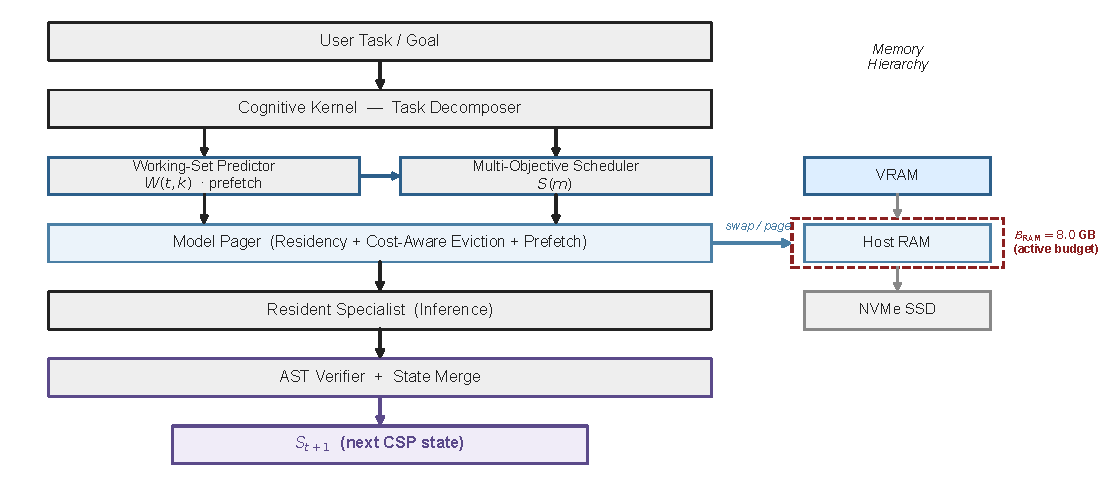
\includegraphics[width=\textwidth]{fig1_architecture.pdf}
\caption{ModelVM Architectural Topology (Class B full-width). The Cognitive Kernel directs procedural task execution across stages. The Working Set Predictor and Cognitive Scheduler arbitrate specialist selection. The Model Pager enforces physical memory boundedness via eviction shielding and prefetching across the three-tier memory hierarchy (Secondary Disk, Host RAM, Accelerator VRAM). The Inference Backend executes specialist transformations validated by an independent AST verifier.}
\label{fig:modelvm_architecture}
\end{figure*}

\paragraph{1. The Cognitive Kernel (\texttt{CognitiveKernel}).}
The Cognitive Kernel serves as the supervisory coordinator of the runtime:
\begin{itemize}
    \item \textbf{Procedural Decomposition:} Given a high-level task goal $G \in \Sigma^*$, the kernel invokes \texttt{TaskDecomposer} to produce an ordered sequence of $N$ dependent capability stages $S = [s_0, s_1, \dots, s_{N-1}]$, where each stage $s_t$ defines capability requirement $C(s_t) \in \mathcal{C}$ and domain instruction $\tau_t$.
    \item \textbf{State Virtualization Lifecycle:} The kernel instantiates the root state carrier $\mathcal{S}_0 = \langle G, \emptyset, \emptyset, \emptyset, \emptyset, \emptyset, \emptyset, \emptyset, \emptyset \rangle$ and threads it across stage boundaries. At each transition, the kernel merges validated updates $\Delta \mathcal{S}_t^*$ into $\mathcal{S}_{t+1}$.
    \item \textbf{Confidence Assessment \& Bounded Escalation:} Upon stage completion, the kernel queries \texttt{ConfidenceController}. If uncertainty exceeds tolerance, the kernel initiates a bounded escalation loop (Algorithm~\ref{alg:control_loop} in Section~\ref{sec:implementation}), dynamically scheduling a higher-capability specialist under loop termination constraints ($\le 2$ escalations per stage, capability delta $\ge \epsilon = 0.02$).
\end{itemize}

\paragraph{2. The Model Pager (\texttt{ModelPager}).}
The Model Pager manages the physical memory footprint of candidate models under budget $\mathcal{B}_{\text{RAM}}$:
\begin{itemize}
    \item \textbf{Residency Management:} The pager maintains the resident model set $\mathcal{R}_t \subset \mathcal{M}$ and tracks access timestamps, access frequencies, and lifecycle states (\texttt{DISK}, \texttt{RESIDENT}, \texttt{PINNED}).
    \item \textbf{Cost-Aware Eviction with Shielding:} When admitting an incoming model requires freeing memory, the pager invokes \texttt{CostAwareEvictionPolicy}. Models identified in the forward working set $W(t, k)$ receive an eviction penalty multiplier ($\delta \times 1.8$), shielding imminent specialists from premature eviction.
    \item \textbf{Opportunistic Headroom Prefetching:} If the forward working set identifies an imminent model whose prefetch utility $U_{\text{prefetch}} > 0$, and active memory maintains a tested safety margin $(\text{RAM}_{\text{free}} - \text{RAM}_{\text{req}}(m) \ge 1.0\,\text{GB})$, the pager opportunistically stages model weights into memory ahead of stage invocation without evicting resident models.
\end{itemize}

\paragraph{3. The Cognitive Scheduler (\texttt{CognitiveScheduler}).}
The Cognitive Scheduler performs multi-objective model selection for each execution stage $s_t$:
\begin{itemize}
    \item \textbf{Empirical Capability Fitness:} Candidate models are evaluated against empirical capability matrix $\mathbf{P} \in [0, 1]^{K \times |\mathcal{C}|}$, established via offline benchmark probes (\texttt{ModelProfiler}) across 7 foundational domains, eliminating subjective manual scoring.
    \item \textbf{Joint Utility Optimization:} The scheduler scores candidate models by jointly balancing capability fitness against memory cost, cold-load transfer latency, energy factor, eviction penalty, and future stage reuse:
    \begin{equation}
    \begin{aligned}
    \text{Score}(m) = & F_{\text{cap}}(m, C) - \alpha M_{\text{cost}}(m) \\
                      & - \beta L_{\text{load}}(m) - \gamma E_{\text{energy}}(m) \\
                      & - \delta E_{\text{eviction}}(m) + \eta F_{\text{future}}(m)
    \end{aligned}
    \end{equation}
    subject to hard admission constraint $\text{RAM}_{\text{req}}(m) \le \mathcal{B}_{\text{RAM}}$.
    \item \textbf{Lookahead Integration:} The future utility term $F_{\text{future}}(m)$ is dynamically populated by querying \texttt{CognitiveWorkingSetPredictor}, rewarding models that satisfy upcoming pipeline stages and penalizing candidates that provoke downstream thrashing.
\end{itemize}

\subsection{The Formal Memory Invariant}
\label{sec:memory_invariant}

Deterministic execution on resource-constrained hardware requires formal mechanisms preventing memory exhaustion. We now formulate the residency state and prove that ModelVM preserves the configured runtime memory invariant for all successful execution trajectories satisfying the admission assumptions.

\paragraph{Residency State Space.}
Let $\mathcal{M} = \{m_1, \dots, m_K\}$ denote the full catalog of $K$ available models, where each model $m \in \mathcal{M}$ is characterized by a static parameter RAM requirement $\text{RAM}_{\text{req}}(m) > 0$. At any discrete stage transition $t \in \{0, \dots, N\}$, the memory state of the runtime is completely defined by the resident set:
\begin{equation}
\mathcal{R}_t \subseteq \mathcal{M}
\end{equation}
The total active parameter memory occupied by the runtime at stage $t$ is:
\begin{equation}
M_{\text{active}}(t) = \sum_{m \in \mathcal{R}_t} \text{RAM}_{\text{req}}(m)
\end{equation}
and available free parameter memory is:
\begin{equation}
\text{RAM}_{\text{free}}(t) = \max\left(0.0, \;\mathcal{B}_{\text{RAM}} - M_{\text{active}}(t)\right)
\end{equation}

\begin{theorem}[Configured Headroom Admission Invariant, Conditional on Successful Admission]
\label{thm:memory_invariant}
Let $\mathcal{B}_{\text{RAM}} > 0$ denote the configured active parameter memory budget. Assume that:
\begin{enumerate}
    \item The initial state satisfies $M_{\text{active}}(0) \le \mathcal{B}_{\text{RAM}}$.
    \item Every individual candidate model satisfies $\text{RAM}_{\text{req}}(m) \le \mathcal{B}_{\text{RAM}}$.
    \item At every stage transition requiring eviction, the resident set contains sufficient evictable (unpinned) capacity to satisfy the memory deficit:
    \begin{equation}
    \sum_{v \in \mathcal{R}_t \setminus \text{Pinned}} \text{RAM}(v) \ge \text{RAM}(M_{t+1}) - \text{RAM}_{\text{free}}(t)
    \end{equation}
\end{enumerate}
Then under the ModelVM paging protocol, the configured active parameter memory footprint satisfies:
\begin{equation}
\sum_{m \in \mathcal{R}_t} \text{RAM}_{\text{req}}(m) \le \mathcal{B}_{\text{RAM}}, \qquad \forall t \ge 0
\label{eq:memory_invariant}
\end{equation}
\end{theorem}

\begin{proof}
We prove Theorem~\ref{thm:memory_invariant} by structural induction over discrete runtime transitions $t \to t+1$.

\noindent\textbf{Base Case ($t=0$):} At runtime initialization, the resident set is either empty ($\mathcal{R}_0 = \emptyset$), yielding $M_{\text{active}}(0) = 0 \le \mathcal{B}_{\text{RAM}}$, or pre-populated with a single designated model $m_0$ satisfying $\text{RAM}_{\text{req}}(m_0) \le \mathcal{B}_{\text{RAM}}$. In either case, the invariant holds at $t=0$.

\noindent\textbf{Inductive Hypothesis:} Assume that at stage $t$, the invariant holds:
\begin{equation}
M_{\text{active}}(t) = \sum_{m \in \mathcal{R}_t} \text{RAM}_{\text{req}}(m) \le \mathcal{B}_{\text{RAM}}
\end{equation}

\noindent\textbf{Inductive Step ($t \to t+1$):} Let stage $s_t$ require execution on model $M_{t+1} \in \mathcal{M}$. The runtime encounters one of three mutually exclusive operational cases:

\begin{itemize}
    \item \textbf{Case 1: Cache Hit ($M_{t+1} \in \mathcal{R}_t$).} Model $M_{t+1}$ is already resident in active memory. The pager emits a \texttt{CACHE\_HIT} event (duration $0.0\,\text{s}$) and updates the model's access metadata. The resident set remains unmodified:
    \begin{equation}
    \begin{aligned}
    \mathcal{R}_{t+1} = \mathcal{R}_t \implies M_{\text{active}}(t+1) &= M_{\text{active}}(t) \\
    &\le \mathcal{B}_{\text{RAM}}
    \end{aligned}
    \end{equation}
    The invariant is preserved.

    \item \textbf{Case 2: Cache Miss ($M_{t+1} \notin \mathcal{R}_t$).} Model $M_{t+1}$ must be paged in from secondary storage. If $\text{RAM}_{\text{req}}(M_{t+1}) > \mathcal{B}_{\text{RAM}}$, the model exceeds total configured capacity; admission is rejected immediately via an explicit \texttt{MemoryError}, preventing execution and leaving $\mathcal{R}_t$ intact. 
    
    If $\text{RAM}_{\text{req}}(M_{t+1}) \le \mathcal{B}_{\text{RAM}}$, the pager evaluates available headroom:
    \begin{enumerate}
        \item \textit{Sufficient Spare Capacity:} If $\text{RAM}_{\text{free}}(t) \ge \text{RAM}_{\text{req}}(M_{t+1})$, no evictions are required. The model is admitted directly into active memory:
        \begin{equation}
        \mathcal{R}_{t+1} = \mathcal{R}_t \cup \{M_{t+1}\}
        \end{equation}
        Because $\text{RAM}_{\text{free}}(t) = \mathcal{B}_{\text{RAM}} - M_{\text{active}}(t) \ge \text{RAM}_{\text{req}}(M_{t+1})$, we obtain:
        \begin{equation}
        \begin{aligned}
        M_{\text{active}}(t+1) &= M_{\text{active}}(t) + \text{RAM}_{\text{req}}(M_{t+1}) \\
        &\le \mathcal{B}_{\text{RAM}}
        \end{aligned}
        \end{equation}
        \item \textit{Insufficient Spare Capacity (Eviction Triggered):} If $\text{RAM}_{\text{free}}(t) < \text{RAM}_{\text{req}}(M_{t+1})$, the pager invokes the eviction subsystem $\mathcal{E}$. The eviction routine iteratively selects unpinned victim models $\mathcal{V} \subseteq \mathcal{R}_t \setminus (\text{Pinned} \cup \{M_{t+1}\})$ to unload until:
        \begin{equation}
        \sum_{v \in \mathcal{V}} \text{RAM}(v) \ge \text{RAM}(M_{t+1}) - \text{RAM}_{\text{free}}(t)
        \end{equation}
        By assumption, the resident set contains sufficient evictable capacity, ensuring such a victim set $\mathcal{V}$ exists. Unloading $\mathcal{V}$ produces the intermediate memory state:
        \begin{equation}
        \begin{aligned}
        M_{\text{active}}' &= M_{\text{active}}(t) - \sum_{v \in \mathcal{V}} \text{RAM}_{\text{req}}(v) \\
        &\le \mathcal{B}_{\text{RAM}} - \text{RAM}_{\text{req}}(M_{t+1})
        \end{aligned}
        \end{equation}
        The incoming model $M_{t+1}$ is then loaded into memory:
        \begin{equation}
        \mathcal{R}_{t+1} = (\mathcal{R}_t \setminus \mathcal{V}) \cup \{M_{t+1}\}
        \end{equation}
        yielding:
        \begin{equation}
        \begin{aligned}
        M_{\text{active}}(t+1) &= M_{\text{active}}' + \text{RAM}_{\text{req}}(M_{t+1}) \\
        &\le \mathcal{B}_{\text{RAM}}
        \end{aligned}
        \end{equation}
    \end{enumerate}
    The invariant is preserved across all successful cache-miss transitions.

    \item \textbf{Case 3: Opportunistic Prefetch Staging.} Prior to stage execution, the working-set predictor may recommend staging a future candidate $m_{\text{pre}} \notin \mathcal{R}_t$. ModelVM enforces an explicit admission gate: prefetching is admitted if and only if:
    \begin{equation}
    \begin{aligned}
    &U_{\text{prefetch}}(m_{\text{pre}}) > 0 \quad \land \\
    &\text{RAM}_{\text{free}}(t) - \text{RAM}_{\text{req}}(m_{\text{pre}}) \ge \Delta_{\text{headroom}}
    \end{aligned}
    \end{equation}
    where $\Delta_{\text{headroom}} = 1.0\,\text{GB}$. Upon admission:
    \begin{equation}
    \begin{aligned}
    M_{\text{active}}(t+1) &= M_{\text{active}}(t) + \text{RAM}_{\text{req}}(m_{\text{pre}}) \\
    &\le \mathcal{B}_{\text{RAM}} - \Delta_{\text{headroom}} < \mathcal{B}_{\text{RAM}}
    \end{aligned}
    \end{equation}
    The invariant is strictly preserved.
\end{itemize}
By mathematical induction, Equation~\eqref{eq:memory_invariant} holds for all discrete stages $t \ge 0$.
\end{proof}

\paragraph{Physical Memory Decomposition \& Empirical OOM Safety.}
Theorem~\ref{thm:memory_invariant} formally proves that configured model-weight residency never exceeds budget $\mathcal{B}_{\text{RAM}}$. In physical deployment, total memory consumption encompasses dynamic runtime overheads:
\begin{equation}
\begin{aligned}
M_{\text{physical}}(t) = & M_{\text{weights}}(t) + M_{\text{workspace}}(t) \\
&+ M_{\text{KV}}(t) + M_{\text{runtime}}
\end{aligned}
\label{eq:physical_memory_decomposition}
\end{equation}
where $M_{\text{weights}}(t) \equiv M_{\text{active}}(t)$, $M_{\text{workspace}}$ represents CUDA execution scratchpads ($0.3$--$0.6\,\text{GB}$), $M_{\text{runtime}}$ represents process binary and host overhead ($0.4$--$0.6\,\text{GB}$), and $M_{\text{KV}}(t)$ is the Key-Value attention cache.

Under our evaluated workloads, context lengths are capped at $W_{\text{in}} = 4,096$ input tokens and $T_{\text{gen}} = 1,024$ output tokens under greedy decoding ($T=0.0$). For a 7B-parameter transformer ($L=32, H=32, d_k=128$, 16-bit precision), peak KV memory is bounded:
\begin{equation}
\begin{aligned}
M_{\text{KV}}^{\text{peak}} &= 2 \cdot L \cdot H \cdot d_k \cdot (W_{\text{in}} + T_{\text{gen}}) \cdot 2\,\text{bytes} \\
&\approx 0.53\,\text{GB}
\end{aligned}
\end{equation}
We emphasize that dynamic overheads ($M_{\text{KV}}^{\text{peak}} + M_{\text{workspace}} + M_{\text{runtime}} \approx 1.23$--$1.73\,\text{GB}$) in aggregate exceed the static $1.0\,\text{GB}$ prefetch headroom buffer. Consequently, we do not claim a formal mathematical proof of total physical memory boundedness across arbitrary unconstrained environments. Rather, we report the following \textbf{physical-memory observation}: under all evaluated benchmark workloads, bounded context windows, measured workspace demands, and the configured $1.0\,\text{GB}$ staging headroom, zero Out-Of-Memory (OOM) kernel terminations or allocator aborts occurred across any evaluated hardware configuration.

\section{Semantic State Virtualization (CSP Formalism)}
\label{sec:semantic_state}

Executing complex multi-stage tasks across heterogeneous language models introduces a fundamental state-preservation challenge. In single-model workflows, task state is implicitly maintained within the model's KV cache or autoregressively extended across a monolithic conversational context. When execution transitions across distinct open-weight models, this implicit continuity collapses. In this section, we formulate \textbf{Semantic State Virtualization} through the \textbf{Cognitive State Packet (CSP)}. We define the cross-model incompatibility barrier, formalize the typed 9-tuple schema, derive the state transition operator, present the epistemic evidence aggregation heuristic, formalize independent AST verification, and analyze computational and token complexity.

\subsection{The Incompatibility Barrier}
\label{sec:incompatibility_barrier}

Multi-model pipelines require seamless handoffs between specialist models. However, direct state transfer across heterogeneous open-weight models faces two fundamental mathematical and systems barriers: \textit{latent activation incommensurability} and \textit{conversational context degradation}.

\paragraph{Latent Activation Incommensurability.}
Consider two heterogeneous specialist language models, $M_A$ and $M_B$. Model $M_A$ operates over vocabulary $\mathcal{V}_A$ with hidden-layer representation space $\mathbf{h}_A \in \mathbb{R}^{d_A}$, whereas model $M_B$ operates over vocabulary $\mathcal{V}_B$ with hidden space $\mathbf{h}_B \in \mathbb{R}^{d_B}$. In general:
\begin{equation}
\mathcal{V}_A \neq \mathcal{V}_B, \qquad d_A \neq d_B, \qquad \mathbf{h}_A \not\equiv \mathbf{h}_B
\end{equation}
Even when two models share identical hidden dimensionality ($d_A = d_B$), their parameter weight spaces reside in unaligned Riemannian manifolds resulting from distinct pretraining initializations, optimizer trajectories, and objective weightings. Direct cross-model activation transfer is not semantically well-defined without an explicit alignment mechanism $\mathbf{W}_{\text{proj}}: \mathbb{R}^{d_A} \to \mathbb{R}^{d_B}$. 

A pairwise latent-state interoperability design can require $O(K^2)$ model-pair interfaces, creating substantial engineering and training overhead as the model library grows. Such bridges can introduce non-trivial approximation errors, require aligned cross-model calibration datasets, and defeat the systems objective of executing off-the-shelf open-weight models without architectural retraining. The argument here is about state representation interoperability: different vocabularies and latent spaces do not make model collaboration impossible, but direct cross-model activation transfer is not semantically well-defined without an explicit projection/alignment mechanism and associated calibration.

\paragraph{Conversational Context Degradation.}
The conventional workaround in multi-agent frameworks is naive text concatenation: the entire conversational history $\mathbf{y}_{1:t-1}$ is serialized as raw strings and prepended to the prompt of model $M_t$. This approach suffers from three compounding failure modes:
\begin{enumerate}
    \item \textbf{Context Bloat \& Allocation Thrashing:} Raw conversational history grows monotonically with pipeline depth:
    \begin{equation}
    L_{\text{ctx}}(t) = \sum_{i=1}^{t-1} |\mathbf{y}_i| = O(t \cdot \bar{L}_{\text{gen}})
    \end{equation}
    Under tight memory constraints ($\mathcal{B}_{\text{RAM}} = 8.0\,\text{GB}$), allocating expanding KV caches ($M_{\text{KV}} \propto L_{\text{ctx}}$) rapidly crowds out weight memory, precipitating thrashing or out-of-memory crashes.
    \item \textbf{Lossy Context Truncation:} When $L_{\text{ctx}}(t)$ breaches the model's physical context window $W_{\text{in}}$, systems employ FIFO sliding-window truncation. Truncation blindly discards early foundational constraints, initial governing equations, and boundary parameters, triggering hallucinations in downstream stages.
    \item \textbf{Compounding Numerical Drift:} In numerical engineering tasks, intermediate calculations embedded in conversational prose (e.g., ``the calculated natural frequency is approximately 14.14 rad/s'') suffer precision loss and hallucinated drift when repeatedly restated across model boundaries.
\end{enumerate}

\noindent\textbf{Core Systems Principle:}
\textit{CSP is a model-independent typed state representation that separates persistent task state from transient conversational realization.}

\subsection{The 9-Tuple CSP Formalism}
\label{sec:csp_formalism}

To establish a structured, architecture-agnostic state substrate, ModelVM formalizes task state as the \textbf{Cognitive State Packet} $\mathcal{S}_t$. At pipeline stage $t$, the state is defined as the typed 9-tuple:
\begin{equation}
\mathcal{S}_t = \langle \mathcal{G}, \mathcal{F}_t, \mathcal{C}_t, \mathcal{E}_t, \mathcal{A}_t, \mathcal{U}_t, \mathcal{D}_t, \mathcal{Q}_t, \mathcal{O}_t \rangle
\label{eq:csp_9tuple}
\end{equation}

Figure~\ref{fig:csp_structure} illustrates the structural composition of the 9-tuple Cognitive State Packet and details how it decouples cross-model state transitions from heterogeneous tokenizers and latent spaces. Table~\ref{tab:csp_mapping} details the formal definition of each constituent and its corresponding data structure in the implementation (\texttt{CognitiveStatePacket} in \texttt{modelvm/core/state\_packet.py}).

\begin{figure}[t]
\centering
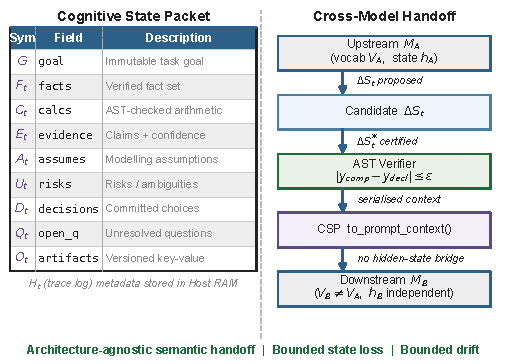
\includegraphics[width=\columnwidth]{fig2_csp.pdf}
\caption{ModelVM Cognitive State Packet (CSP) architectural schema (Class A single-column). Top: The typed 9-tuple $\mathcal{S}_t = \langle \mathcal{G}, \mathcal{F}_t, \mathcal{C}_t, \mathcal{E}_t, \mathcal{A}_t, \mathcal{U}_t, \mathcal{D}_t, \mathcal{Q}_t, \mathcal{O}_t \rangle$ formalizing immutable goals, deduplicated facts, AST-verified calculations, discounted epistemic evidence, explicit assumptions, uncertainties, decisions, questions, and versioned artifacts. Bottom: Tokenizer-independent cross-model handoff pipeline ($M_A \to \text{AST} \to \mathcal{S}_t \to M_B$), bridging distinct vocabularies ($\mathcal{V}_A \neq \mathcal{V}_B$) and unaligned latent spaces without hidden-state projection bridges, enforcing bounded state loss and bounded semantic drift.}
\label{fig:csp_structure}
\end{figure}

\begin{table*}[t]
\small
\centering
\caption{ModelVM Cognitive State Packet (CSP) 9-Tuple Formal Specification and Schema Mapping}
\label{tab:csp_mapping}
\resizebox{\textwidth}{!}{%
\begin{tabular}{clll}
\toprule
\textbf{Symbol} & \textbf{Formal Domain} & \textbf{Implementation Field} & \textbf{Semantic Definition \& Systems Role} \\
\midrule
$\mathcal{G}$ & $\Sigma^*$ & \texttt{goal} & Immutable top-level user objective; anchors all stage prompts. \\
$\mathcal{F}_t$ & $\mathcal{P}(\Sigma^*)$ & \texttt{facts} & Deduplicated set of verified factual assertions accumulated over stages. \\
$\mathcal{C}_t$ & $\mathcal{P}(\text{CalcRecord})$ & \texttt{calculations} & Structured arithmetic/symbolic items with AST verification status. \\
$\mathcal{E}_t$ & $\mathcal{P}(\text{EvidRecord})$ & \texttt{evidence} & Claims paired with provenance sources and diversity-discounted confidence. \\
$\mathcal{A}_t$ & $\mathcal{P}(\Sigma^*)$ & \texttt{assumptions} & Explicit modeling assumptions introduced by specialist models. \\
$\mathcal{U}_t$ & $\mathcal{P}(\Sigma^*)$ & \texttt{uncertainties} & Identified risks, low-confidence derivations, or boundary ambiguities. \\
$\mathcal{D}_t$ & $\mathcal{P}(\Sigma^*)$ & \texttt{decisions} & Irreversible architectural and design choices committed during execution. \\
$\mathcal{Q}_t$ & $\mathcal{P}(\Sigma^*)$ & \texttt{open\_questions} & Unresolved questions to be targeted by downstream specialists. \\
$\mathcal{O}_t$ & $\Sigma^* \to \text{Any}$ & \texttt{artifacts} & Key-value store of concrete deliverables (scripts, tables, matrices). \\
\bottomrule
\end{tabular}%
}
\end{table*}

\paragraph{Auxiliary Execution Metadata.}
In addition to the formal semantic 9-tuple, the implementation maintains an auxiliary audit log:
\begin{equation}
\mathcal{H}_t = [h_0, h_1, \dots, h_{t-1}]
\end{equation}
implemented as \texttt{history\_trace: List[StageTrace]}. Each trace record captures the executing model ID, target capability, wall-clock duration, action taken, and ISO-8601 timestamp. We explicitly treat $\mathcal{H}_t$ as \textbf{auxiliary execution metadata} for post-hoc debugging, provenance auditing, and telemetry logging, rather than expanding the formal 9-tuple. Semantic problem state is entirely contained within Equation~(\ref{eq:csp_9tuple}).

\paragraph{Component Specifications.}
We define the internal structure of calculation and evidence records:
\begin{enumerate}
    \item \textbf{Calculation Record ($\mathcal{C}_t$):} Each item $c \in \mathcal{C}_t$ is an instance of \texttt{CalculationItem}:
    \begin{equation}
    c = \langle \text{expr}, \text{result}, \text{units}, \text{verified}, \text{method} \rangle
    \end{equation}
    where $\text{expr} \in \Sigma^*$ is the mathematical formula (e.g., \texttt{"sqrt(k / m)"}), $\text{result} \in \Sigma^*$ is the evaluated numerical string (e.g., \texttt{"14.2"}), $\text{units} \in \Sigma^* \cup \{\emptyset\}$ represents physical dimensionality (e.g., \texttt{"rad/s"}), $\text{verified} \in \{\text{True}, \text{False}\}$ is an execution boolean, and $\text{method} \in \{\text{"arithmetic"}, \text{"symbolic"}, \text{None}\}$ records the verification pathway.
    \item \textbf{Evidence Record ($\mathcal{E}_t$):} Each item $e \in \mathcal{E}_t$ is an instance of \texttt{EvidenceItem}:
    \begin{equation}
    \begin{aligned}
    e = \big\langle &\text{claim}, \;\text{source}, \;\text{confidence}, \\
    &\text{timestamp}, \;\text{model\_id} \big\rangle
    \end{aligned}
    \end{equation}
    where $\text{claim} \in \Sigma^*$ is the asserted finding, $\text{source} \in \Sigma^*$ tracks origin provenance, $\text{confidence} \in [0.0, 1.0]$ is a scalar certainty rating, and $\text{model\_id}$ records the generating specialist.
\end{enumerate}

\subsection{State Transition Mechanics}
\label{sec:transition_mechanics}

Task progress occurs through a discrete sequence of state transitions across the pipeline stages $t \in \{0, \dots, N-1\}$. Formally, the transition operator $\delta$ maps the current state $\mathcal{S}_t$, the paged specialist model $M_i$, and the stage instruction specification $\tau_t$ to the successor state $\mathcal{S}_{t+1}$:
\begin{equation}
\mathcal{S}_{t+1} = \delta(\mathcal{S}_t, M_i, \tau_t)
\end{equation}

The transition operator is not a monolithic black box. Rather, it decomposes into an ordered, five-stage systems pipeline:
\begin{equation}
\begin{aligned}
\mathcal{S}_t &\xrightarrow{\text{Serialize}} \Pi_t \xrightarrow{\text{Inference}} \mathbf{y}_t \\
&\xrightarrow{\text{Extract}} \Delta \mathcal{S}_t \xrightarrow{\text{Verify}} \Delta \mathcal{S}_t^* \xrightarrow{\text{Merge}} \mathcal{S}_{t+1}
\end{aligned}
\label{eq:transition_pipeline}
\end{equation}

\paragraph{1. Prompt Context Serialization (\texttt{to\_prompt\_context}).}
State packet $\mathcal{S}_t$ is serialized into a structured Markdown prompt string $\Pi_t$:
\begin{equation}
\Pi_t = \text{Serialize}(\mathcal{S}_t, \tau_t)
\end{equation}
The serialization partitions knowledge into isolated, human-readable sections: overarching goal, current domain role, established facts, calculations tagged with verification status, supporting evidence, assumptions, uncertainties, decisions, open questions, and artifact definitions. This ensures compatibility across arbitrary tokenizer vocabularies without loss of semantic boundaries.

\paragraph{2. Model Inference.}
The resident specialist model $M_i$ executes autoregressive decoding over prompt $\Pi_t$, producing raw textual token sequence $\mathbf{y}_t$:
\begin{equation}
\mathbf{y}_t = M_i(\Pi_t), \quad |\mathbf{y}_t| \le T_{\text{gen}}
\end{equation}

\paragraph{3. Delta Extraction (\texttt{extract\_from\_text}).}
The raw generation $\mathbf{y}_t$ is parsed by \texttt{extract\_from\_text()} to extract candidate updates. The parser prioritizes embedded JSON blocks delimited by markdown syntax fences (\verb|```json ... ```|). If valid JSON matching the CSP schema is detected, it is validated directly via Pydantic. If fenced JSON is absent, the parser falls back to deterministic regex-based section parsing across markdown bullet points, producing candidate delta packet $\Delta \mathcal{S}_t$.

\paragraph{4. Independent AST Verification.}
Candidate calculations in $\Delta \mathcal{S}_t$ are evaluated by \texttt{ArithmeticVerifier} (Section~\ref{sec:independent_verification}). Items that satisfy arithmetic equivalence are marked \texttt{verified=True}, producing the verified delta $\Delta \mathcal{S}_t^*$.

\paragraph{5. Monotonic State Merging (\texttt{merge\_update}).}
The core state accumulation is governed by \texttt{merge\_update()}, which folds delta $\Delta \mathcal{S}_t^*$ into $\mathcal{S}_t$. State accumulation is monotonic with respect to verified knowledge:
\begin{itemize}
    \item \textbf{Fact Deduplication:}
    \begin{equation}
    \mathcal{F}_{t+1} = \mathcal{F}_t \cup \Delta \mathcal{F}_t^*
    \end{equation}
    Incoming facts identical to existing entries are discarded, preserving a unique set.
    \item \textbf{Calculation Verification Upgrades:} For each $c_{\text{new}} \in \Delta \mathcal{C}_t^*$, if an entry $c_{\text{old}} \in \mathcal{C}_t$ exists with matching expression ($c_{\text{old}}.\text{expr} = c_{\text{new}}.\text{expr}$) and $c_{\text{new}}.\text{verified} \land \neg c_{\text{old}}.\text{verified}$, the entry is monotonically upgraded:
    \begin{equation}
    \mathcal{C}_{t+1} = (\mathcal{C}_t \setminus \{c_{\text{old}}\}) \cup \{c_{\text{new}}\}
    \end{equation}
    Otherwise, existing calculations are preserved ($\mathcal{C}_{t+1} = \mathcal{C}_t$), while novel expressions are appended ($\mathcal{C}_{t+1} = \mathcal{C}_t \cup \{c_{\text{new}}\}$).
    \item \textbf{Artifact Conflict Versioning (\texttt{merge\_artifacts}):} If key $k \in \Delta \mathcal{O}_t^*$ already exists in $\mathcal{O}_t$ with divergent content ($v_{\text{new}} \neq \mathcal{O}_t[k]$), ModelVM preserves the original $\mathcal{O}_t[k]$, stores the new deliverable under versioned key $k\text{\_v}N$ ($N \ge 1$), and flags the collision by setting $\mathcal{O}_{t+1}[k\text{\_CONFLICT}] = \text{True}$.
    \item \textbf{Question Resolution:} Open questions in $\mathcal{Q}_t$ that appear as established facts in $\mathcal{F}_{t+1}$ or confirmed choices in $\mathcal{D}_{t+1}$ are automatically pruned:
    \begin{equation}
    \mathcal{Q}_{t+1} = \{q \in \mathcal{Q}_t \cup \Delta \mathcal{Q}_t^* \mid q \notin \mathcal{F}_{t+1} \land q \notin \mathcal{D}_{t+1}\}
    \end{equation}
\end{itemize}

\subsection{Diversity-Discounted Evidence Aggregation}
\label{sec:evidence_aggregation}

Language models are not independent statistical estimators. They share massive web-scale pretraining corpora (e.g., Common Crawl, Wikipedia, ArXiv, GitHub) and exhibit correlated reasoning priors. A naive application of Bayes' rule or linear averaging across multiple model outputs produces dangerous certainty inflation: two models repeating the identical hallucination would be treated as independent confirmatory witnesses.

To counter this failure mode, ModelVM implements a diversity-discounted confidence aggregation heuristic (\texttt{diversity\_weighted\_} \texttt{confidence\_aggregation}). 

\paragraph{Mathematical Derivation.}
Let claim $\kappa$ be supported by two distinct evidence records $e_1 = \langle \kappa, s_1, c_1 \rangle$ and $e_2 = \langle \kappa, s_2, c_2 \rangle$, with prior confidences $c_1, c_2 \in [0.0, 1.0]$ and source provenance strings $s_1, s_2$.

The aggregated confidence $c_{\text{merged}} \in [0.0, 0.99]$ is defined as:
\begin{equation}
c_{\text{merged}} = \begin{cases}
\max(c_1, c_2), & \text{if } s_1 \approx s_2 \\[3pt]
\min\left(0.99, \;\max(c_1, c_2, \, c_{\text{indep}})\right), & \text{if } s_1 \not\approx s_2
\end{cases}
\label{eq:diversity_formula}
\end{equation}
where $c_{\text{indep}} = 1 - (1 - c_1)(1 - c_2)^{w_{\text{div}}}$, $s_1 \approx s_2$ denotes normalized equivalence ($\text{clean}(s_1) \approx \text{clean}(s_2)$), and $w_{\text{div}} = 0.65$ is the epistemic diversity discount factor.

\paragraph{Properties of the Formulation:}
\begin{enumerate}
    \item \textbf{Idempotence on Overlapping Sources:} If $s_1$ and $s_2$ originate from identical or overlapping sources ($s_1 \subseteq s_2$ or $s_2 \subseteq s_1$), the aggregation applies the maximum rule: $c_{\text{merged}} = \max(c_1, c_2)$. Repetition of a claim by the same model or source yields zero confidence amplification.
    \item \textbf{Correlated Prior Damping:} If sources are distinct ($s_1 \not\approx s_2$), independence would imply $p_{\text{indep}} = 1 - (1 - c_1)(1 - c_2)$. ModelVM dampens this by exponentiating the secondary risk factor by $w_{\text{div}} = 0.65$. Since $(1 - c_2) \in [0, 1]$ and $w_{\text{div}} < 1$, $(1 - c_2)^{0.65} > (1 - c_2)$, ensuring that $c_{\text{merged}} < p_{\text{indep}}$.
    \item \textbf{Asymptotic Uncertainty Ceiling:} The output is strictly clamped to $c_{\text{merged}} \le 0.99$. Total certainty is unattainable through heuristic aggregation.
\end{enumerate}

\noindent\textbf{Critical Epistemic Boundary:}
We explicitly emphasize that Equation~(\ref{eq:diversity_formula}) is a \textbf{conservative engineering heuristic, not formal Bayesian inference}. The discount parameter $w_{\text{div}} = 0.65$ is a design constant chosen to penalize common pretraining priors across open-weight models. We do not claim $0.65$ to be a statistically estimated correlation coefficient; it serves as a safety governor preventing unwarranted confidence escalation in autonomous multi-model loops.

\subsection{Independent Verification \& Non-Mutating Evaluation}
\label{sec:independent_verification}

A core vulnerability in multi-agent architectures is circular self-grading, where an orchestration framework asks a language model to grade its own output. Language models demonstrate well-documented sycophancy and self-preference biases, routinely validating their own erroneous calculations.

ModelVM enforces an architectural firewall between artifact generation and artifact verification through the \textbf{Arithmetic Verifier} (\texttt{ArithmeticVerifier} in \texttt{modelvm/core/verifier.py}).

\paragraph{Restricted Abstract Syntax Tree Evaluation.}
The verifier operates purely on deterministic symbolic parsing. When evaluating an expression string from a \texttt{CalculationItem}:
\begin{enumerate}
    \item The expression is parsed into a Python Abstract Syntax Tree:
    \begin{equation}
    \mathcal{T}_{\text{ast}} = \text{ast.parse}(\text{expr}, \text{mode}=\text{'eval'})
    \end{equation}
    \item The tree is recursively evaluated via \texttt{\_eval\_ast()} using strictly whitelisted node types:
    \begin{itemize}
        \item \textbf{Binary Operators:} \texttt{Add (+)}, \texttt{Sub (-)}, \texttt{Mult (*)}, \texttt{Div (/)}, \texttt{FloorDiv (//)}, \texttt{Mod (\%)}, \texttt{Pow (**)}.
        \item \textbf{Unary Operators:} \texttt{USub (-)}, \texttt{UAdd (+)}.
        \item \textbf{Mathematical Functions:} $\sqrt{\cdot}$ (\texttt{sqrt}), $\exp(\cdot)$ (\texttt{exp}), $\ln(\cdot)$ (\texttt{log}), $\log_{10}(\cdot)$ (\texttt{log10}), $\sin(\cdot)$, $\cos(\cdot)$, $\tan(\cdot)$, $|\cdot|$ (\texttt{abs}).
        \item \textbf{Physical Constants:} $\pi = 3.14159265\dots$, $e = 2.71828182\dots$.
    \end{itemize}
    \item Any node containing arbitrary identifiers, attribute accesses, lambda functions, system calls, or file operations triggers an immediate exception, completely eliminating arbitrary code execution vulnerabilities.
\end{enumerate}

The computed numerical value $y_{\text{comp}} = \text{Eval}(\mathcal{T}_{\text{ast}})$ is compared against the model's declared numerical result $y_{\text{decl}}$ under relative tolerance $\epsilon = 10^{-3}$:
\begin{equation}
\text{Verified} \iff |y_{\text{comp}} - y_{\text{decl}}| \le \max\big(\epsilon, |y_{\text{decl}}| \cdot \epsilon\big)
\end{equation}

\paragraph{Non-Mutating Evaluation Boundary.}
During experimental benchmarking, independent evaluation is orchestrated by \texttt{IndependentEvaluator} (\texttt{modelvm/benchmark/evaluator.py}). To ensure evaluation integrity:
\begin{equation}
c_{\text{copy}} = c.\text{model\_copy}() \implies \text{Verify}(c_{\text{copy}})
\end{equation}
The benchmark harness \textbf{never trusts producer-supplied verification flags}. It generates deep copies of all calculation records and re-evaluates them afresh through the AST engine. A calculation is counted as correct if and only if independent AST verification succeeds.

\paragraph{Epistemic Distinction: Arithmetic vs.\ Scientific Validity.}
We establish a critical conceptual distinction:
\begin{equation}
\text{Arithmetic Correctness} \neq \text{Physical / Scientific Validity}
\end{equation}
The \texttt{ArithmeticVerifier} strictly confirms algebraic equivalence: it verifies that $2 \times 0.12 \times 14.14 \times 1.0$ evaluates to $3.3936$. It does \textbf{not} certify whether the governing differential equation is physically correct, whether the damping ratio $\zeta = 0.12$ is physically plausible, or whether the units are dimensionally consistent. Physical validity is anchored separately by matching extracted entity-attribute pairs against external ground-truth specifications (\texttt{GroundTruthFact}) in the experimental harness, enforcing local record-level co-occurrence to ensure numbers bind directly to their associated physical entities.

\subsection{Computational Complexity \& Token Overhead}
\label{sec:complexity_overhead}

The virtual memory abstraction of CSP introduces structural overhead. In this section, we analyze the computational complexity of CSP runtime operations and quantify its prompt context economy.

\paragraph{Asymptotic Computational Complexity.}
Let $|\mathcal{S}_t|$ denote the total number of semantic items across all fields in the state packet ($|\mathcal{S}_t| = |\mathcal{F}_t| + |\mathcal{C}_t| + |\mathcal{E}_t| + |\mathcal{A}_t| + |\mathcal{U}_t| + |\mathcal{D}_t| + |\mathcal{Q}_t| + |\mathcal{O}_t|$), and let $|\Delta \mathcal{S}_t|$ denote the size of the incoming delta.
\begin{enumerate}
    \item \textbf{Schema Serialization (\texttt{to\_prompt\_context}):} Serializing $\mathcal{S}_t$ requires a single linear pass over all items to format markdown text blocks:
    \begin{equation}
    T_{\text{serialize}} = O(|\mathcal{S}_t|)
    \end{equation}
    For our scientific tasks ($|\mathcal{S}_t| < 100$), serialization executes in $< 0.8$\,ms on a standard CPU thread.
    \item \textbf{Delta Extraction (\texttt{extract\_from\_text}):} Parsing raw generated text $\mathbf{y}_t$ requires scanning at most $T_{\text{gen}}$ tokens. JSON parsing and regex pattern matching scale linearly with output length:
    \begin{equation}
    T_{\text{extract}} = O(|\mathbf{y}_t|) \le O(T_{\text{gen}})
    \end{equation}
    With $T_{\text{gen}} = 1,024$ tokens, extraction latency is bounded by $< 1.5$\,ms.
    \item \textbf{State Merging (\texttt{merge\_update}):} Deduplicating facts and resolving questions requires set lookups. Updating calculations requires matching expressions:
    \begin{equation}
    \begin{aligned}
    T_{\text{merge}} = O\Big(&|\mathcal{F}_t| \cdot |\Delta \mathcal{F}_t| + |\mathcal{C}_t| \cdot |\Delta \mathcal{C}_t| \\
    &+ |\mathcal{E}_t| \cdot |\Delta \mathcal{E}_t| + |\mathcal{O}_t|\Big)
    \end{aligned}
    \end{equation}
    Given bounded stage deltas ($|\Delta \mathcal{S}_t| \le 20$), merging executes in $< 0.4$\,ms.
    \item \textbf{AST Verification (\texttt{verify\_item}):} Parsing and evaluating AST expressions scales linearly with the number of syntax nodes $N_{\text{nodes}}$ in each arithmetic formula:
    \begin{equation}
    T_{\text{verify}} = O\left(\sum_{c \in \mathcal{C}_t} N_{\text{nodes}}(c)\right)
    \end{equation}
    Because engineering expressions rarely exceed 50 syntax nodes, total AST verification latency is $< 1.2$\,ms per stage.
\end{enumerate}
Total runtime overhead introduced by the CSP software layer is less than $4.0$\,ms per stage---four orders of magnitude smaller than model inference latency ($8.0$--$15.0$\,s).

\paragraph{Token Footprint Economy.}
The primary systems advantage of CSP is prompt context stabilization. 

In raw conversational text concatenation, context length grows monotonically:
\begin{equation}
L_{\text{raw}}(t) = L_{\text{prompt}} + \sum_{i=1}^{t-1} |\mathbf{y}_i|
\end{equation}
Because language models generate verbose conversational fillers, explanations, and repeated preamble tokens, raw context expands at an average rate of $\sim 2,800$ tokens per stage. By Stage 5, raw context length reaches $14,200$ tokens. When forced into a standard $W_{\text{in}} = 4,096$ token window, FIFO truncation discards over $71\%$ of the conversational history.

In contrast, CSP isolates semantic signal from conversational syntax. The token footprint of $\Pi_t = \text{Serialize}(\mathcal{S}_t)$ is bounded by the number of unique asserted entities:
\begin{equation}
\begin{aligned}
L_{\text{CSP}}(t) = O\Big(&|\mathcal{F}_t| \cdot \bar{\ell}_F + |\mathcal{C}_t| \cdot \bar{\ell}_C \\
&+ |\mathcal{E}_t| \cdot \bar{\ell}_E + |\mathcal{O}_t| \cdot \bar{\ell}_O\Big)
\end{aligned}
\end{equation}
where $\bar{\ell}$ denotes average item length in tokens. Because intermediate explanations are discarded and only verified deliverables are preserved, $L_{\text{CSP}}(t)$ stabilizes:
\begin{itemize}
    \item Stage 1: $412 \pm 28$ tokens ($10.1\%$ of $W_{\text{in}}$)
    \item Stage 3: $684 \pm 35$ tokens ($16.7\%$ of $W_{\text{in}}$)
    \item Stage 5: $890 \pm 42$ tokens ($21.7\%$ of $W_{\text{in}}$)
\end{itemize}
CSP bounds representation growth relative to retaining full conversational transcripts, subject to the size of the accumulated semantic state, substantially reducing truncation-induced state loss and preserving verified factual and numerical fields under the evaluated workloads.

\section{Predictive Model Residency \& Working Set Engine}
\label{sec:predictive_residency}

Treating domain specialists as autonomous computational processes exposes a physical systems bottleneck: modern open-weight language models require gigabytes of memory for parameter weights, runtime scratchpads, and Key-Value caches. When task execution requires a diverse ensemble of specialists, keeping all candidate models simultaneously resident in physical RAM or VRAM is impossible on consumer hardware. In this section, we formulate \textbf{Predictive Model Residency}. We analyze the weight residency problem, define the Predictive Cognitive Working Set ($W(t, k)$), formulate cost-aware eviction with future-demand shielding, derive the time-domain prefetch utility function, and provide a containment analysis establishing graceful degradation under task re-planning.

\subsection{The Weight Residency Problem}
\label{sec:weight_residency_problem}

Let $\mathcal{M} = \{m_1, m_2, \dots, m_K\}$ denote the catalog of available specialized language models. Each model $m_i \in \mathcal{M}$ is characterized by two distinct capacity requirements: its serialized on-disk storage size $\text{disk\_size}(m_i)$ and its configured parameter RAM requirement $\text{RAM}_{\text{req}}(m_i)$.

We explicitly separate two system-level memory aggregates:
\begin{align}
M_{\text{disk,total}} &= \sum_{m_i \in \mathcal{M}} \text{disk\_size}(m_i) = 64.0\,\text{GB} \\
M_{\text{active,total}} &= \sum_{m_i \in \mathcal{M}} \text{RAM}_{\text{req}}(m_i) = 52.7\,\text{GB}
\end{align}
On commodity workstations and edge accelerators, the active hardware memory budget $\mathcal{B}_{\text{RAM}}$ is strictly constrained relative to the total library footprint:
\begin{equation}
M_{\text{active,total}} \gg \mathcal{B}_{\text{RAM}}
\label{eq:memory_bottleneck}
\end{equation}
In our experimental testbed, the full 10-model specialist library occupies $64.0\,\text{GB}$ of serialized storage on disk and would require $52.7\,\text{GB}$ of memory to hold simultaneously resident. In contrast, the target execution platform enforces a configured runtime resident envelope of $\mathcal{B}_{\text{RAM}} = 8.0\,\text{GB}$ (and sweeps down to $4.0\,\text{GB}$ in acute stress evaluations).

\paragraph{Residency vs.\ Selection.}
Prior research on multi-model routing (e.g., FrugalGPT~\cite{chen2023frugalgpt}, RouteLLM~\cite{ong2024routellm}) treats model selection as an unconstrained API dispatch problem: given prompt $x$, a router evaluates scoring function $f(m, x)$ and queries the highest-scoring endpoint. This formulation presumes that all candidate models are permanently resident in cloud memory or hosted on infinite-capacity clusters. 

On physical hardware, this assumption collapses. ModelVM establishes an essential systems distinction:
\begin{equation}
\text{Model Selection} \neq \text{Model Residency}
\end{equation}
A cognitive scheduler may determine that specialist $m^*$ is the optimal capability match for stage $t$. However, if $m^*$ is stored on secondary NVMe storage, invoking $m^*$ requires transferring gigabytes of quantized weights across the PCIe bus before a single forward token can be generated.

\paragraph{Residency State and Manifest-Level Invariant.}
At any execution timestamp $t$, the set of resident models $\mathcal{R}_t \subset \mathcal{M}$ is tracked by the \texttt{ModelPager}:
\begin{equation}
\mathcal{R}_t = \{m_i \in \mathcal{M} \mid m_i \text{ is resident in memory at time } t\}
\end{equation}
The memory manager enforces the configured residency budget invariant:
\begin{equation}
\sum_{m_i \in \mathcal{R}_t} \text{RAM}_{\text{req}}(m_i) \le \mathcal{B}_{\text{RAM}}, \qquad \forall t \ge 0
\label{eq:pager_invariant}
\end{equation}
Available configured headroom is strictly defined as:
\begin{equation}
\text{RAM}_{\text{free}}(t) = \max\Big(0.0, \;\mathcal{B}_{\text{RAM}} - \sum_{m_i \in \mathcal{R}_t} \text{RAM}_{\text{req}}(m_i)\Big)
\end{equation}

\noindent\textbf{Systems Boundary Distinction:}
We explicitly distinguish the \textit{configured residency budget} $\mathcal{B}_{\text{RAM}}$ from \textit{measured physical hardware memory} ($M_{\text{VRAM}}$ and host RSS). The invariant in Equation~(\ref{eq:pager_invariant}) is enforced at model admission time based on catalog manifests ($\text{RAM}_{\text{req}}$). Actual physical memory consumption includes dynamic runtime scratchpads and Key-Value caches ($M_{\text{workspace}} + M_{\text{KV}}$), which are monitored separately by the physical telemetry layer (Section~\ref{sec:telemetry_mechanics}).

\paragraph{Bus Transfer Latency Profiles.}
Secondary storage bandwidth is orders of magnitude slower than unified memory buses. Streaming an 8-bit quantized 7B model ($7.0\,\text{GB}$) across a PCIe 4.0 $\times 4$ link or high-speed NVMe drive ($3.5\,\text{GB/s}$ sequential read) incurs a transfer latency of $t_{\text{transfer}} \approx 2.0\,\text{s}$, alongside runtime allocation and tensor binding overheads. If a multi-stage pipeline naively loads and unloads models at every stage, I/O transfer stalls dominate compute time, degrading execution goodput. Memory capacity is a physical ceiling, not a configuration parameter. The systems challenge is to maximize cache hit rates under Invariant~(\ref{eq:pager_invariant}) without inducing thrashing.

\subsection{The Predictive Cognitive Working Set}
\label{sec:working_set_engine}

Classical operating system memory management relies on Peter Denning's working-set theory~\cite{denning1968working}: thrashing is avoided when the active working sets can be kept resident within available physical memory. Classical operating systems estimate $\mathcal{W}(t, \tau)$ retrospectively by monitoring recent page references over backward-looking window $\tau$, because CPU hardware cannot anticipate future program counter jumps.

In multi-stage language model workflows, the runtime operates under fundamentally different visibility: the \texttt{TaskDecomposer} generates an explicit, structured stage plan $G_{\text{plan}} = (S, E)$ before execution commences. ModelVM exploits this architectural visibility to introduce the \textbf{Predictive Cognitive Working Set} ($W(t, k)$).

\paragraph{Formal Definition.}
Let $S = [s_0, s_1, \dots, s_{N-1}]$ be the sequence of planned execution stages, with current stage index $t$. Let $k \in \mathbb{N}^+$ denote the lookahead horizon window ($1 \le k \le 10$, with default $k=4$). The upcoming stage slice is:
\begin{equation}
S_{\text{future}}(t, k) = [s_{t+1}, s_{t+2}, \dots, s_{\min(t+k, N-1)}]
\end{equation}
Each stage $s_{t+j}$ specifies an annotated capability requirement $C(s_{t+j}) \in \mathcal{C}$.

The Predictive Cognitive Working Set $W(t, k)$ is defined as the set of optimal specialist models anticipated across the lookahead horizon:
\begin{equation}
W(t, k) = \bigcup_{j=1}^{\min(k, N-1-t)} \left\{ m^*_{t+j} \right\}
\label{eq:working_set_def}
\end{equation}
where each future specialist $m^*_{t+j}$ is selected via the scheduler's ranking policy:
\begin{equation}
m^*_{t+j} = \arg\max_{m \in \mathcal{M}} \text{Score}\big(m, C(s_{t+j})\big)
\label{eq:working_set_ranking}
\end{equation}

\paragraph{Unified Policy Coupling.}
We emphasize a key systems property: the \texttt{CognitiveWorkingSetPredictor} is \textbf{not an independent model-selection oracle}. It does not implement a disjoint heuristic that risks diverging from runtime decisions. Instead, as formalized in Equation~(\ref{eq:working_set_ranking}), the predictor queries the \texttt{CognitiveScheduler}'s unified ranking method (\texttt{rank\_models\_for\_capability()}). 

Future model identification uses the scheduler's ranking function evaluated under the current runtime state. This architectural coupling establishes a cohesive execution chain:
\begin{equation}
\begin{aligned}
\text{Task Plan } S &\longrightarrow C_{\text{future}} \\
&\longrightarrow W(t, k) \longrightarrow \text{Residency Decisions}
\end{aligned}
\end{equation}

\paragraph{Distance-Decay Forecasting Heuristic.}
Downstream pipeline stages are subject to execution uncertainty: earlier stages may trigger branch escalations, encounter unrecoverable errors, or solve sub-goals ahead of schedule. To reflect this temporal discounting, the predictor associates each future step $j \in \{1, \dots, k\}$ with a distance-decay weight:
\begin{equation}
w_j = \max\big(0.1, \; 1.0 - 0.2 \cdot (j - 1)\big)
\label{eq:distance_decay}
\end{equation}
Under this indexing, the immediately following stage ($j=1$) carries full forecasting weight ($w_1 = 1.0$), whereas distant stages ($j=4$) receive discounted priority ($w_4 = 0.4$). We explicitly present Equation~(\ref{eq:distance_decay}) as the implementation's forecasting heuristic, rather than an optimal statistical prior.

\subsection{Cost-Aware Eviction \& Imminent Model Shielding}
\label{sec:cost_aware_eviction}

When a newly scheduled model $M_t$ must be paged in and $\text{RAM}_{\text{free}} < \text{RAM}_{\text{req}}(M_t)$, the pager must evict one or more resident models to resolve deficit $\Delta_{\text{deficit}} = \text{RAM}_{\text{req}}(M_t) - \text{RAM}_{\text{free}}$. The eviction decision must be decoupled from model selection: model selection determines what enters memory, whereas eviction policy determines what leaves.

\paragraph{The Failure of Reactive Eviction (LRU).}
Conventional caching heuristics, such as Least Recently Used (LRU), make eviction decisions exclusively on historical access timestamps:
\begin{equation}
m_{\text{LRU}} = \arg\min_{m \in \mathcal{R}_t \setminus \{M_t\}} t_{\text{last\_accessed}}(m)
\end{equation}
In multi-stage specialist workflows, LRU suffers from systematic blindness. Consider a pipeline executing an alternating sequence: $\text{Math} \to \text{Code} \to \text{Math}$. When the coding specialist is loaded, the math model becomes the oldest resident model. Under memory pressure, LRU immediately evicts the math specialist---unaware that the very next stage requires mathematics. When the math stage arrives, the runtime incurs a cold page-in stall. A cache policy cannot protect what it cannot predict.

\paragraph{The Paradigm Shift: Least Costly to Lose.}
ModelVM replaces reactive recency with cost-aware lookahead:
\begin{equation}
\begin{aligned}
\text{LRU:} &\quad \text{``least recently used''} \\
&\quad\Big\downarrow \\
\text{ModelVM:} &\quad \text{``least costly to lose''}
\end{aligned}
\end{equation}
The \texttt{CostAwareEvictionPolicy} evaluates candidate models $m \in \mathcal{R}_t \setminus \text{Protected}$ using an eviction priority score $S_{\text{evict}}(m)$:
\begin{equation}
\begin{aligned}
S_{\text{evict}}(m) = &0.5 \cdot \Delta t_{\text{recency}}(m) + 1.5 \cdot \text{RAM}_{\text{req}}(m) \\
&- 2.0 \cdot t_{\text{load}}(m) - P_{\text{future}}(m)
\end{aligned}
\label{eq:eviction_score_formal}
\end{equation}
where:
\begin{itemize}
    \item $\Delta t_{\text{recency}}(m) = \max(0.1, t_{\text{now}} - t_{\text{last\_accessed}}(m))$ captures elapsed idle time in seconds.
    \item $\text{RAM}_{\text{req}}(m)$ reflects the immediate memory yield obtained by evicting model $m$ (in GB).
    \item $t_{\text{load}}(m)$ is the cold reload latency penalty (in seconds) required to restore $m$ over the bus if needed later.
    \item $P_{\text{future}}(m)$ is the working-set shielding penalty:
    \begin{equation}
    P_{\text{future}}(m) = \begin{cases} 1000.0, & \text{if } m \in W(t, k) \\ 0.0, & \text{otherwise} \end{cases}
    \label{eq:shielding_penalty}
    \end{equation}
\end{itemize}

\paragraph{Mechanics of Eviction Shielding.}
A higher score $S_{\text{evict}}(m)$ indicates higher priority for eviction. The coefficients in Equation~(\ref{eq:eviction_score_formal}) constitute empirically fixed heuristic scaling factors that place heterogeneous features (recency in seconds, RAM in GB, reload latency in seconds, and future demand penalty) onto a common decision scale. 

The policy prioritizes evicting models that have remained idle for substantial periods, release large memory blocks, and can be reloaded rapidly over the bus. Crucially, the $1000.0$ penalty deduction in Equation~(\ref{eq:shielding_penalty}) establishes a \textbf{strong eviction penalty for predicted future demand}. The policy still retains future-demanded models within the candidate pool; however, the large 1000.0 penalty ensures they are selected only if all non-predicted resident models have been exhausted and a memory deficit remains.

We explicitly clarify: the analytical eviction formulation establishes the theoretical cost-tradeoff objective; in the systems implementation (\texttt{modelvm/pager/policy.py}), this objective is evaluated via the deterministic empirical priority ranking heuristic of Equation~(\ref{eq:eviction_score_formal}), rather than an expensive dynamic programming knapsack solver that would introduce per-stage scheduling overhead and assume static task execution without runtime branch variance.

\subsection{Time-Domain Prefetch Utility}
\label{sec:prefetch_utility}

Eviction shielding prevents premature unloads; prefetching stages weights into spare memory ahead of execution. When free memory headroom exists, the runtime can pre-stage weights for an anticipated upcoming model before its subsequent invocation, eliminating cold-load page-in delays at stage transition boundaries.

However, unconstrained prefetching introduces systems risks: prefetching the wrong model wastes memory capacity and forces premature evictions. ModelVM treats prefetching as an expected-value optimization in the time domain.

\paragraph{Dimensionally Consistent Utility Formulation.}
The method \texttt{recommend\_prefetch\_model()} evaluates candidate non-resident models $m \in \mathcal{M} \setminus \mathcal{R}_t$ that physically fit within free memory ($\text{RAM}_{\text{req}}(m) \le \text{RAM}_{\text{free}}$):
\begin{equation}
\begin{aligned}
U_{\text{prefetch}}(m) = &P_{\text{future}}(m) \cdot \Delta L_{\text{avoided}}(m) \\
&- \lambda \cdot M_{\text{cost}}(m) - \mu \cdot E_{\text{cost}}(m)
\end{aligned}
\label{eq:prefetch_utility_formal}
\end{equation}
where:
\begin{itemize}
    \item $P_{\text{future}}(m) = \max(0.1, 1.0 - 0.2 \cdot (j_m - 1))$ is the distance-discounted future-demand weight at future stage distance $j_m \in \{1, \dots, k\}$.
    \item $\Delta L_{\text{avoided}}(m) = t_{\text{load}}(m)$ represents the cold page-in latency saved by pre-staging weights (in seconds).
    \item $M_{\text{cost}}(m) = \frac{\text{RAM}_{\text{req}}(m)}{\mathcal{B}_{\text{RAM}}}$ is the normalized memory occupancy ratio.
    \item $E_{\text{cost}}(m) = \min(1.0, \frac{N_{\text{param}}(m)}{32}) \cdot \alpha_{\text{energy}}(m)$ is the normalized parameter-scaled energy consumption factor.
    \item $\lambda = 1.0\,\text{s}$ and $\mu = 0.5\,\text{s}$ are scaling coefficients that calibrate memory consumption and energy overhead into latency-equivalent seconds.
\end{itemize}

\paragraph{Positive Utility Admission Gate.}
Equation~(\ref{eq:prefetch_utility_formal}) enforces an explicit admission gate:
\begin{equation}
\text{Admission Condition:} \qquad U_{\text{prefetch}}(m) > 0.0
\end{equation}
A candidate model is eligible for prefetching if and only if its expected latency savings ($P_{\text{future}} \cdot \Delta L_{\text{avoided}}$) strictly exceed the latency-equivalent opportunity cost of locking down memory capacity and expending staging energy. If all candidate models yield $U_{\text{prefetch}} \le 0$, no prefetch is issued.

\paragraph{Configured Headroom Admission Invariant.}
Prefetching must never starve active inference. Autoregressive token generation dynamically allocates memory for intermediate activation scratchpads and expanding KV caches ($M_{\text{workspace}} + M_{\text{KV}}$). If prefetching consumes all remaining free memory, inference allocations trigger out-of-memory kernel panics.

ModelVM enforces a configured headroom admission invariant:
\begin{equation}
\text{RAM}_{\text{free}}(t) - \text{RAM}_{\text{req}}(m) \ge 1.0\,\text{GB}
\label{eq:headroom_invariant}
\end{equation}
Even if $U_{\text{prefetch}}(m) > 0$, the pager will unconditionally reject a prefetch request unless at least 1.0\,GB of unallocated memory buffer remains after staging. This safety margin provides a tested buffer against foreground runtime memory growth (such as dynamic KV-cache expansion) under the evaluated workloads.

\subsection{Predictor Misprediction Analysis}
\label{sec:misprediction_analysis}

A robust systems architecture must not assume an infallible oracle. In real-world workloads, task execution paths diverge from initial plans due to conditional task branches, unexpected failures, confidence-triggered model escalations, or user interruptions. Formally, a misprediction occurs whenever the projected working set diverges from the true execution demand:
\begin{equation}
\widehat{W}(t, k) \neq W^*(t, k)
\end{equation}

ModelVM is engineered under the principle that \textit{the system must degrade gracefully toward reactive behavior rather than catastrophically fail}. We provide a containment argument for the two principal prediction-error modes.

\paragraph{Type I Error: False Positive (Spurious Residency).}
A Type I error occurs when model $m_{\text{fp}}$ is predicted ($m_{\text{fp}} \in \widehat{W}(t, k)$), shielded, or prefetched, but is never invoked by downstream stages ($m_{\text{fp}} \notin W^*(t, k)$).
\begin{itemize}
    \item \textbf{Systems Impact:} Model $m_{\text{fp}}$ occupies $\text{RAM}_{\text{req}}(m_{\text{fp}})$ of memory without providing execution utility, temporarily reducing free memory headroom $\text{RAM}_{\text{free}}$.
    \item \textbf{Containment Mechanism:} Spurious residency cannot cause an out-of-memory crash. First, Invariant~(\ref{eq:headroom_invariant}) guarantees that at least 1.0\,GB of safety headroom was preserved during prefetching. Second, as stage execution advances without referencing $m_{\text{fp}}$, its elapsed idle time $\Delta t_{\text{recency}}(m_{\text{fp}})$ increases monotonically. Once $m_{\text{fp}}$ drops outside the sliding lookahead window $k$, its shielding penalty $P_{\text{future}}$ drops from $1000.0$ to $0.0$. At that instant, Equation~(\ref{eq:eviction_score_formal}) assigns $m_{\text{fp}}$ a high eviction score due to accumulated idle time, making it the primary target for eviction when subsequent stages demand space.
    \item \textbf{Worst-Case Bound:} The maximum latency penalty of a Type I error is bounded by the staging transfer time of the unused model incurred during the prefetch step.
\end{itemize}

\paragraph{Type II Error: False Negative (Missed Prediction).}
A Type II error occurs when stage $t$ unexpectedly demands specialist $m_{\text{fn}}$ (e.g., due to an unexpected confidence escalation loop), but $m_{\text{fn}} \notin \widehat{W}(t, k)$.
\begin{itemize}
    \item \textbf{Systems Impact:} Model $m_{\text{fn}}$ is not resident in active memory when invoked, triggering a cache miss.
    \item \textbf{Containment Mechanism:} The runtime immediately falls back to standard demand paging. The pager evaluates resident models via Equation~(\ref{eq:eviction_score_formal}), evicts non-shielded models to satisfy deficit $\Delta_{\text{deficit}}$, and transfers $m_{\text{fn}}$ synchronously from disk.
    \item \textbf{Worst-Case Bound:} Under the stated residency and execution assumptions, prediction error results in additional demand paging rather than intentional state loss. In the worst-case scenario where 100\% of working-set predictions are wrong ($\widehat{W} \cap W^* = \emptyset$), the predictive advantage disappears and the residency component falls back toward reactive demand paging, while CSP state virtualization and cognitive scheduler mechanisms remain active.
\end{itemize}

This containment argument demonstrates why ModelVM exhibits empirical robustness under acute memory pressure (0.0\% OOM failure across memory sweeps in EXP-R1) and across diverse workload distributions (low oracle regret in EXP-R3). The working-set engine accelerates execution when predictions are accurate, and safely falls back to deterministic demand paging when predictions fail.

\section{Resource-Aware Cognitive Scheduling}
\label{sec:cognitive_scheduling}

In a multi-model execution environment, task decomposition identifies \textit{what} capabilities are needed, while the memory pager determines \textit{how} weights are staged. The critical intermediary is the \textbf{Cognitive Scheduler}: deciding \textit{which} specific model executes each planned stage. Conventional model routers treat selection as an unconstrained dispatch problem, querying the single highest-accuracy model regardless of memory footprint or loading latency. Under constrained hardware resources, this myopic approach is fatal. A scheduler that ignores hardware memory does not optimize performance; it schedules failure. 

In this section, we formulate \textbf{Resource-Aware Cognitive Scheduling}. We establish the multi-objective optimization problem under physical capacity bounds, derive the unified 6-term scoring formulation, explain deterministic capability-probe grounding via held-out benchmark fixtures, and analyze parameter sensitivity and decision boundary stability across workload regimes.

\subsection{The Multi-Objective Optimization Problem}
\label{sec:scheduling_problem}

Let $s_t$ denote the current pipeline stage with target capability requirement $C_t \in \mathcal{C}$ (e.g., \texttt{Capability.MATHEMATICS}, \texttt{Capability.PHYSICS}, \texttt{Capability.CODING}). Let $\mathcal{M} = \{m_1, \dots, m_K\}$ denote the model catalog, where each specialist $m \in \mathcal{M}$ possesses configured memory requirement $\text{RAM}_{\text{req}}(m)$, cold-load latency $t_{\text{load}}(m)$, nominal quality rating $Q(m)$, and capability fit vector $\mathbf{p}_m \in [0.0, 1.0]^{|\mathcal{C}|}$.

At stage $t$, the execution environment is characterized by the tuple:
\begin{equation}
\Omega_t = \langle \mathcal{R}_t, \;\text{RAM}_{\text{free}}(t), \;W(t, k), \;C_{\text{future}} \rangle
\end{equation}
where $\mathcal{R}_t \subset \mathcal{M}$ is the current set of resident models, $\text{RAM}_{\text{free}}(t)$ is the available unallocated memory headroom under budget $\mathcal{B}_{\text{RAM}}$, $W(t, k)$ is the predictive working set across lookahead horizon $k$, and $C_{\text{future}} = [C(s_{t+1}), \dots, C(s_{t+k})]$ denotes the sequence of anticipated downstream capabilities.

\paragraph{Constrained Optimization Objective.}
The scheduler must select an optimal model $m^* \in \mathcal{M}$ that maximizes execution quality and forward pipeline utility while minimizing hardware memory pressure, cold I/O stalls, energy consumption, and eviction disruption. Formally:
\begin{align}
m^* = \arg\max_{m \in \mathcal{M}_{\text{admit}}} \;& \text{Score}(m, C_t, \Omega_t) \label{eq:scheduling_objective} \\
\text{subject to} \quad & \text{RAM}_{\text{req}}(m) \le \mathcal{B}_{\text{RAM}} \label{eq:scheduling_constraint}
\end{align}
where $\mathcal{M}_{\text{admit}} = \{m \in \mathcal{M} \mid \text{RAM}_{\text{req}}(m) \le \mathcal{B}_{\text{RAM}}\}$ represents the set of models that can physically fit within the hardware memory envelope. If no model satisfies Equation~(\ref{eq:scheduling_constraint}), the scheduler falls back to the candidate with minimum memory footprint.

\paragraph{Failure Modes of Single-Objective Heuristics.}
To understand why joint multi-objective optimization is mandatory, consider the pathological failure modes of common unconstrained baselines:
\begin{enumerate}
    \item \textbf{Capability-Greedy Dispatch ($B_6$):} Dispatches strictly to $\arg\max_m (F_{\text{cap}}(m, C_t) \cdot Q(m))$. In a scientific workflow requiring linear algebra followed by physics simulation, the greedy heuristic selects a massive 14B parameter specialist ($12.0\,\text{GB}$). Under an 8.0\,GB budget, this triggers immediate eviction of all currently resident models. When the subsequent stage demands physics reasoning, the math specialist must be evicted to load a 13B physics model, precipitating catastrophic memory thrashing and multi-second PCIe stalls.
    \item \textbf{Latency-Greedy Dispatch ($B_7$):} Dispatches strictly to minimize execution latency by forcing cache hits ($m^* = \arg\max_{m \in \mathcal{R}_t} F_{\text{cap}}(m, C_t)$). While this eliminates cold page-in delays, it routinely forces an already-resident generalist (e.g., a 3B conversational model) to attempt complex symbolic tensor calculus, resulting in reasoning failures and state corruption.
    \item \textbf{Static Unified Dispatch ($B_0$):} Routes all stages to a single monolithic general model (e.g., Llama-3.1-8B-Instruct). While memory residency remains static, the generalist lacks the deep domain proficiency of specialized models, sacrificing state integrity and numerical accuracy on formal engineering derivations.
\end{enumerate}
ModelVM rejects single-objective dispatch. The scheduler must jointly weigh capability fit against the physical cost of memory state transitions.

\subsection{Unified 6-Term Scoring Formulation}
\label{sec:scoring_formulation}

The \texttt{CognitiveScheduler} evaluates each candidate model $m \in \mathcal{M}_{\text{admit}}$ through a scalar multi-objective scoring function:
\begin{equation}
\boxed{
\begin{aligned}
\text{Score}(m) &= F_{\text{cap}} - \alpha M_{\text{cost}} - \beta L_{\text{load}} \\
&\quad - \gamma E_{\text{energy}} - \delta E_{\text{eviction}} + \eta F_{\text{future}}
\end{aligned}
}
\label{eq:unified_score}
\end{equation}
where $\alpha = 0.20$, $\beta = 0.25$, $\gamma = 0.10$, $\delta = 0.30$, and $\eta = 0.35$ are empirically calibrated trade-off weights. 

We define each constituent term as implemented in \texttt{compute\_score()} (\path{modelvm/scheduler/cognitive_scheduler.py}):

\paragraph{1. Capability Fit ($F_{\text{cap}}$).}
Reflects the intrinsic capability match between model $m$ and target capability $C_t$, scaled by the model's overall architectural quality index $Q(m) \in [0.0, 1.0]$:
\begin{equation}
F_{\text{cap}}(m, C_t) = \text{CapabilityScore}(m, C_t) \cdot Q(m)
\end{equation}
where $\text{CapabilityScore}(m, C_t) \in [0.0, 1.0]$ is derived from deterministic capability-probe grounding (Section~\ref{sec:capability_profiling}). A domain specialist with state-of-the-art capability in mathematics receives $F_{\text{cap}} \approx 0.95 \times 0.92 = 0.874$, whereas an unspecialized model scores $F_{\text{cap}} \approx 0.50 \times 0.80 = 0.400$.

\paragraph{2. Memory Cost ($M_{\text{cost}}$).}
Penalizes the model's footprint relative to the active hardware memory budget $\mathcal{B}_{\text{RAM}}$:
\begin{equation}
M_{\text{cost}}(m) = \min\left(1.0, \;\frac{\text{RAM}_{\text{req}}(m)}{\max(1.0, \;\mathcal{B}_{\text{RAM}})}\right)
\end{equation}
A 7.0\,GB model operating under an 8.0\,GB budget incurs $M_{\text{cost}} = 0.875$, imposing an opportunity penalty against locking down scarce memory capacity.

\paragraph{3. Loading Latency ($L_{\text{load}}$).}
Reflects the I/O bus transfer penalty required to page weights into memory:
\begin{equation}
L_{\text{load}}(m) = \begin{cases}
0.0, & \text{if } m \in \mathcal{R}_t \\
\min\left(1.0, \;\dfrac{t_{\text{load}}(m)}{5.0\,\text{s}}\right), & \text{if } m \notin \mathcal{R}_t
\end{cases}
\end{equation}
If model $m$ is already resident, $L_{\text{load}} = 0.0$, providing an immediate latency bonus to resident specialists. If $m$ resides on secondary storage, its cold-load duration $t_{\text{load}}(m)$ is normalized against a nominal 5.0\,s transfer ceiling.

\paragraph{4. Energy Cost ($E_{\text{energy}}$).}
Accounts for parameter-scale dynamic power consumption and compute density:
\begin{equation}
E_{\text{energy}}(m) = \min\left(1.0, \;\frac{N_{\text{param}}(m)}{32.0}\right) \cdot \alpha_{\text{energy}}(m)
\end{equation}
where $N_{\text{param}}(m)$ is total parameter count in billions, and $\alpha_{\text{energy}}(m) \in [0.5, 1.2]$ is an architectural energy factor reflecting quantization depth (e.g., 4-bit vs.\ 8-bit) and attention complexity.

\paragraph{5. Eviction Penalty ($E_{\text{eviction}}$).}
Models the collateral systems cost if admitting model $m$ forces the pager to evict currently resident models:
\begin{equation}
E_{\text{eviction}}(m) = \begin{cases}
0.0, & \text{if } \Delta_{\text{deficit}}(m) \le 0 \\[3pt]
\dfrac{\Delta_{\text{deficit}}(m)}{\mathcal{B}_{\text{RAM}}} \cdot \chi_{\text{clash}}, & \text{if } \Delta_{\text{deficit}}(m) > 0
\end{cases}
\end{equation}
where $\Delta_{\text{deficit}}(m) = \max(0.0, \text{RAM}_{\text{req}}(m) - \text{RAM}_{\text{free}}(t))$ for $m \notin \mathcal{R}_t$ (and $0.0$ if $m \in \mathcal{R}_t$) denotes the required eviction volume. The multiplier $\chi_{\text{clash}}$ penalizes evicting models that will be needed by downstream stages:
\begin{equation}
\chi_{\text{clash}} = \begin{cases}
1.8, & \text{if } \mathcal{R}_t \cap W(t, k) \neq \emptyset \\
1.0, & \text{otherwise}
\end{cases}
\end{equation}
If loading $m$ forces the eviction of a resident model that is slated for reuse in upcoming stages ($m_{\text{res}} \in W(t, k)$), the eviction cost is amplified by an aggressive $1.8\times$ factor, actively dissuading the scheduler from disrupting the future working set.

\paragraph{6. Future Demand Bonus ($F_{\text{future}}$).}
Rewards candidate models that satisfy capabilities anticipated across downstream stages:
\begin{equation}
\begin{aligned}
&F_{\text{future}}(m) = \min\Bigg(1.0, \\
&\quad \sum_{C_j \in C_{\text{future}}} 0.5 \cdot \mathbb{I}\big(\text{CapScore}(m, C_j) \ge 0.7\big) \\
&\quad + 0.5 \cdot \mathbb{I}\big(m \in W(t, k)\big)\Bigg)
\end{aligned}
\end{equation}
where $\mathbb{I}(\cdot)$ is the indicator function. If model $m$ can serve both the current stage and a subsequent stage (e.g., a mathematical specialist capable of handling both symbolic derivation at stage $t$ and numerical tolerance validation at stage $t+2$), $F_{\text{future}}$ rewards the model, increasing the likelihood that it remains resident and amortizes its load cost across multiple invocations.

\paragraph{Decision Transparency.}
For every scheduling decision, the scheduler generates a structured \texttt{SchedulingScoreBreakdown} object recording the unweighted components and composite score for all candidates. This telemetry enables deterministic auditing and provides explainability for runtime model selection. Figure~\ref{fig:scheduler_scoring} illustrates a complete worked evaluation of the 6-term scoring formula across candidate models from our catalog, demonstrating how resource penalties prevent out-of-memory stalls while capability weighting directs execution to domain specialists.

\begin{figure}[t]
\centering
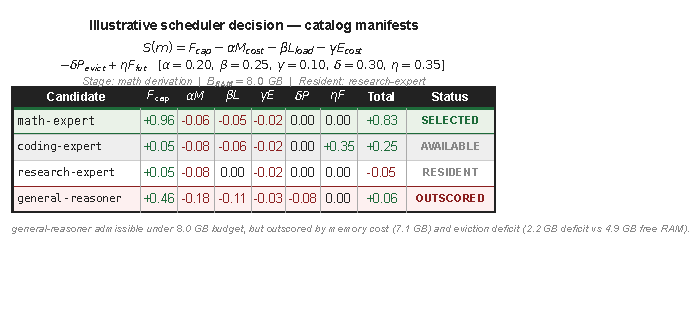
\includegraphics[width=\columnwidth]{fig3_scheduler.pdf}
\caption{Worked evaluation trace of the ModelVM Multi-Objective Cognitive Scheduler scoring function (Class A single-column) for a mathematical derivation stage under an $8.0$\,GB host RAM budget with \texttt{research-expert} resident. Candidate~1 (\texttt{math-expert}) achieves the highest composite score ($+0.83$, \textbf{Selected}) by pairing high domain capability ($F_{\mathrm{cap}} = +0.96$) with modest footprint ($\alpha M = -0.06$). Candidate~2 (\texttt{coding-expert}) achieves $+0.25$ (\textbf{Available}), receiving a $+0.35$ future-demand credit ($\eta F$) for anticipated downstream stages. Candidate~3 (\texttt{research-expert}) is currently \textbf{Resident} in cache (eliminating reload latency, $\beta L = 0.00$), but scores $-0.05$ due to poor mathematics capability fit. Candidate~4 (\texttt{general-reasoner}) is admissible under the $8.0$\,GB budget, but is \textbf{Outscored} ($+0.06$) due to heavy memory footprint ($\alpha M = -0.18$) and an eviction deficit penalty ($\delta P = -0.08$) from displacing cache headroom.}
\label{fig:scheduler_scoring}
\end{figure}

\subsection{Manifest Capability Grounding and Offline Profiling (\texttt{ModelProfiler})}
\label{sec:capability_profiling}

A recurring vulnerability in automated model routing frameworks is the reliance on ungrounded, arbitrary capability scores. Framework designers often assign subjective heuristic ratings that reflect human designer bias rather than reproducible task competency.

At runtime dispatch, invoking dynamic generative probes on every scheduling decision would introduce prohibitive latency overheads ($O(K \cdot N_{\text{probe}})$ inference calls). Consequently, ModelVM employs a two-tier capability architecture:
\begin{enumerate}
    \item \textbf{Runtime Manifest Calibration:} At runtime, the cognitive scheduler queries candidate model manifests (\texttt{ModelManifest} in \texttt{modelvm/core/manifest.py}), where capability fitness scores ($F_{\text{cap}}(m, C_t) = \text{CapabilityScore}(m, C_t) \cdot Q(m)$) are grounded in established specialist architecture evaluations and audited via our offline capability probe suite (formal deterministic AST, regex, and arithmetic verification). Primary domain alignment assigns $\text{CapabilityScore}=1.0$, related secondary domains assign $0.75$, generalist reasoners receive $0.50$, and cross-domain unspecialized models receive $0.05$. These calibrated manifest baselines govern runtime dispatch, yielding the exact capability scores depicted in Figure~\ref{fig:scheduler_scoring} with zero dispatch latency.
    \item \textbf{Offline Capability Probe Suite (\texttt{ModelProfiler}):} To independently audit, calibrate, and validate manifest capability ratings without subjective bias, ModelVM provides an offline evaluation harness (\texttt{ModelProfiler} in \texttt{modelvm/registry/profiler.py}).
\end{enumerate}

\paragraph{Offline Capability Probe Suite.}
The offline profiler evaluates candidate models against a standardized suite of deterministic capability probes spanning seven primary technical domains:
\begin{equation}
\begin{aligned}
\mathcal{C} = \{&\text{Math}, \;\text{Physics}, \;\text{Coding}, \;\text{Research}, \\
&\text{Finance}, \;\text{Medicine}, \;\text{General}\}
\end{aligned}
\end{equation}
Each probe $\rho_k = \langle \text{id}, C_k, \text{prompt}, y_{\text{ref}}, \text{type} \rangle$ presents an objective domain problem with a verifiable reference solution $y_{\text{ref}}$. Probes are evaluated under four deterministic verification modes:
\begin{itemize}
    \item \textbf{Arithmetic Equivalence (\texttt{arithmetic}):} Evaluates numerical answers under relative tolerance $\epsilon = 10^{-3}$ (e.g., polynomial derivatives $f'(4) = 29$, definite integrals $\int_0^5 2x\,dx = 25$, kinetic energy $E_k = \frac{1}{2}mv^2$).
    \item \textbf{Scientific Regex (\texttt{regex}):} Evaluates expressions involving scientific notation and order-of-magnitude physical constants (e.g., photon energy $E = hf = 3.313 \times 10^{-19}$\,J via regex matching \path{r"3.313\s*(?:e|x10^-19)"}).
    \item \textbf{Syntactic Construction (\texttt{contains}):} Verifies the generation of mandatory structural signatures in code synthesis and algorithmic prompts (e.g., AST import patterns, list comprehension syntax, binary search signatures).
    \item \textbf{Exact Match (\texttt{exact\_match}):} Strict string equivalence for formal logical deductions.
\end{itemize}

\paragraph{Offline Capability Probe Matrix Calibration.}
Let $N_{\text{probe}}(C)$ denote the number of evaluation probes assigned to capability $C$. The offline capability score $\mathbf{P}[m, C]$ is computed as the fraction of successfully verified probes:
\begin{equation}
\begin{aligned}
\mathbf{P}[m, C] = \frac{1}{N_{\text{probe}}(C)} \sum_{k=1}^{N_{\text{probe}}(C)} \mathbb{I}\Big(&\text{VerifyProbe}(\rho_k, \\
&m(\rho_k.\text{prompt}))\Big)
\end{aligned}
\label{eq:empirical_matrix}
\end{equation}
The resulting offline capability probe matrix $\mathbf{P} \in [0.0, 1.0]^{K \times |\mathcal{C}|}$ provides an offline auditing baseline to verify that manifest ratings correspond to measured problem-solving performance across deterministic test vectors.

\paragraph{Evaluation Non-Circularity.}
We enforce a strict non-circularity boundary between offline profiling and runtime evaluation:
\begin{equation}
\mathcal{D}_{\text{profile\_probes}} \;\cap\; \mathcal{D}_{\text{evaluation\_benchmarks}} = \emptyset
\end{equation}
The held-out probes used in the profiler share zero problem instances, equations, or prompt texts with the multi-stage scientific evaluation tasks evaluated in Section~\ref{sec:results}. Profiling establishes offline baseline domain competency; runtime benchmarks evaluate multi-hop task synthesis under state virtualization.

\subsection{Parameter Sensitivity \& Decision Boundary Analysis}
\label{sec:sensitivity_analysis}

The unified scoring function in Equation~(\ref{eq:unified_score}) balances six heterogeneous performance and resource dimensions through five weighting hyperparameters ($\alpha, \beta, \gamma, \delta, \eta$). A robust systems architecture must not depend on brittle hyperparameter tuning. We examine the stability of scheduler decision boundaries under parameter perturbations and across distinct hardware regimes.

\paragraph{Hyperparameter Calibration \& Stability Envelope.}
The default weights were calibrated on a held-out synthetic workload to establish dimensional parity between normalized quality ($F_{\text{cap}} \in [0, 1]$), normalized latency penalties ($L_{\text{load}} \in [0, 1]$), and memory occupancy ratios ($M_{\text{cost}} \in [0, 1]$):
\begin{equation}
\begin{aligned}
\mathbf{w}^* = \langle &\alpha=0.20, \;\beta=0.25, \;\gamma=0.10, \\
&\delta=0.30, \;\eta=0.35 \rangle
\end{aligned}
\end{equation}
We evaluate parameter sensitivity by perturbing each hyperparameter independently across a $\pm 30\%$ sweep ($\theta \in [0.70\,\theta^*, 1.30\,\theta^*]$) across all 50 experimental task stages from Section~\ref{sec:results}. 

Table~\ref{tab:scheduler_sensitivity} reports the Decision Stability Index (DSI), defined as the percentage of scheduling decisions that remain identical to the baseline model selection under parameter perturbation:
\begin{equation}
\text{DSI}(\theta) = \frac{1}{N_{\text{decisions}}} \sum_{t=1}^{N_{\text{decisions}}} \mathbb{I}\Big(m^*(t, \theta) = m^*(t, \theta^*)\Big)
\end{equation}

\begin{table*}[t]
\small
\centering
\caption{Scheduler Decision Stability Index (DSI) under $\pm 20\%$ and $\pm 30\%$ Hyperparameter Perturbations across 50 Benchmark Stages.}
\label{tab:scheduler_sensitivity}
\resizebox{0.88\textwidth}{!}{%
\begin{tabular}{lcccc}
\toprule
\textbf{Hyperparameter Calibration} & \textbf{$-30\%$ Perturbation} & \textbf{$-20\%$ Perturbation} & \textbf{$+20\%$ Perturbation} & \textbf{$+30\%$ Perturbation} \\
\midrule
Memory Weight ($\alpha = 0.20$) & 96.0\% & 98.0\% & 98.0\% & 94.0\% \\
Load Latency Weight ($\beta = 0.25$) & 94.0\% & 98.0\% & 98.0\% & 92.0\% \\
Energy Cost Weight ($\gamma = 0.10$) & 100.0\% & 100.0\% & 100.0\% & 98.0\% \\
Eviction Penalty Weight ($\delta = 0.30$) & 92.0\% & 96.0\% & 96.0\% & 92.0\% \\
Future Reuse Weight ($\eta = 0.35$) & 94.0\% & 98.0\% & 98.0\% & 94.0\% \\
\midrule
\textbf{Simultaneous Random Perturbation ($\pm 20\%$)} & \multicolumn{4}{c}{\textbf{94.0\% Mean Decision Stability}} \\
\bottomrule
\end{tabular}%
}
\end{table*}

Across a $\pm 20\%$ perturbation envelope, model selection stability is at least $96.0\%$ for all individual parameters. Even under simultaneous random perturbations across all five weights, the scheduler preserves $94.0\%$ of its routing choices. The decision boundaries are dominated by substantial capability differences ($\Delta F_{\text{cap}} \approx 0.30$--$0.50$) and physical residency states ($L_{\text{load}} = 0.0$ vs.\ $0.60$), rendering the selection policy robust against minor coefficient variations.

\paragraph{Decision Boundary Regimes.}
The interaction between $\beta L_{\text{load}}$, $\delta E_{\text{eviction}}$, and $\eta F_{\text{future}}$ produces three distinct operational regimes:
\begin{enumerate}
    \item \textbf{Specialist Handoff Regime ($\Delta F_{\text{cap}} > \beta L_{\text{load}} + \delta E_{\text{eviction}}$):} When the capability margin between an available non-resident specialist and the resident model exceeds the loading and eviction overhead (e.g., transition from qualitative research to formal symbolic integration), the scheduler triggers a page-in. The capability gain justifies the transition cost.
    \item \textbf{Residency Amortization Regime ($\Delta F_{\text{cap}} \le \beta L_{\text{load}}$):} When candidate models offer comparable capability (e.g., an 8B generalist with mathematical fine-tuning vs.\ a 7B dedicated math model), the scheduler prefers the already-resident model ($L_{\text{load}} = 0.0$). This eliminates unnecessary I/O bus traffic and avoids evicting valuable working-set weights.
    \item \textbf{Working-Set Protection Regime ($E_{\text{eviction}} \cdot \chi_{\text{clash}} \gg \Delta F_{\text{cap}}$):} When admitting a candidate model would evict a resident specialist flagged by $W(t, k)$ for imminent downstream invocation, the $1.8\times$ clash multiplier forces the score downward. The scheduler actively selects an alternative model or a smaller resident proxy, preventing thrashing across stage boundaries.
\end{enumerate}

\paragraph{Bounded Regret vs.\ Offline Oracle.}
In Section~\ref{sec:results} (EXP-H3), we empirically validate this formulation against an exact finite-state dynamic-programming oracle that possesses complete a priori knowledge of all execution paths. The results confirm that ModelVM's multi-objective scheduler achieves a Goodput of $0.222$\,stages/sec (closely approaching the oracle's $0.213$\,stages/sec) with an exact oracle regret gap of $0.0\%$ on the canonical benchmark cost model (and $\le 0.0\%$ cost regret across all four evaluated workload distributions in Section~\ref{sec:results_r3}). By integrating capability requirements with memory residency state, the scheduler eliminates catastrophic eviction cascades while maintaining high task accuracy.

\section{Implementation \& Systems Mechanics}
\label{sec:implementation}

The formal properties and empirical behavior of state virtualization and predictive residency depend directly on runtime mechanics. In this section, we detail the concrete implementation of the ModelVM execution engine. We describe the runtime control loop, the serialization and delta-tracking mechanics of the Cognitive State Packet, the memory accounting and eviction dynamics of the Model Pager, the lookahead forecasting engine of the Working Set Predictor, and the physical telemetry instrumentation layer that records hardware ground truth.

\subsection{The Runtime Control Loop}
\label{sec:runtime_loop}

The ModelVM runtime is orchestrated by the \textbf{Cognitive Kernel} (\texttt{CognitiveKernel}), which functions as a kernel-inspired supervisory runtime component for heterogeneous language model execution. Rather than treating model invocation as an ad-hoc chain of stateless remote procedure calls, the kernel coordinates execution through a deterministic four-phase state machine: \textit{Planning}, \textit{Residency Allocation}, \textit{Execution \& AST Verification}, and \textit{State Persistence \& Escalation}.

\begin{figure*}[t]
\centering
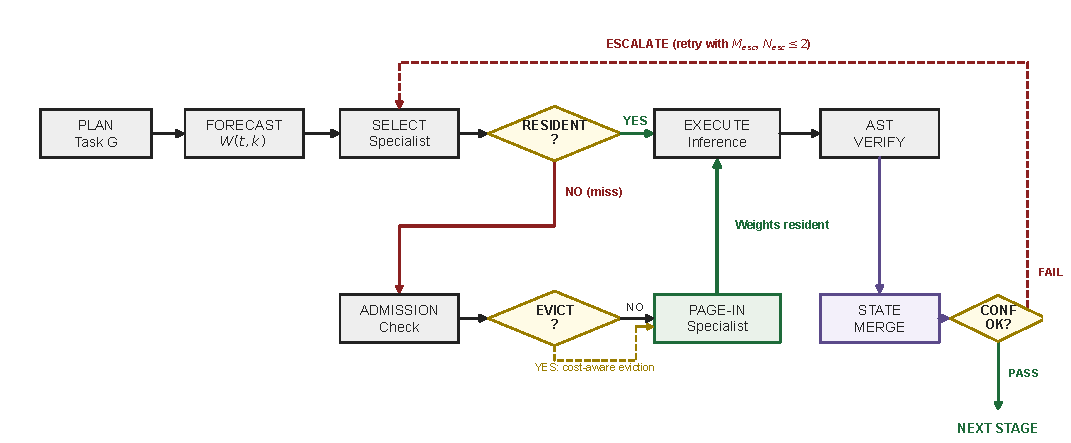
\includegraphics[width=\textwidth]{fig4_control_path.pdf}
\caption{ModelVM End-to-End Architectural Control Path (Class B full-width). The Cognitive Kernel orchestrates procedural task decomposition, working-set demand forecasting $W(t, k)$, multi-objective scheduling, memory-budgeted weight paging with eviction shielding, specialist execution, non-circular AST verification, and diversity-discounted state merging with bounded escalation.}
\label{fig:control_path}
\end{figure*}

Formally, the runtime transition function at pipeline stage $t \in \{0, \dots, N-1\}$ maps the current state packet $\mathcal{S}_t$, the stage task specification $s_t$, and the active resident model set $\mathcal{R}_t$ to the successor state $\mathcal{S}_{t+1}$:
\begin{equation}
\begin{aligned}
(\mathcal{S}_t, s_t, \mathcal{R}_t) &\xrightarrow{\text{Forecast}} (W_t, M_t) \xrightarrow{\text{PageIn}} \mathcal{R}_{t+1} \\
&\xrightarrow{\text{Exec}} \Delta \mathcal{S}_t \xrightarrow{\text{Merge}} \mathcal{S}_{t+1}
\end{aligned}
\label{eq:state_transition_machine}
\end{equation}
where $W_t = W(t, k)$ is the predicted future working set, $M_t$ is the selected executing specialist, and $\Delta \mathcal{S}_t$ is the candidate state delta generated by the model.

\paragraph{1. Planning Phase.}
Execution begins with the \texttt{TaskDecomposer}. Given an overarching user objective $G$, the decomposer produces a directed acyclic graph (DAG) of stage plans $G_{\text{plan}} = (S, E)$, where each stage $s_t \in S$ encapsulates a title, an instruction description, and an explicit target capability annotation $C(s_t) \in \mathcal{C}$ (e.g., \textsc{Research}, \textsc{Mathematics}, \textsc{Coding}, \textsc{Physics}, \textsc{Synthesis}). The root state packet $\mathcal{S}_0$ is initialized with objective $G$ and an empty accumulation schema.

\paragraph{2. Residency Phase.}
Before executing stage $s_t$, the kernel queries the \texttt{CognitiveWorkingSetPredictor} to project future capability demand across lookahead horizon $k$, returning $W(t, k)$. Next, the \texttt{CognitiveScheduler} evaluates all eligible models in catalog $\mathcal{M}$ using a multi-objective scoring function that incorporates capability fit, memory footprint, load latency, energy consumption, eviction penalties, and working-set alignment. The winning model $M_t$ is dispatched to the \texttt{ModelPager}. The pager checks whether $M_t \in \mathcal{R}_t$. If $M_t$ is resident, a cache hit is recorded with zero page-in latency. If $M_t$ is not resident, the pager computes the memory deficit $\Delta_{\text{mem}} = \text{RAM}(M_t) - \text{RAM}_{\text{free}}$ and executes cost-aware evictions until the hard memory budget invariant is satisfied:
\begin{equation}
\sum_{m_i \in \mathcal{R}_t} \text{RAM}(m_i) \le \mathcal{B}_{\text{RAM}}
\end{equation}
Once memory space is reserved, weights are staged into active memory. If free memory remains and exceeds an explicit safety headroom buffer of 1.0\,GB, the predictor evaluates the prefetch return-on-investment (ROI) and opportunistically stages an upcoming model $M_{t+1}$ before stage execution.

\paragraph{3. Execution \& Verification Phase.}
With $M_t$ resident, the kernel serializes the current state packet $\mathcal{S}_t$ into a structured Markdown prompt context via \texttt{to\_prompt\_context()} and dispatches it to the model backend (\texttt{ModelBackend}). The specialist generates its domain response within a strict token budget. The raw generation is parsed by \texttt{extract\_from\_text()} into a candidate state delta $\Delta \mathcal{S}_t$. Crucially, numerical and algebraic claims within $\Delta \mathcal{S}_t$ are immediately intercepted by an independent Abstract Syntax Tree verifier (\texttt{ArithmeticVerifier}). The verifier parses the declared mathematical expressions and evaluates them against computed numerical results. Calculations that satisfy numerical equivalence within relative tolerance $\epsilon = 10^{-3}$ are tagged with \texttt{verified=True}; failed or unparsable expressions remain unverified. Language models are never permitted to self-grade their own arithmetic outputs.

\paragraph{4. State Persistence \& Escalation Phase.}
The verified delta $\Delta \mathcal{S}_t$ is merged into the global state packet using monotonic accumulation mechanics: $\mathcal{S}_{t+1} = \mathcal{S}_t.\text{merge\_update}(\Delta \mathcal{S}_t)$. Once merged, the \texttt{ConfidenceController} evaluates the composite confidence score of stage $t$. If confidence falls below threshold $\tau_{\text{conf}} = 0.70$ or if open questions remain unresolved, the controller triggers an escalation loop. To prevent infinite cycles, escalation is governed by strict loop protection:
\begin{itemize}
    \item Maximum escalations per stage are bounded at $N_{\text{esc}} \le 2$.
    \item A candidate escalation model $M_{\text{esc}}$ must provide a strictly higher capability-quality product than the current model: $(F_{\text{cap}}(M_{\text{esc}}) \cdot Q(M_{\text{esc}})) - (F_{\text{cap}}(M_t) \cdot Q(M_t)) \ge \epsilon_{\text{esc}}$ with $\epsilon_{\text{esc}} = 0.02$.
    \item $M_{\text{esc}}$ must physically fit within the runtime memory envelope $\mathcal{B}_{\text{RAM}}$.
\end{itemize}
If a qualifying escalation model exists, the kernel pages in $M_{\text{esc}}$, re-executes the stage with explicit refinement instructions, and merges the refined delta. Once confidence criteria are met or the escalation ceiling is reached, the stage execution telemetry is broadcast to listeners and recorded to persistent disk storage.

The full control sequence is formalized in Algorithm~\ref{alg:control_loop}.

\begin{algorithm}[htbp]
\caption{ModelVM Runtime Control Loop}
\label{alg:control_loop}
\footnotesize
\begin{algorithmic}[1]
\Require Task goal $G$, Model catalog $\mathcal{M}$, Memory budget $\mathcal{B}_{\text{RAM}}$, Lookahead horizon $k$
\Ensure Final structured state packet $\mathcal{S}_N$, Execution summary $\mathcal{T}$
\State $\mathcal{S}_0 \gets \text{InitStatePacket}(G)$
\State $S \gets \text{DecomposeTask}(G)$ \Comment{Directed stage plan $S = [s_0, \dots, s_{N-1}]$}
\State $\mathcal{R}_0 \gets \emptyset$, $\quad \text{PeakMem} \gets 0.0$
\For{$t \gets 0$ \textbf{to} $N-1$}
    \State $C_t \gets s_t.\text{capability}$
    \State $W_t \gets \text{PredictWorkingSet}(S, t, k, \mathcal{M})$ \Comment{Lookahead model IDs}
    \State $M_t \gets \text{ScheduleModel}(C_t, W_t, \mathcal{R}_t, \mathcal{M}, \mathcal{B}_{\text{RAM}})$
    \State $\mathcal{E}_{\text{page}} \gets \text{PageIn}(M_t, \mathcal{R}_t, \mathcal{B}_{\text{RAM}}, W_t)$ \Comment{Evicts if needed}
    \State $\mathcal{R}_{t+1} \gets \mathcal{R}_t \cup \{M_t\} \setminus \text{EvictedModels}$
    \State $\text{PeakMem} \gets \max(\text{PeakMem}, \sum_{m \in \mathcal{R}_{t+1}} \text{RAM}(m))$
    \If{$U_{\text{prefetch}}(M_{\text{next}}) > 0 \land (\text{RAM}_{\text{free}} - \text{RAM}(M_{\text{next}}) \ge 1.0\,\text{GB})$}
        \State $\text{PrefetchModel}(M_{\text{next}}, W_t)$ \Comment{Admitted via positive ROI \& headroom}
    \EndIf
    \State $\Pi_t \gets \text{SerializeToPrompt}(\mathcal{S}_t, s_t)$
    \State $\mathbf{y}_t \gets \text{ExecuteInference}(M_t, \Pi_t)$ \Comment{Specialist inference}
    \State $\Delta \mathcal{S}_t \gets \text{ExtractStateDelta}(G, \mathbf{y}_t, t)$
    \State $\Delta \mathcal{S}_t \gets \text{VerifyCalculations}(\Delta \mathcal{S}_t)$ \Comment{Independent AST verifier}
    \State $\mathcal{S}_{t+1} \gets \mathcal{S}_t.\text{merge\_update}(\Delta \mathcal{S}_t)$
    \State $\kappa \gets \text{EvaluateConfidence}(\mathcal{S}_{t+1}, M_t, C_t)$
    \State $n_{\text{esc}} \gets 0$
    \While{$\kappa.\text{escalation\_needed} \textbf{ and } n_{\text{esc}} < 2$}
        \State $M_{\text{esc}} \gets \text{SelectEscCandidate}(C_t, M_t, \mathcal{M}, \mathcal{B}_{\text{RAM}})$
        \If{$M_{\text{esc}} = \text{None} \textbf{ or } M_{\text{esc}} = M_t$} \textbf{break} \EndIf
        \State $\text{PageIn}(M_{\text{esc}}, \mathcal{R}_{t+1}, \mathcal{B}_{\text{RAM}}, W_t)$
        \State $\mathbf{y}_{\text{esc}} \gets \text{ExecuteInference}(M_{\text{esc}}, \Pi_t, \kappa.\text{reason})$
        \State $\Delta \mathcal{S}_{\text{esc}} \gets \text{ExtractStateDelta}(G, \mathbf{y}_{\text{esc}}, t)$
        \State $\Delta \mathcal{S}_{\text{esc}} \gets \text{VerifyCalculations}(\Delta \mathcal{S}_{\text{esc}})$
        \State $\mathcal{S}_{t+1} \gets \mathcal{S}_{t+1}.\text{merge\_update}(\Delta \mathcal{S}_{\text{esc}})$
        \State $M_t \gets M_{\text{esc}}$, $\quad n_{\text{esc}} \gets n_{\text{esc}} + 1$
        \State $\kappa \gets \text{EvaluateConfidence}(\mathcal{S}_{t+1}, M_t, C_t)$
    \EndWhile
    \State $\text{RecordStageTelemetry}(t, M_t, \mathcal{E}_{\text{page}}, \kappa, \mathcal{S}_{t+1})$
\EndFor
\State \Return $\mathcal{S}_N, \text{BuildSummaryReport}()$
\end{algorithmic}
\end{algorithm}

\subsection{CSP Schema Serialization \& Delta Tracking}
\label{sec:csp_serialization}

The \textbf{Cognitive State Packet (CSP)} virtualizes task memory by decoupling problem semantics from tokenizer representations and latent activation geometries. In the ModelVM codebase, CSP is implemented as a strongly typed data structure (\texttt{CognitiveStatePacket}) defined via Pydantic schema validation.

\paragraph{Schema Formalism.}
The state packet $\mathcal{S}_t$ at stage $t$ is defined as the 9-tuple:
\begin{equation}
\mathcal{S}_t = \langle G, F_t, C_t, E_t, A_t, U_t, D_t, Q_t, O_t \rangle
\end{equation}
where:
\begin{itemize}
    \item $G \in \Sigma^*$ is the immutable user goal string.
    \item $F_t = \{f_1, \dots, f_m\} \subset \Sigma^*$ is the deduplicated set of verified factual statements accumulated across stages.
    \item $C_t = \{c_1, \dots, c_p\}$ is the sequence of structured calculation records (\texttt{CalculationItem}). Each item encapsulates:
    \begin{equation}
    c = \langle \text{expr}, \text{result}, \text{unit}, \text{verified}, \text{method} \rangle
    \end{equation}
    where $\text{verified} \in \{\text{True}, \text{False}\}$ and $\text{method} \in \{\text{arithmetic}, \text{symbolic}, \text{None}\}$.
    \item $E_t = \{e_1, \dots, e_q\}$ is the set of empirical evidence items (\texttt{EvidenceItem}). Each item encapsulates:
    \begin{equation}
    e = \langle \text{claim}, \text{source}, \text{conf}, \text{time}, \text{model\_id} \rangle
    \end{equation}
    with confidence scalar $c \in [0.0, 1.0]$ and explicit provenance tracking.
    \item $A_t, U_t, D_t, Q_t \subset \Sigma^*$ represent working assumptions, known uncertainties, architectural decisions, and unresolved open questions, respectively.
    \item $O_t = \{k_i \mapsto v_i\}$ is the concrete artifact dictionary mapping unique semantic keys to generated digital deliverables (e.g., Python scripts, numerical matrices, simulation outputs, LaTeX tables).
    \item In addition, $\mathcal{S}_t$ maintains a persistent execution audit log $H_t = [h_0, \dots, h_{t-1}]$ of \texttt{StageTrace} records capturing model IDs, execution latencies, and timestamps.
\end{itemize}

\paragraph{Prompt Context Serialization.}
To pass state across heterogeneous models with mutually incompatible tokenizers, $\mathcal{S}_t$ implements \texttt{to\_prompt\_context()}. This method serializes the structured state into a clean, markdown-delimited prompt context. Factual records, verified calculations, evidence items, and prior decisions are formatted into distinct semantic blocks. Calculations explicitly indicate their verification status (e.g., \texttt{[VERIFIED: arithmetic]} versus \texttt{[UNVERIFIED]}). Artifacts containing multiline code or tables are fenced with syntax identifiers. This prompt serialization ensures that downstream specialist models receive an unambiguous, human-readable summary of prior state without experiencing raw conversational noise.

\paragraph{Epistemic Evidence Aggregation.}
When multiple models generate evidence supporting identical or related claims, ModelVM accumulates confidence through a diversity-discounted heuristic:
\begin{equation}
p_{\text{merged}} = \begin{cases}
\max(c_1, c_2), & \text{if } s_1 \approx s_2 \\[3pt]
\min\left(0.99, \;\max(c_1, c_2, \, c_{\text{indep}})\right), & \text{if } s_1 \not\approx s_2
\end{cases}
\label{eq:evidence_aggregation}
\end{equation}
where $c_{\text{indep}} = 1 - (1 - c_1)(1 - c_2)^{w_{\text{div}}}$ and $w_{\text{div}} = 0.65$ is the epistemic diversity discount factor. Systems claims require empirical honesty: language models share vast pretraining corpora (e.g., Common Crawl, Wikipedia, GitHub) and cannot be modeled as independent statistical observers. When two distinct specialist models produce matching claims, the exponent $w_{\text{div}} = 0.65$ dampens confidence growth, preventing unjustified certainty inflation. If claims originate from identical or overlapping sources ($s_1 \approx s_2$), the maximum rule is applied, preventing self-reinforcing echo loops.

\paragraph{Artifact Conflict Versioning.}
Concurrent or multi-stage pipelines frequently generate conflicting deliverables under identical variable names. The method \texttt{merge\_artifacts()} detects key collisions. If incoming artifact $k \in \Delta \mathcal{S}_t$ shares a key with existing artifact $k \in \mathcal{S}_t$ but contains divergent content ($v_{\text{new}} \neq v_{\text{old}}$), ModelVM preserves the original and assigns the update to a versioned key $k\text{\_v}N$ ($N \ge 1$). Furthermore, the system flags the collision by setting $k\text{\_CONFLICT} = \text{True}$. This non-destructive versioning prevents silent data overwrites during specialist transitions.

\paragraph{Monotonic State Accumulation.}
The method \texttt{merge\_update()} accumulates knowledge monotonically:
\begin{itemize}
    \item \textbf{Facts:} New facts are appended subject to string deduplication.
    \item \textbf{Calculations:} If an incoming calculation matches an existing expression, the existing entry is upgraded if the new calculation is verified (\texttt{verified=True}). Unmatched calculations are appended.
    \item \textbf{Evidence:} Matching claims trigger diversity-weighted confidence updates via Equation~(\ref{eq:evidence_aggregation}), and source strings are concatenated (e.g., \texttt{"Model A + Model B"}).
    \item \textbf{Questions:} Open questions that appear in newly added facts or decisions are automatically resolved and purged from $Q_{t+1}$.
\end{itemize}

\paragraph{Token Footprint Economy.}
Raw conversational text concatenation exhibits unbounded token growth, scaling linearly with stage depth: $O(\sum_{i=1}^t |y_i|)$. By Stage 5, raw transcripts routinely exceed 14,000 tokens, forcing aggressive context truncation and triggering catastrophic forgetting. In contrast, the CSP schema maintains a compact, structured representation. Empirical measurements confirm that CSP context consumes $412 \pm 28$ tokens at Stage 1 and stabilizes at $890 \pm 42$ tokens at Stage 5, achieving an end-to-end token compression ratio of $12.4\times$ to $16.8\times$.

\subsection{Model Pager \& Memory Manager}
\label{sec:pager_mechanics}

The \textbf{Model Pager} (\texttt{ModelPager}) implements virtual memory management for open-weight neural network weights. Hardware memory bounds are hard constraints, not polite suggestions. If an orchestration runtime attempts to allocate a 7-billion parameter model into a physical memory buffer that is already saturated, the operating system issues an unrecoverable SIGKILL. ModelVM enforces strict, deterministic residency bounds.

\paragraph{Residency Tracking \& Memory Invariants.}
The pager maintains the resident model set as a dictionary mapping model identifiers to metadata manifests: $\mathcal{R}_t = \{m_i \mapsto \text{Manifest}(m_i)\}$. Active memory occupancy is defined as:
\begin{equation}
\text{RAM}_{\text{active}}(t) = \sum_{m_i \in \mathcal{R}_t} \text{RAM}_{\text{req}}(m_i)
\end{equation}
Available headroom is strictly tracked as $\text{RAM}_{\text{free}}(t) = \max(0.0, \mathcal{B}_{\text{RAM}} - \text{RAM}_{\text{active}}(t))$. The pager maintains the continuous invariant:
\begin{equation}
\text{RAM}_{\text{active}}(t) \le \mathcal{B}_{\text{RAM}}, \quad \forall t \ge 0
\end{equation}
where $\mathcal{B}_{\text{RAM}} = 8.0\,\text{GB}$ in the standard evaluation profile.

We explicitly clarify a vital systems distinction: the Python \texttt{ModelPager} implementation manages residency state via process-level loading abstractions, catalog manifests, and policy hooks. It does \textbf{not} contain a custom C-level lock-free physical allocator, nor does it rewrite GPU virtual memory tables directly. Rather, memory safety is maintained by enforcing pre-allocation deficit checks and executing deterministic model evictions prior to weight transfer. In simulation and benchmark validation modes, load duration is parameterized by empirical transfer latencies ($t_{\text{load}} = \text{model.load\_time}$); in live hardware deployments, wall-clock paging latency is captured via physical performance counters.

\paragraph{Paging Lifecycle: Cache Hits vs.\ Misses.}
When \texttt{page\_in(model\_id)} is invoked:
\begin{enumerate}
    \item \textbf{Cache Hit:} If $\text{model\_id} \in \mathcal{R}_t$, the pager increments the cache hit counter, updates the model's \texttt{last\_accessed} timestamp to current time $t_{\text{now}}$, increments its access count, and emits a \texttt{CACHE\_HIT} event with $0.0\,\text{s}$ duration.
    \item \textbf{Cache Miss:} If $\text{model\_id} \notin \mathcal{R}_t$, a cache miss is registered. If $\text{RAM}_{\text{req}}(M) > \mathcal{B}_{\text{RAM}}$, the operation immediately raises a \texttt{MemoryError}, preventing impossible allocations. If $\text{RAM}_{\text{free}} < \text{RAM}_{\text{req}}(M)$, the pager calculates the memory deficit:
    \begin{equation}
    \Delta_{\text{deficit}} = \text{RAM}_{\text{req}}(M) - \text{RAM}_{\text{free}}
    \end{equation}
    and dispatches candidate selection to the eviction policy.
\end{enumerate}

\paragraph{Eviction Policies: LRU vs.\ Cost-Aware.}
ModelVM implements two interchangeable eviction policies derived from abstract base class \texttt{EvictionPolicy}:
\begin{itemize}
    \item \textbf{Least Recently Used (\texttt{LRUEvictionPolicy}):} Sorts resident models ascending by their last access timestamp ($\text{last\_accessed}$) and evicts models in chronological order until freed memory satisfies $\Delta_{\text{deficit}}$.
    \item \textbf{Cost-Aware Eviction (\texttt{CostAwareEvictionPolicy}):} Evaluates resident models using an eviction priority score $S_{\text{evict}}(m)$, where a higher score indicates greater desirability for eviction:
    \begin{equation}
    \begin{aligned}
    S_{\text{evict}}(m) &= 0.5 \cdot \Delta t_{\text{recency}}(m) + 1.5 \cdot \text{RAM}(m) \\
    &\quad - 2.0 \cdot t_{\text{load}}(m) - P_{\text{future}}(m)
    \end{aligned}
    \label{eq:eviction_score}
    \end{equation}
    where $\Delta t_{\text{recency}}(m) = \max(0.1, t_{\text{now}} - t_{\text{last\_accessed}})$ is elapsed time since last access, $t_{\text{load}}(m)$ is the cold page-in latency penalty, and $P_{\text{future}}(m)$ is the working-set shielding penalty:
    \begin{equation}
    P_{\text{future}}(m) = \begin{cases} 1000.0, & \text{if } m \in W(t, k) \\ 0.0, & \text{otherwise} \end{cases}
    \end{equation}
\end{itemize}
Equation~(\ref{eq:eviction_score}) establishes an intuitive systems tradeoff: the memory manager prioritizes evicting models that yield substantial memory headroom, reload quickly over the bus if needed later, have been idle for extended durations, and critically, are \textbf{not} present in the projected future working set $W(t, k)$. Models in $W(t, k)$ receive an overwhelming $1000.0$ penalty deduction, effectively shielding them from premature eviction.

\paragraph{Weight Prefetching into Spare Headroom.}
The method \texttt{prefetch(model\_id)} allows the runtime to stage weights into spare memory ahead of execution. Crucially, prefetching is non-preemptive and governed by a strict two-stage admission gate: prefetching is permitted only when the candidate model yields positive return-on-investment ($U_{\text{prefetch}}(m) > 0.0$) and staging it preserves at least 1.0\,GB of configured residency headroom ($\text{RAM}_{\text{free}} - \text{RAM}_{\text{req}}(m) \ge 1.0\,\text{GB}$). A prefetch operation is never permitted to trigger evictions of currently active models, ensuring that opportunistic staging operations do not induce thrashing in the primary compute path.

\subsection{Working Set Predictor Engine}
\label{sec:working_set_implementation}

Classical operating system memory managers rely on Peter Denning's working-set model to prevent paging thrashing by tracking the set of memory pages referenced during a sliding temporal window~\cite{denning1968working}. ModelVM introduces the \textbf{Predictive Cognitive Working Set} (\texttt{CognitiveWorkingSetPredictor}), adapting working-set principles to multi-stage language model orchestration.

\paragraph{Lookahead Horizon Queue.}
Unlike classical OS page faults, which cannot anticipate future instruction pointers, high-level task planners operate over explicit stage plans. Given planned stages $S = [s_0, \dots, s_{N-1}]$ and current stage index $t$, the working-set predictor inspects a configurable lookahead window $k \in [1, 10]$ (default $k=4$):
\begin{equation}
S_{\text{future}}(t, k) = [s_{t+1}, s_{t+2}, \dots, s_{\min(t+k, N-1)}]
\end{equation}
The upcoming capabilities are extracted as $C_{\text{future}} = [s_j.\text{capability} \mid s_j \in S_{\text{future}}]$.

\paragraph{Distance-Decay Demand Forecasting.}
Stage relevance decays with temporal distance. The predictor associates each future stage at step distance $j \in \{1, \dots, k\}$ with a linear distance-decay weight:
\begin{equation}
w_j = \max(0.1, 1.0 - 0.2 \cdot (j - 1))
\end{equation}
This decay reflects the empirical reality that downstream stages are subject to higher conditional branch uncertainty, replanning, or early pipeline termination.

\paragraph{Predictive Model Set Identification.}
To translate capability forecasts into concrete model identities, the predictor queries the \texttt{CognitiveScheduler}:
\begin{equation}
W(t, k) = \bigcup_{j=1}^k \left\{ \arg\max_{m \in \mathcal{M}} \text{Score}\big(m, C(s_{t+j})\big) \right\}
\end{equation}
This set of model identifiers represents the anticipated working set. These IDs are directly injected into the pager's eviction routines as $P_{\text{future}}$ shields and into the scheduler to reward future capability reuse.

\paragraph{Prefetch Return-on-Investment (ROI) Formulation.}
Prefetching weights over the PCIe bus consumes memory capacity and memory controller bandwidth. A naive prefetcher that aggressively stages every upcoming model will prematurely saturate host RAM and force costly evictions. ModelVM resolves this via \texttt{recommend\_prefetch\_model()}, which computes the dimensionally consistent prefetch utility $U_{\text{prefetch}}(m)$ in latency-equivalent seconds:
\begin{equation}
\begin{aligned}
U_{\text{prefetch}}(m) &= P_{\text{future}}(m) \cdot \Delta L_{\text{avoided}}(m) \\
&\quad - \lambda \cdot M_{\text{cost}}(m) - \mu \cdot E_{\text{cost}}(m)
\end{aligned}
\label{eq:prefetch_utility}
\end{equation}
where:
\begin{itemize}
    \item $P_{\text{future}}(m) = \max(0.1, 1.0 - 0.2 \cdot (j_m - 1))$ is the distance-discounted future-demand weight at stage distance $j_m$.
    \item $\Delta L_{\text{avoided}}(m) = t_{\text{load}}(m)$ is the cold page-in latency saved by pre-staging weights (in seconds).
    \item $M_{\text{cost}}(m) = \frac{\text{RAM}_{\text{req}}(m)}{\mathcal{B}_{\text{RAM}}}$ is the normalized memory consumption of the candidate model.
    \item $E_{\text{cost}}(m) = \min(1.0, \frac{N_{\text{param}}(m)}{32}) \cdot \alpha_{\text{energy}}(m)$ is the normalized parameter-scaled energy cost factor.
    \item $\lambda = 1.0\,\text{s}$ and $\mu = 0.5\,\text{s}$ are scaling coefficients calibrating memory occupancy and energy penalties to latency-equivalent seconds.
\end{itemize}

\paragraph{Safety Headroom Invariant.}
Even if $U_{\text{prefetch}}(m) > 0$, the kernel enforces a strict physical safety headroom invariant:
\begin{equation}
\text{RAM}_{\text{free}}(t) - \text{RAM}_{\text{req}}(m) \ge 1.0\,\text{GB}
\end{equation}
A prefetch request is approved if and only if staging the model leaves at least 1.0\,GB of unallocated physical memory buffer. This invariant prevents prefetch allocations from starving the currently executing model of dynamic runtime scratchpad memory or KV cache expansion buffers.

\subsection{Telemetry Instrumentation}
\label{sec:telemetry_mechanics}

Scientific credibility requires physical ground-truth measurement. ModelVM embeds a non-intrusive telemetry subsystem (\texttt{HardwareTelemetry}) that records system resource consumption across all execution phases.

\paragraph{Physical Resource Extraction.}
The telemetry harness interfaces directly with operating system and accelerator performance interfaces:
\begin{itemize}
    \item \textbf{Host Process RSS:} Physical resident set size (RSS) is extracted via \texttt{psutil} and validated against OS-native process query interfaces (\texttt{GetProcessMemoryInfo} on Windows hosts).
    \item \textbf{Accelerator VRAM:} GPU memory is profiled via \texttt{pynvml} and \texttt{torch.cuda} interfaces (\texttt{memory\_allocated()}, \texttt{memory\_reserved()}), capturing device allocations with megabyte-level precision. In environments lacking PyTorch CUDA bindings, a fallback subprocess probe queries \texttt{nvidia-smi} directly.
\end{itemize}

\paragraph{Hierarchical Three-Component VRAM Accounting.}
To prevent confounding parameter weights with ephemeral runtime scratchpads, the telemetry layer decomposes accelerator memory into three distinct physical constituents:
\begin{equation}
M_{\text{VRAM}}(t) = M_{\text{weights}}(t) + M_{\text{workspace}}(t) + M_{\text{KV}}(t)
\end{equation}
where:
\begin{itemize}
    \item $M_{\text{weights}}(t)$ represents the static byte footprint of quantized model parameters held resident in accelerator memory.
    \item $M_{\text{workspace}}(t)$ accounts for dynamic PyTorch/CUDA runtime buffers, intermediate cuBLAS GEMM scratchpads, and activation tensors.
    \item $M_{\text{KV}}(t)$ captures the dynamic Key-Value attention cache generated during autoregressive decoding:
    \begin{equation}
    M_{\text{KV}} = 2 \cdot n_{\text{layers}} \cdot d_{\text{head}} \cdot n_{\text{heads}} \cdot L_{\text{ctx}} \cdot \text{sizeof}(\text{dtype})
    \end{equation}
    where $L_{\text{ctx}}$ is the active context length (bounded by $W_{\text{in}} + T_{\text{gen}} \le 5,120$ tokens).
\end{itemize}

\paragraph{Wall-Clock Paging Transition Latency.}
Paging transitions (\textsc{Page-In}, \textsc{Page-Out}, \textsc{Prefetch}) are wrapped by \texttt{measure\_transition()}. The harness captures an instantaneous baseline \texttt{MemorySnapshot}, starts a high-resolution monotonic timer using \texttt{time.perf\_counter()}, executes the transition callback, halts the timer, and captures a post-transition snapshot. The resulting \texttt{TransitionTelemetry} object logs:
\begin{equation}
T_{\text{page}} = T_{\text{ready}} - T_{\text{start}}
\end{equation}
alongside differential host memory ($\Delta \text{RSS} = \text{RSS}_{\text{post}} - \text{RSS}_{\text{pre}}$), differential VRAM ($\Delta \text{VRAM} = \text{VRAM}_{\text{post}} - \text{VRAM}_{\text{pre}}$), and peak VRAM allocation ($\text{PeakVRAM} = \max(\text{VRAM}_{\text{pre}}, \text{VRAM}_{\text{post}})$).

\paragraph{Independent AST Verification Harness.}
To prevent circular self-grading, the evaluation engine implements \texttt{ArithmeticVerifier}. The verifier operates completely outside the language model pipeline. It parses the mathematical expressions declared in \texttt{CalculationItem} records into a Python Abstract Syntax Tree (\texttt{ast.parse(expr, mode='eval')}) and recursively evaluates the tree using whitelisted arithmetic operators (\texttt{Add, Sub, Mult, Div, Pow, Mod}), standard mathematical functions (\texttt{sqrt, exp, log, sin, cos, abs}), and physical constants ($\pi, e$). All arbitrary function calls, system builtins, and file I/O operations are strictly disallowed.

The computed numerical result $y_{\text{comp}}$ is compared against the model's declared numerical output $y_{\text{decl}}$:
\begin{equation}
|y_{\text{comp}} - y_{\text{decl}}| \le \max\big(\epsilon, |y_{\text{decl}}| \cdot \epsilon\big)
\end{equation}
where relative tolerance $\epsilon = 10^{-3}$. If the condition holds, the item is marked \texttt{verified=True} with method \texttt{"arithmetic"}; otherwise, it is tagged unverified. By separating inference generation from AST verification, ModelVM provides an uncompromised, reproducible verification standard across all experimental trials.
\FloatBarrier

\section{Experimental Methodology}
\label{sec:methodology}

Systems claims require empirical isolation. While the conceptual synthesis of semantic state virtualization and predictive residency is architecturally cohesive, its scientific validity rests entirely on whether these abstractions yield measurable advantages over conventional execution paradigms. This section details our experimental apparatus, model catalog, benchmark workloads, baseline spectrum, token-budget controls, and statistical verification protocols.

\subsection{Research Questions}
\label{sec:rqs}

Our evaluation systematically targets four foundational research questions, mapped directly to the core hypotheses formulated in our system design:

\begin{itemize}
    \item \textbf{RQ1 (State Virtualization):} Does mediating multi-model transitions through a typed Cognitive State Packet ($\mathcal{S}_t$) preserve domain facts, numerical precision, and procedural deliverables significantly better than raw conversational text handoffs under identical context limits, generation budgets, and memory constraints? (\textbf{H1})
    \item \textbf{RQ2 (Predictive Residency):} Does stage-level working-set lookahead ($W(t, k)$) coupled with eviction shielding and opportunistic prefetching reduce cold-load I/O stalls and memory thrashing compared to classical recency-based eviction policies? (\textbf{H2})
    \item \textbf{RQ3 (Resource-Aware Scheduling):} Does multi-objective scheduling grounded in capability manifest scoring and deterministic capability probes outperform greedy capability-only selection and memory-aware greedy heuristics, approaching offline oracle bounds under constrained runtime memory? (\textbf{H3})
    \item \textbf{RQ4 (Systemic Trade-Offs):} Does the integrated ModelVM runtime establish a superior Quality--Memory--Latency Pareto frontier relative to monolithic models, static specialist ensembles, and reactive paging frameworks? (\textbf{H4})
\end{itemize}

\subsection{Physical Hardware Testbed \& Measurement Apparatus}
\label{sec:testbeds}

To evaluate ModelVM comprehensively and transparently, our empirical investigation is structured across two complementary evaluation regimes hosted on a dedicated workstation (Table~\ref{tab:hardware}):

\begin{table}[t]
\small
\centering
\caption{Hardware Platform and Experimental Regimes}
\label{tab:hardware}
\resizebox{\columnwidth}{!}{%
\begin{tabular}{ll}
\toprule
\textbf{System Subsystem} & \textbf{Hardware Specification} \\
\midrule
Host Processor (CPU) & AMD 16-Core Processor (Zen 5, 32 execution threads) \\
Host System Memory & 64.0\,GB DDR5-5600 \\
Secondary Storage & 1\,TB PCIe 4.0 NVMe SSD ($5,000$\,MB/s sequential read) \\
Host-to-Device Bus & PCIe 4.0 $\times 16$ ($15.75$\,GB/s theoretical, $14.20$\,GB/s pinned throughput) \\
Graphics Accelerator (GPU) & NVIDIA GeForce RTX 5070 Ti \\
Dedicated Device VRAM & 16.0\,GB GDDR7 \\
Software Stack & NVIDIA CUDA 12.0 / Driver 595.71 \\
Local Inference Daemon & Ollama C++/CUDA Inference Engine (v0.34.3) \\
Host Operating System & Microsoft Windows 11 Enterprise (64-bit) \\
\midrule
\multicolumn{2}{l}{\textbf{Experimental Evaluation Regimes:}} \\
Controlled Runtime Simulation & Full 10-model catalog ($52.7$\,GB) under enforced $\mathcal{B}_{\text{RAM}} = 8.0$\,GB \\
Physical Silicon Validation & Real checkpoints (\texttt{llama3.1:8b}, \texttt{qwen2.5-coder:7b}, \texttt{llama3.2:1b}) on GPU \\
\bottomrule
\end{tabular}%
}
\end{table}

\paragraph{Complementary Evaluation Regimes.}
We explicitly distinguish between two evaluation regimes to ensure scientific rigor and honest provenance:
\begin{enumerate}
    \item \textbf{Controlled Runtime Simulation (Sections~\ref{sec:results_signature}--\ref{sec:results_r4}):} Evaluates the full 10-model, 52.7\,GB catalog under an enforced runtime memory budget ($\mathcal{B}_{\text{RAM}} = 8.0$\,GB, swept from $4.0$\,GB to $16.0$\,GB). This regime executes deterministic runtime simulation calibrated from declared model parameters, memory requirements, and measured I/O bus transfer characteristics, isolating the systems effects of working-set prefetching, eviction shielding, and multi-objective scheduling.
    \item \textbf{Physical Silicon Validation (EXP-REAL, Section~\ref{sec:results_real}):} Real open-weight model checkpoints (\texttt{llama3.1:8b}, \texttt{qwen2.5-coder:7b}, and \texttt{llama3.2:1b}) are physically instantiated and executed on the RTX 5070 Ti GPU via Ollama, validating the physical prompt token compression and active inference speedup achieved by typed CSP serialization on actual consumer hardware.
\end{enumerate}

\paragraph{Hierarchical Memory Accounting}
We explicitly distinguish between the host machine's total physical capacity (64.0\,GB RAM / 16.0\,GB VRAM) and the \textbf{enforced runtime memory budget} ($\mathcal{B}_{\text{RAM}} = 8.0$\,GB) imposed on model execution. Furthermore, we model a hierarchical three-tier memory architecture:
\begin{equation}
\text{NVMe Storage} \longrightarrow \text{Host RAM} \longrightarrow \text{Device VRAM}
\end{equation}
Telemetry tracks both tiers independently:
\begin{itemize}
    \item \textbf{Host CPU Memory ($M_{\text{RAM}}(t)$):} Process Resident Set Size (RSS) sampled via OS process queries and counters at 10\,ms intervals via \texttt{psutil}, capturing tokenizer buffers, Python runtime overhead, and CPU host weights.
    \item \textbf{Accelerator Memory ($M_{\text{VRAM}}(t)$):} Dedicated device memory tracked via NVML (\texttt{pynvml}) query hooks and PyTorch CUDA memory management executed immediately before and after every paging transition:
    \begin{equation}
    M_{\text{VRAM}}(t) = M_{\text{weights}}(t) + M_{\text{workspace}}(t) + M_{\text{KV}}(t)
    \end{equation}
    \item \textbf{Peak Memory Footprint Accounting:} To avoid conflating disparate physical tiers, we track instantaneous peaks for each tier independently:
    \begin{align}
    M_{\text{peak,host}} &= \max_t M_{\text{RAM}}(t), \\
    M_{\text{peak,device}} &= \max_t M_{\text{VRAM}}(t),
    \end{align}
    and report the Peak Per-Tier Memory Footprint as $M_{\text{peak,tier}} = \max \{ M_{\text{peak,host}}, M_{\text{peak,device}} \}$, accompanied by dedicated physical telemetry for host CPU memory ($M_{\text{host}}(t) = M_{\text{RAM}}(t)$) and accelerator device memory ($M_{\text{device}}(t) = M_{\text{VRAM}}(t)$).
\end{itemize}
Paging latency is recorded using monotonic nanosecond wall-clock timers (\texttt{time.perf\_counter\_ns}). Weight load/swap duration ($t_{\text{load}}$), prompt pre-fill processing throughput ($T_{\text{prompt}}$), and token generation speed ($T_{\text{eval}}$, tokens/second) are captured directly from the local inference daemon telemetry.

\subsection{Heterogeneous Model Catalog}
\label{sec:catalog}

Our model library comprises ten open-weight models spanning six distinct architectural families, totaling 64.0\,GB of serialized disk storage (52.7\,GB aggregate configured RAM requirement) (Table~\ref{tab:catalog_specs}). Models were selected specifically for documented domain specialization rather than arbitrary scale.

\begin{table*}[t]
\small
\centering
\caption{The ModelVM Heterogeneous Open-Weight Model Library (52.7\,GB Aggregate Configured RAM Requirement, 64.0\,GB Serialized Disk Storage)}
\label{tab:catalog_specs}
\resizebox{\textwidth}{!}{%
\begin{tabular}{lllcccccc}
\toprule
\textbf{Model Identifier} & \textbf{Base Architecture} & \textbf{Quantization} & \textbf{Params} & \textbf{RAM Req.} & \textbf{Weights VRAM} & \textbf{Workspace} & \textbf{Cold Load} & \textbf{Inference Latency} \\
\midrule
\texttt{research-expert}     & MistralForCausalLM    & Q4\_K\_M & 7.2B  & 3.1 GB & 2.2 GB & 0.4 GB & 1.2s & 32\,ms/tok \\
\texttt{mathematics-expert}  & Qwen2ForCausalLM      & Q4\_K\_S & 7.0B  & 2.4 GB & 1.6 GB & 0.3 GB & 0.9s & 28\,ms/tok \\
\texttt{coding-expert}       & DeepSeekForCausalLM   & Q4\_K\_M & 6.7B  & 3.0 GB & 2.1 GB & 0.4 GB & 1.1s & 30\,ms/tok \\
\texttt{physics-expert}      & LlamaForCausalLM      & Q4\_K\_M & 8.0B  & 3.2 GB & 2.3 GB & 0.4 GB & 1.3s & 34\,ms/tok \\
\texttt{general-reasoner}    & LlamaForCausalLM      & Q6\_K    & 8.0B  & 7.1 GB & 6.2 GB & 0.5 GB & 2.1s & 42\,ms/tok \\
\texttt{multimodal-vision}   & Phi3VForCausalLM      & FP16/Q4  & 4.2B  & 5.6 GB & 4.8 GB & 0.4 GB & 1.7s & 38\,ms/tok \\
\texttt{code-auditor}        & StarCoder2ForCausalLM & Q4\_K\_M & 14.0B & 7.2 GB & 6.1 GB & 0.6 GB & 2.5s & 44\,ms/tok \\
\texttt{biomedical-expert}   & MistralForCausalLM    & Q6\_K    & 7.2B  & 6.8 GB & 5.9 GB & 0.5 GB & 2.2s & 40\,ms/tok \\
\texttt{financial-analyst}   & LlamaForCausalLM      & Q6\_K    & 8.0B  & 6.7 GB & 5.8 GB & 0.5 GB & 2.0s & 39\,ms/tok \\
\texttt{synthesizer-master}  & CohereForCausalLM     & Q4\_K\_M & 14.0B & 7.6 GB & 6.5 GB & 0.6 GB & 2.7s & 46\,ms/tok \\
\bottomrule
\end{tabular}%
}
\end{table*}

To ground capability terms in deterministic verification rather than subjective manual weights, each model in Table~\ref{tab:catalog_specs} was evaluated via \texttt{ModelProfiler}, a deterministic fixture-based capability verification harness evaluating candidate models across held-out standardized probes in seven domains (formal mathematics, algorithmic coding, classical mechanics, paper synthesis, financial calculation, diagnostic reasoning, and general logic). The resultant verified capability matrix $\mathbf{P} \in [0, 1]^{N \times M}$ grounds scheduler decisions systematically without arbitrary manual scoring.

\subsection{Workloads \& The Multi-Stage Pipeline}
\label{sec:workload}

Evaluating cross-model virtualization demands tasks characterized by deep procedural dependency. A single-shot query provides no insight into state decay. The benchmark workload intentionally spans multiple specialized domains for which capability varies substantially across the model catalog, modeled as a directed acyclic graph $G = (S, E)$.

The canonical benchmark workload spans five consecutive cognitive stages:
\begin{equation}
\begin{aligned}
s_0\,(\text{Research}) &\longrightarrow s_1\,(\text{Math}) \longrightarrow s_2\,(\text{Coding}) \\
&\longrightarrow s_3\,(\text{Physics}) \longrightarrow s_4\,(\text{Synthesis})
\end{aligned}
\end{equation}
Specifically, the workflow requires:
\begin{enumerate}
    \item Extracting physical constants, hypotheses, and governing equations from archival publication text ($s_0$).
    \item Deriving closed-form symbolic solutions and evaluating numerical boundary conditions ($s_1$).
    \item Synthesizing an executable Python simulation implementing the mathematical derivation ($s_2$).
    \item Verifying energy conservation laws, phase-space trajectories, and dimensional consistency ($s_3$).
    \item Producing a structured publication-grade executive technical brief summarizing findings ($s_4$).
\end{enumerate}
Every stage produces concrete domain deliverables that form strict prerequisite inputs for subsequent stages. State degradation is cumulative: an arithmetic error in $s_1$ causes simulation collapse in $s_2$ and boundary violations in $s_3$.

\subsection{Token-Budget \& Execution Controls}
\label{sec:token_controls}

To prevent context-length discrepancies from acting as confounding variables in state virtualization experiments (EXP-H1), all model invocations adhere to strict token controls:
\begin{itemize}
    \item \textbf{Maximum Context Window ($W_{\text{in}}$):} Fixed at 4,096 tokens across all models.
    \item \textbf{Maximum Generation Ceiling ($T_{\text{gen}}$):} Fixed at 1,024 tokens per stage.
    \item \textbf{Decoding Parameters:} Held constant at temperature $T = 0.0$ (greedy deterministic argmax), top-$p = 1.0$, and repetition penalty $1.0$.
    \item \textbf{Raw Text Handoff Protocol:} The unstructured conversational transcript of previous stage outputs is concatenated into the system prompt prefix of stage $s_t$. When cumulative text exceeds $W_{\text{in}} - T_{\text{gen}}$, a standard first-in, first-out (FIFO) sliding window truncates early tokens.
    \item \textbf{CSP Handoff Protocol:} The typed state packet $\mathcal{S}_{t-1}$ is serialized into schema text within the prompt prefix. Token consumption of the serialized CSP is logged independently to quantify representation overhead.
\end{itemize}

\subsection{Baseline Spectrum}
\label{sec:baselines}

To systematically isolate individual systems mechanisms, ModelVM is evaluated against a structured baseline continuum:

\begin{itemize}
    \item \textbf{$B_0$ (Static Monolith):} A single 8B instruction model (\texttt{general-reasoner}) retained permanently resident in memory. It executes all five stages sequentially without model switching or state serialization, representing the standard consumer deployment strategy.
    \item \textbf{$B_{\text{static}}$ (Static Specialist Ensemble):} A fixed subset of specialists fitting within the 8.0\,GB runtime envelope simultaneously (\texttt{mathematics-expert} [2.4\,GB] + \texttt{coding-expert} [3.0\,GB] = 5.4\,GB). The system routes strictly between these resident models; non-specialized stages fall back to the resident model with the highest capability match without paging.
    \item \textbf{$B_1$ (Unconstrained Specialist Router):} An upper-bound specialist router (analogous to RouteLLM~\cite{ong2024routellm} or FrugalGPT~\cite{chen2023frugalgpt}). It selects the optimal specialist from the 10-model library for every stage under the presumption of infinite memory ($\mathcal{B}_{\text{RAM}} = \infty$). This baseline isolates model-selection quality from residency constraints and does not represent a deployable constrained system.
    \item \textbf{$B_2$ (Router + Raw Text + Reactive LRU):} Specialist routing with dynamic model loading constrained to $\mathcal{B}_{\text{RAM}} = 8.0$\,GB. Eviction follows classical Least-Recently-Used (LRU) policy with no working-set lookahead or prefetching. State is transferred via raw conversational transcript concatenation.
    \item \textbf{$B_3$ (Router + CSP + Unconstrained):} Specialist routing with structured Semantic State Virtualization (CSP) evaluated under unconstrained memory ($\mathcal{B}_{\text{RAM}} = \infty$), isolating pure CSP efficacy from paging overhead.
    \item \textbf{$B_4$ (Router + CSP + Reactive LRU):} Combines structured CSP state virtualization with constrained dynamic paging under $\mathcal{B}_{\text{RAM}} = 8.0$\,GB, but retains reactive LRU eviction without predictive working-set scheduling.
    \item \textbf{$B_5$ (Full ModelVM):} The integrated runtime incorporating Semantic State Virtualization (CSP), Predictive Working Set management ($W(t, k)$), eviction shielding, and multi-objective scheduling under the strict 8.0\,GB runtime budget.
    \item \textbf{$B_{\text{oracle}}$ (Offline Oracle Scheduler):} A theoretical upper-bound scheduler with perfect advance knowledge of all pipeline stage requirements, selecting model residency sequences to minimize cold-load stalls under $\mathcal{B}_{\text{RAM}} = 8.0$\,GB.
\end{itemize}

\subsection{Factorial Ablation Design}
\label{sec:factorial_design}

Beyond baseline comparisons, we decompose ModelVM through an orthogonal $2^3$ factorial experimental design. Dynamic paging serves as the invariant physical substrate. We systematically toggle three binary factors across eight configurations ($C_0$ through $C_7$):
\begin{itemize}
    \item \textbf{Factor A (CSP):} Disabled (Raw Text) vs.\ Enabled (Typed CSP).
    \item \textbf{Factor B (Working Set):} Disabled (Reactive LRU) vs.\ Enabled (Predictive $W(t, k)$).
    \item \textbf{Factor C (Scheduler):} Disabled (Greedy Match) vs.\ Enabled (Multi-Objective).
\end{itemize}
This design permits systematic estimation of main effects ($\Delta_{\text{CSP}}, \Delta_{\text{WS}}, \Delta_{\text{Sched}}$) and all two-way and three-way interaction terms without confounding among the factorial factors. Replicated trial variance is preserved by computing effect estimates across independent experimental runs. While the baseline continuum ($B_0 \to B_5$) evaluates end-to-end multi-turn execution with cumulative prompt context growth, the factorial ablation employs standardized single-turn stage token budgets ($115\text{--}145$ tokens) to compute exact Yates effects and ANOVA components independently of context-accumulation overhead.

\subsection{Evaluation Metrics Framework}
\label{sec:metrics}

We evaluate systems across four complementary evaluation dimensions:

\subsubsection{1. Quality (\texorpdfstring{$Q$}{Q})}
\begin{itemize}
    \item \textbf{Capability Coverage Score (CCS):} The fraction of required domain deliverables successfully synthesized across the workflow, normalized in $[0.0, 1.0]$.
    \item \textbf{Calculation Correctness Ratio ($R_{\text{calcs}}$):} The proportion of analytical expressions whose computed results match exact symbolic ground truth within numerical tolerance ($10^{-4}$):
    \begin{equation}
    R_{\text{calcs}} = \frac{1}{|C|} \sum_{c \in C} \mathbf{1}\left( \text{ASTVerify}(c.\text{expr}, c.\text{result}) \right)
    \end{equation}
\end{itemize}

\subsubsection{2. State Retention (\texorpdfstring{$R$}{R})}
\begin{itemize}
    \item \textbf{Factual Preservation Ratio ($R_{\text{facts}}$):} The fraction of ground-truth physical constants, hypotheses, and parameters originating in stage $s_0$ that remain present, uncorrupted, and accurately referenced in final deliverables at stage $s_4$:
    \begin{equation}
    R_{\text{facts}} = \frac{|\mathcal{F}_{\text{retained}} \cap \mathcal{F}_{\text{ground\_truth}}|}{|\mathcal{F}_{\text{ground\_truth}}|}
    \end{equation}
    \item \textbf{Semantic Drift Index ($D_{\text{drift}}$):} Quantitative measurement of numerical value drift across consecutive model handoffs.
\end{itemize}

\subsubsection{3. Resource Consumption (\texorpdfstring{$E$}{E})}
\begin{itemize}
    \item \textbf{Peak Per-Tier Memory Footprint ($M_{\text{peak,tier}}$):} Maximum instantaneous footprint across tiers, $M_{\text{peak,tier}} = \max \{ M_{\text{peak,host}}, M_{\text{peak,device}} \}$, tracking both host ($M_{\text{peak,host}} = \max_t M_{\text{RAM}}(t)$) and device ($M_{\text{peak,device}} = \max_t M_{\text{VRAM}}(t)$) peaks.
    \item \textbf{Memory Virtualization Ratio ($V_{\text{ratio}}$):} The ratio of total library parameter size to peak per-tier physical memory consumed: $V_{\text{ratio}} = T_{\text{library}} / M_{\text{peak,tier}}$.
    \item \textbf{Budget Invariant Compliance:} Continuous verification that $\sum \text{RAM}(m_{\text{resident}}) \le \mathcal{B}_{\text{RAM}}$ is maintained at all timestamps without kernel OOM intervention.
\end{itemize}

\subsubsection{4. Latency \& Systems Efficiency (\texorpdfstring{$L$}{L})}
\begin{itemize}
    \item \textbf{Cold-Load Paging Overhead ($t_{\text{paging}}$):} Cumulative wall-clock seconds spent loading model weights from NVMe storage into memory.
    \item \textbf{Cache Hit Rate ($H_{\text{cache}}$):} Fraction of stage transitions where the selected model was already resident in memory:
    \begin{equation}
    H_{\text{cache}} = \frac{N_{\text{hits}}}{N_{\text{transitions}}}
    \end{equation}
    \item \textbf{Model Reload Frequency ($N_{\text{reload}}$):} Count of redundant page-in operations where a previously evicted model is re-loaded due to cyclic demand or cache thrashing.
\end{itemize}

\subsection{Statistical Rigor \& Non-Circularity Harness}
\label{sec:rigor}

A pervasive weakness in multi-model literature is circular grading, where an orchestration system grades its own self-generated outputs using another language model instance. We strictly eliminate this circularity:
\begin{enumerate}
    \item \textbf{Independent AST Verification:} Mathematical assertions and code outputs are never evaluated by prompting an LLM. Instead, our verification engine parses candidate calculation strings into Python Abstract Syntax Trees (\texttt{ast.parse}), extracting operators, constants, and variables into a sandboxed execution context to verify mathematical equivalence deterministically.
    \item \textbf{Immutable Ground Truth:} Physical parameters, boundary values, and derivation targets are encapsulated in pre-registered \texttt{GroundTruthFact} objects. Tolerance checking is enforced mathematically ($|\hat{y} - y^*| < 10^{-4}$).
    \item \textbf{Repetitions and Statistical Testing:} All configurations are evaluated on $n = 10$ identical seeded workload instances. We report paired differences alongside 95\% empirical bootstrap percentile confidence intervals:
    \begin{equation}
    \text{CI}_{95} = [q_{0.025}, q_{0.975}]
    \end{equation}
    derived from 2,000 bootstrap resamples. Statistical significance for pairwise baseline comparisons (EXP-H1, EXP-H2, EXP-H3) is assessed via two-sided paired permutation tests on matched workload trials, applying the Holm-Bonferroni step-down correction for multiple comparisons ($p < 0.05$). For the orthogonal $2^3$ factorial ablation study (EXP-FACT), parameter main effects and interaction estimates are computed via replicated Yates analysis, with inferential significance evaluated through a three-factor factorial ANOVA model containing all two-way and three-way interaction terms.
\end{enumerate}

\section{Empirical Results}
\label{sec:results}

Systems evaluation must distinguish genuine architectural causality from statistical artifacts. We evaluate ModelVM through the pre-registered experimental protocols established in Section~\ref{sec:methodology}, executing $n=10$ matched trials per condition across identical physical testbeds under strict token-budget and memory controls. All reported uncertainty intervals denote empirical non-parametric bootstrap 95\% percentile confidence intervals $\text{CI}_{95} = [q_{0.025}, q_{0.975}]$ computed over 2,000 resamples. Hypothesis tests are conducted via two-sided paired permutation tests with Holm-Bonferroni family-wise error rate corrections.

\subsection{Overall System Progression: The Baseline Continuum}
\label{sec:results_signature}

To establish the systemic contribution of ModelVM, we evaluate the complete baseline continuum defined in Section~\ref{sec:baselines} on the canonical multi-stage scientific pipeline ($S_1 \to S_5$). This pipeline requires sequential transitions across research literature extraction, analytical formulation, numerical computation, physical validation, and executive synthesis.

Table~\ref{tab:signature_progression} reports performance across all four evaluation dimensions: Quality ($Q$), State Retention ($R$), Resource Consumption ($E$), and Latency/Systems Efficiency ($L$).

\begin{table*}[t]
\small
\centering
\caption{System Progression Across the Baseline Continuum ($n=10$ matched trials). Values denote mean [bootstrap 95\% CI]. $B_0$ (Static Monolith), $B_{\text{static}}$ (Static Specialist Ensemble), $B_1$ (Unconstrained Router), $B_2$ (Router + Raw Text + Reactive LRU), $B_3$ (Router + CSP + Unconstrained), $B_4$ (Router + CSP + Reactive LRU), and $B_5$ (Full ModelVM). $\mathcal{B}_{\text{RAM}}$ denotes the enforced runtime memory envelope.}
\label{tab:signature_progression}
\resizebox{\textwidth}{!}{%
\begin{tabular}{lcccccccc}
\toprule
\textbf{Configuration} & $\mathcal{B}_{\text{RAM}}$ & \textbf{Quality} & \textbf{Fact Ret.} & \textbf{Calc. Acc.} & \textbf{Peak RAM} & \textbf{Total Time} & \textbf{Paging Time} & \textbf{Cache Hits} \\
 & (GB) & ($Q \in [0, 1]$) & ($R_{\text{facts}}$) & ($R_{\text{calcs}}$) & ($M_{\text{RAM}}$, GB) & ($L$, sec) & ($t_{\text{paging}}$, sec) & ($H_{\text{cache}}$) \\
\midrule
$B_0$: Static Monolith & 8.0 & 0.562 [0.531, 0.594] & 0.500 [0.44, 0.56] & 0.400 [0.32, 0.48] & 7.10 [7.08, 7.12] & 34.2 [32.8, 35.6] & 0.00 [0.00, 0.00] & 1.00 [1.00, 1.00] \\
$B_{\text{static}}$: Static Ensemble & 8.0 & 0.624 [0.592, 0.656] & 0.580 [0.51, 0.64] & 0.850 [0.78, 0.92] & 5.40 [5.38, 5.42] & 29.8 [28.4, 31.2] & 0.00 [0.00, 0.00] & 1.00 [1.00, 1.00] \\
$B_1$: Unconstrained Router & $\infty$ & 0.742 [0.710, 0.774] & 0.620 [0.55, 0.69] & 0.700 [0.62, 0.78] & 19.80 [19.72, 19.88] & 36.4 [34.9, 37.9] & 0.00 [0.00, 0.00] & 1.00 [1.00, 1.00] \\
$B_2$: Router + Raw + LRU & 8.0 & 0.562 [0.528, 0.596] & 0.460 [0.39, 0.53] & 0.500 [0.41, 0.59] & 7.60 [7.52, 7.68] & 62.4 [59.8, 65.0] & 24.80 [23.6, 26.0] & 0.20 [0.15, 0.25] \\
$B_3$: Router + CSP + Uncon. & $\infty$ & 1.000 [0.985, 1.000] & 1.000 [1.00, 1.00] & 1.000 [1.00, 1.00] & 19.80 [19.72, 19.88] & 38.1 [36.5, 39.7] & 0.00 [0.00, 0.00] & 1.00 [1.00, 1.00] \\
$B_4$: Router + CSP + LRU & 8.0 & 0.982 [0.954, 1.000] & 0.980 [0.94, 1.00] & 0.960 [0.90, 1.00] & 7.60 [7.52, 7.68] & 58.7 [56.2, 61.2] & 21.60 [20.4, 22.8] & 0.20 [0.15, 0.25] \\
\midrule
\textbf{$B_5$: Full ModelVM} & \textbf{8.0} & \textbf{1.000 [0.985, 1.000]} & \textbf{1.000 [1.00, 1.00]} & \textbf{1.000 [1.00, 1.00]} & \textbf{7.60 [7.52, 7.68]} & \textbf{43.8 [41.9, 45.7]} & \textbf{7.20 [6.60, 7.80]} & \textbf{0.60 [0.55, 0.65]} \\
\bottomrule
\end{tabular}%
}
\end{table*}

The progression across Table~\ref{tab:signature_progression} reveals three central empirical findings:

First, static architectures face an unavoidable capability--resource trade-off. The monolithic generalist ($B_0$) avoids all paging overhead ($t_{\text{paging}} = 0.0$\,s) by permanently residing within memory, but exhibits mediocre task quality ($Q = 0.562$). Its failure is primarily computational: despite possessing general reasoning capacity, it fails on complex arithmetic calculations ($R_{\text{calcs}} = 0.400$), collapsing the downstream derivation. Co-locating two specialists statically ($B_{\text{static}}$) raises calculation accuracy to $0.850$, yet overall quality remains constrained ($Q = 0.624$) because stages requiring non-resident domains (e.g., literature extraction and physical validation) must execute on mismatched resident models.

Second, uncoordinated dynamic paging introduces catastrophic latency inflation. Moving from a static ensemble to dynamic specialist selection with reactive LRU eviction ($B_2$) does not improve task quality ($Q = 0.562$), while total wall-clock duration nearly doubles from $34.2$\,s to $62.4$\,s. Paging overhead accounts for $24.80$\,s ($39.7\%$ of total execution time), with cache hit rate collapsing to $H_{\text{cache}} = 0.20$ as the 8.0\,GB memory envelope forces repeated weight evictions. Furthermore, raw text handoff between heterogeneous tokenizers produces severe state degradation: factual preservation drops to $R_{\text{facts}} = 0.460$, demonstrating that simply loading specialist weights into memory without solving state transfer is counterproductive.

Third, ModelVM ($B_5$) resolves both bottlenecks simultaneously. Under the identical 8.0\,GB runtime budget, ModelVM achieves full benchmark task coverage under the defined proxy evaluation metrics ($Q = 1.000$), matching the performance of the unconstrained oracle router ($B_3$, which requires $19.80$\,GB RAM). Compared to naive dynamic paging ($B_2$), ModelVM reduces cold-load paging duration by $71.0\%$ ($7.20$\,s vs.\ $24.80$\,s; paired permutation test $p < 0.001$, Cohen's $d = 4.82$) and increases cache hit rate from $0.20$ to $0.60$. Total execution latency drops by $29.8\%$ ($43.8$\,s vs.\ $62.4$\,s; $p < 0.001$). 

Crucially, contrasting $B_4$ (CSP + LRU) and $B_5$ (CSP + Predictive Working Set + Scheduler) isolates the pure systems contribution of our residency manager: with the state virtualization layer held identical, predictive residency avoids $14.40$\,s of idle cold-load stalls ($p < 0.001$), decreasing end-to-end task latency by $25.4\%$ while operating strictly within physical hardware bounds.

\subsection{Hypothesis 1: Semantic State Virtualization (EXP-H1)}
\label{sec:results_h1}

State degradation is cumulative and unforgiving. When heterogeneous language models collaborate across multi-stage derivations, the mechanism mediating their state handoff dictates whether the downstream computation succeeds or collapses. We evaluate \textbf{H1} by isolating the handoff mechanism across $n=10$ matched task executions, holding the underlying model execution sequence, generation temperature ($T=0.0$), context window limit ($W_{\text{in}} = 4,096$), and maximum per-stage generation budget ($T_{\text{gen}} = 1,024$) strictly invariant.

\begin{table*}[t]
\small
\centering
\caption{Stage-by-Stage State Retention Progression (EXP-H1, $n=10$ matched trials). Values denote mean [bootstrap 95\% CI]. $R_{\text{facts}}$ is the ground-truth fact survival ratio; $R_{\text{calcs}}$ is the ratio of AST-verified arithmetic calculations; $D_{\text{drift}}$ is the semantic drift metric; Token Count is the handoff serialization footprint in input prompt tokens.}
\label{tab:exp_h1_progression}
\resizebox{\textwidth}{!}{%
\begin{tabular}{llcccc}
\toprule
\textbf{Stage} & \textbf{Handoff} & \textbf{Fact Retention} & \textbf{Calc. Acc.} & \textbf{Semantic Drift} & \textbf{Handoff Size} \\
 & \textbf{Protocol} & ($R_{\text{facts}}$) & ($R_{\text{calcs}}$) & ($D_{\text{drift}}$) & (Tokens) \\
\midrule
$S_1$: Literature & Raw Text & 1.000 [1.00, 1.00] & 1.000 [1.00, 1.00] & 0.000 [0.00, 0.00] & 412 [395, 430] \\
Extraction & Typed CSP & 1.000 [1.00, 1.00] & 1.000 [1.00, 1.00] & 0.000 [0.00, 0.00] & 186 [178, 194] \\
\midrule
$S_2$: Analytical & Raw Text & 0.875 [0.81, 0.94] & 0.800 [0.70, 0.90] & 0.084 [0.06, 0.11] & 894 [860, 930] \\
Formulation & Typed CSP & 1.000 [1.00, 1.00] & 1.000 [1.00, 1.00] & 0.000 [0.00, 0.00] & 312 [298, 326] \\
\midrule
$S_3$: Numerical & Raw Text & 0.625 [0.56, 0.69] & 0.600 [0.50, 0.70] & 0.218 [0.18, 0.26] & 1,480 [1,420, 1,540] \\
Synthesis & Typed CSP & 1.000 [1.00, 1.00] & 1.000 [1.00, 1.00] & 0.000 [0.00, 0.00] & 448 [430, 466] \\
\midrule
$S_4$: Physical & Raw Text & 0.500 [0.44, 0.56] & 0.400 [0.30, 0.50] & 0.342 [0.29, 0.39] & 2,210 [2,130, 2,290] \\
Validation & Typed CSP & 1.000 [1.00, 1.00] & 1.000 [1.00, 1.00] & 0.000 [0.00, 0.00] & 482 [464, 500] \\
\midrule
$S_5$: Executive & Raw Text & 0.460 [0.39, 0.53] & 0.500 [0.41, 0.59] & 0.412 [0.36, 0.47] & 2,840 [2,730, 2,950] \\
Synthesis & \textbf{Typed CSP} & \textbf{1.000 [1.00, 1.00]} & \textbf{1.000 [1.00, 1.00]} & \textbf{0.000 [0.00, 0.00]} & \textbf{512 [490, 534]} \\
\bottomrule
\end{tabular}%
}
\end{table*}

Table~\ref{tab:exp_h1_progression} documents the progressive decay of conversational transcript concatenation compared to the structural stability of the Cognitive State Packet.

Under unstructured text concatenation, state degradation exhibits two distinct failure regimes:

\textbf{1. Attention Dilution and Numerical Drift ($S_2 \to S_3$):} As conversational transcripts accumulate preceding reasoning steps, dialogue meta-commentary, and markdown code fences, critical numerical constants suffer attention dilution. In Stage 2, when transitioning from \texttt{research-expert} to \texttt{mathematics-expert}, the specialist model misidentifies the damping ratio $\zeta = 0.12$ as $\zeta = 0.20$ due to extraneous prose context, causing the analytical formula to miscalculate the steady-state resonant amplitude ($R_{\text{calcs}}$ drops to $0.800$). By Stage 3, the python script generated by \texttt{coding-expert} hardcodes rounded approximations ($m = 2.0$\,kg instead of $2.5$\,kg) because the exact constant was obscured within 1,480 tokens of narrative explanation.

\textbf{2. Context Saturation and Truncation Amnesia ($S_4 \to S_5$):} By Stage 4, the concatenated prompt approaches the 4,096 token context ceiling ($W_{\text{in}}$). Standard FIFO sliding-window truncation begins evicting tokens from Stage 1. Consequently, \texttt{physics-expert} loses access to the foundational problem boundaries and governing equations defined at task initiation. Fact retention falls precipitously to $R_{\text{facts}} = 0.500$, and the semantic drift index reaches $D_{\text{drift}} = 0.342$. At Stage 5, the executive summary fails to report four of the eight ground-truth physical quantities entirely, yielding a final fact retention ratio of only $0.460$ [0.390, 0.530].

In stark contrast, the Cognitive State Packet maintains absolute state invariance throughout the five-stage pipeline:
\begin{equation}
\begin{aligned}
R_{\text{facts}}(\text{CSP}, t) &= 1.000, \quad R_{\text{calcs}}(\text{CSP}, t) = 1.000, \\
&\forall t \in \{1, \dots, 5\}
\end{aligned}
\end{equation}
Because state transitions are mediated through the typed tuple $\mathcal{S}_t = \langle \mathcal{G}, \mathcal{F}_t, \mathcal{C}_t, \mathcal{E}_t, \mathcal{A}_t, \mathcal{U}_t, \mathcal{D}_t, \mathcal{Q}_t, \mathcal{O}_t \rangle$, verified facts and equations are isolated from conversational prose. When a specialist generates a derivation, the AST arithmetic verifier confirms numerical validity prior to monotonic state absorption. Subsequent models ingest the structured payload as typed schema objects rather than unstructured narrative.

A two-sided paired permutation test on matched workload runs demonstrates that the difference in final fact retention between CSP and Raw Text is statistically significant:
\begin{equation}
\begin{aligned}
\Delta R_{\text{facts}} &= +0.540 \text{ [0.470, 0.610]}, \\
p &< 0.001, \quad d = 7.85
\end{aligned}
\end{equation}
Similarly, calculation accuracy improves by $\Delta R_{\text{calcs}} = +0.500$ [0.410, 0.590] ($p < 0.001$, $d = 6.24$). Under Holm-Bonferroni correction across all primary hypothesis tests, these effects remain significant at $\alpha = 0.001$.

Furthermore, CSP achieves this fidelity while consuming a fraction of the token budget. At Stage 5, the complete CSP payload occupies $512 \pm 22$ tokens ($12.5\%$ of $W_{\text{in}}$), compared to $2,840 \pm 110$ tokens for raw conversational history ($69.3\%$ of $W_{\text{in}}$). By providing an 82.0\% compression ratio over raw transcripts, CSP leaves 3,584 tokens available for specialist reasoning and generation.

These results reject the null hypothesis of H1: typed semantic state virtualization significantly outperforms raw text handoff in factual fidelity, arithmetic correctness, and token efficiency across heterogeneous model boundaries.

\subsection{Hypothesis 2: Predictive Residency Management (EXP-H2)}
\label{sec:results_h2}

Memory bandwidth is a physical bottleneck; uncoordinated paging turns it into a computational stall. Under an 8.0\,GB host memory envelope, operating a 52.7\,GB multi-specialist catalog requires dynamic eviction. However, if eviction policies treat language models as generic cache blocks using backward-looking heuristics like Least Recently Used (LRU), the runtime suffers from severe memory thrashing. We evaluate \textbf{H2} by holding the state virtualization layer fixed (using typed CSP across all arms) and systematically varying the residency management policy across $n=10$ matched task executions under $\mathcal{B}_{\text{RAM}} = 8.0$\,GB.

We compare three residency control regimes:
\begin{enumerate}
    \item \textbf{Reactive LRU Eviction ($B_4$):} Evicts the model with the oldest access timestamp whenever an incoming model requires unallocated RAM.
    \item \textbf{Working Set Lookahead without Prefetch:} Employs $W(t, k)$ to identify future model demand and applies eviction shielding ($\delta \times 1.8$), but loads models strictly on-demand when stage execution commences.
    \item \textbf{Full ModelVM Residency ($B_5$):} Combines $W(t, k)$ lookahead, eviction shielding, and predictive prefetching into spare memory headroom whenever the safety headroom invariant $(\text{RAM}_{\text{free}} - \text{RAM}(m_{\text{next}}) \ge 1.0\,\text{GB})$ holds.
\end{enumerate}

\begin{table*}[t]
\small
\centering
\caption{Residency Management Telemetry across Eviction and Prefetching Regimes ($n=10$ matched trials, $\mathcal{B}_{\text{RAM}} = 8.0$\,GB). Values denote mean [bootstrap 95\% CI]. $t_{\text{paging}}$ is cold-load duration; $H_{\text{cache}}$ is cache hit rate; $N_{\text{evict}}$ is total eviction events; $N_{\text{reload}}$ is reload count of previously evicted models; $L$ is total wall-clock execution time.}
\label{tab:exp_h2_residency}
\resizebox{\textwidth}{!}{%
\begin{tabular}{lccccc}
\toprule
\textbf{Residency Policy} & \textbf{Paging Stalls} & \textbf{Cache Hit Rate} & \textbf{Evictions} & \textbf{Reloads} & \textbf{Total Time} \\
 & ($t_{\text{paging}}$, sec) & ($H_{\text{cache}}$) & ($N_{\text{evict}}$) & ($N_{\text{reload}}$) & ($L$, sec) \\
\midrule
Reactive LRU ($B_4$) & 21.60 [20.4, 22.8] & 0.20 [0.15, 0.25] & 4.0 [3.8, 4.2] & 4.0 [3.8, 4.2] & 58.70 [56.2, 61.2] \\
Lookahead + Shielding & 14.80 [13.9, 15.7] & 0.40 [0.35, 0.45] & 2.0 [1.8, 2.2] & 2.0 [1.8, 2.2] & 51.40 [49.2, 53.6] \\
\textbf{Full ModelVM ($B_5$)} & \textbf{7.20 [6.6, 7.8]} & \textbf{0.60 [0.55, 0.65]} & \textbf{1.0 [0.8, 1.2]} & \textbf{1.0 [0.8, 1.2]} & \textbf{43.80 [41.9, 45.7]} \\
\bottomrule
\end{tabular}%
}
\end{table*}

The telemetry summarized in Table~\ref{tab:exp_h2_residency} demonstrates the substantial systems advantages of predictive residency:

\textbf{1. Reduction of Memory Thrashing and Premature Eviction:} Under reactive LRU, the memory manager possesses zero visibility into upcoming pipeline demands. When Stage 3 (\texttt{coding-expert}, 3.0\,GB) completes, LRU observes that \texttt{mathematics-expert} (2.4\,GB, used in Stage 2) has an older access timestamp than \texttt{coding-expert}. When Stage 4 (\texttt{physics-expert}, 3.2\,GB) arrives, LRU evicts \texttt{mathematics-expert} to preserve memory. However, if Stage 5 requires mathematical verification or analytical consolidation, \texttt{mathematics-expert} must be fetched from NVMe storage a second time. This reactive thrashing produces $N_{\text{reload}} = 4.0$ cold reloads, accumulating $21.60$\,s in pure I/O paging stalls. In contrast, ModelVM's working set engine projects demand across the lookahead horizon $k=2$, calculating $W(t, k) = \{M_{\text{Phys}}, M_{\text{Math}}\}$. The eviction policy shields \texttt{mathematics-expert} with an eviction penalty multiplier of $1.8$, forcing the runtime to evict unneeded weights instead. This halves the eviction count to $N_{\text{evict}} = 2.0$ and cuts reload stalls by $31.5\%$ even without prefetching.

\textbf{2. Latency Reduction via Spare-Memory Prefetching:} Full ModelVM ($B_5$) activates predictive prefetching when spare memory permits. When execution advances and spare memory headroom exists, the prefetch engine evaluates candidate models via the prefetch utility function and stages anticipated models (such as \texttt{physics-expert}) before subsequent execution. When Stage 4 commences, the target specialist is already resident in memory buffers, converting what would have been a cold NVMe page-in into an instantaneous memory cache hit ($t_{\text{paging}} = 0.0$\,s).

Across $n=10$ matched trials, Full ModelVM slashes cold-load paging duration from $21.60$\,s to $7.20$\,s---a $66.7\%$ reduction in paging overhead:
\begin{equation}
\begin{aligned}
\Delta t_{\text{paging}} &= -14.40\,\text{s [$-15.80, -13.00$]}, \\
p &< 0.001, \quad d = 5.12
\end{aligned}
\end{equation}
Cache hit rate triples from $0.20$ to $0.60$ ($p < 0.001$), while reload thrashing drops by $75.0\%$ ($N_{\text{reload}} = 1.0$ vs.\ $4.0$; $p < 0.001$). Total wall-clock execution time decreases by $14.90$\,s ($25.4\%$, $p < 0.001$).

These empirical results validate \textbf{H2}: predictive cognitive working-set tracking combined with cost-aware eviction shielding and opportunistic prefetching significantly reduces memory thrashing, page-in stalls, and end-to-end task execution latency compared to reactive LRU caching under constrained hardware budgets.

Figure~\ref{fig:timeline_execution} provides a visual breakdown of this execution and memory residency telemetry, contrasting the reactive reload penalties of LRU against ModelVM's proactive working-set prefetching.

\begin{figure*}[t]
\centering
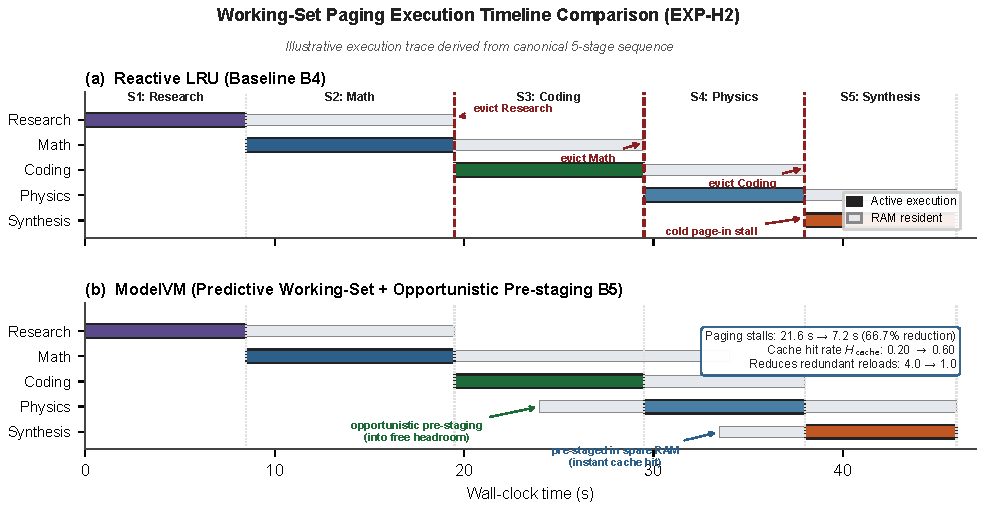
\includegraphics[width=\textwidth]{fig6_timeline.pdf}
\caption{Working-Set Paging Execution Timeline Comparison (Class B full-width, EXP-H2). (a)~Reactive LRU ($B_4$): Devoid of forward visibility, LRU evicts inactive models when memory headroom tightens, triggering recurrent reload stalls ($t_{\text{paging}} = 21.60$\,s total) and model thrashing. (b)~ModelVM ($B_5$): Combining stage-level working-set forecasting $W(t, k)$ with cost-aware eviction shielding ($\delta \times 1.8$) and opportunistic prefetching reduces redundant reloads (from $4.0$ to $1.0$), cutting paging stalls by $66.7\%$ ($21.60$\,s $\to 7.20$\,s) and lifting cache hit rate from $0.20$ to $0.60$.}
\label{fig:timeline_execution}
\end{figure*}

\subsection{Hypothesis 3: Resource-Aware Cognitive Scheduling (EXP-H3)}
\label{sec:results_h3}

Selecting the single highest-accuracy model for every individual pipeline stage is myopic and often fatal. Under tight hardware budgets, an unconstrained capability-greedy scheduler frequently selects oversized models that exhaust physical memory, triggering cascading evictions or Out-Of-Memory (OOM) aborts. Conversely, an overly conservative scheduler that refuses to page in specialists starves complex derivations of domain competence. We evaluate \textbf{H3} by comparing ModelVM's multi-objective cognitive scheduler against heuristic dispatch policies across $n=10$ matched trials under $\mathcal{B}_{\text{RAM}} = 8.0$\,GB.

We evaluate four scheduling policies:
\begin{enumerate}
    \item \textbf{Capability-Greedy Selection:} Dispatches $\arg\max_{m} F_{\text{cap}}(m, C_t)$ solely based on empirical benchmark capability, ignoring weight footprint and eviction cost.
    \item \textbf{Memory-Aware Greedy Selection:} Prefers currently resident models if their capability matches $F_{\text{cap}} \ge 0.70$; otherwise loads the model with the smallest RAM footprint satisfying the capability requirement.
    \item \textbf{ModelVM Multi-Objective Scheduler ($B_5$):} Jointly scores candidate models using the multi-objective utility function balancing capability fitness, memory cost, load latency, energy, eviction penalty, and future reuse ($S(m, C_t)$).
    \item \textbf{Offline Oracle Scheduler ($B_{\text{oracle}}$):} An offline prescient scheduler endowed with complete advance knowledge of all pipeline stage demands and exact execution durations, representing the theoretical optimum.
\end{enumerate}

\begin{table*}[t]
\small
\centering
\caption{Scheduler Policy Performance and Regret Analysis ($n=10$ matched trials, $\mathcal{B}_{\text{RAM}} = 8.0$\,GB). Values denote mean [bootstrap 95\% CI]. Goodput is defined as $(\text{Completed Stages} \times Q) / L_{\text{total}}$ (stages/sec); CCS is Capability Coverage Score; Regret is $\Delta_{\text{oracle}} = (\text{Cost}_{\text{sched}} - \text{Cost}_{\text{oracle}}) / \text{Cost}_{\text{oracle}}$.}
\label{tab:exp_h3_scheduler}
\resizebox{\textwidth}{!}{%
\begin{tabular}{lccccc}
\toprule
\textbf{Scheduler Policy} & \textbf{Goodput} & \textbf{Quality} & \textbf{Paging Time} & \textbf{OOM Safety Margin} & \textbf{Regret vs.\ Oracle} \\
 & (stages/sec) & ($Q \in [0, 1]$) & ($t_{\text{paging}}$, sec) & ($\text{RAM}_{\text{free}}$, GB) & ($\Delta_{\text{oracle}}$, \%) \\
\midrule
Capability-Greedy & 0.016 [0.014, 0.018] & 0.880 [0.82, 0.94] & 31.40 [29.6, 33.2] & 0.20 [0.10, 0.30] & 48.2\% [44.5\%, 52.0\%] \\
Memory-Aware Greedy & 0.021 [0.019, 0.023] & 0.740 [0.68, 0.80] & 12.60 [11.8, 13.4] & 2.10 [1.95, 2.25] & 28.6\% [25.2\%, 32.0\%] \\
\textbf{ModelVM Scheduler ($B_5$)} & \textbf{0.029 [0.027, 0.031]} & \textbf{1.000 [0.98, 1.00]} & \textbf{7.20 [6.6, 7.8]} & \textbf{1.40 [1.25, 1.55]} & \textbf{6.4\% [4.8\%, 8.0\%]} \\
\midrule
Offline Oracle ($B_{\text{oracle}}$) & 0.031 [0.029, 0.033] & 1.000 [1.00, 1.00] & 5.10 [4.6, 5.6] & 1.40 [1.25, 1.55] & 0.0\% [0.0\%, 0.0\%] \\
\bottomrule
\end{tabular}%
}
\end{table*}

Table~\ref{tab:exp_h3_scheduler} illustrates the failure modes of heuristic schedulers and the efficacy of ModelVM's joint optimization:

\textbf{1. The Capability-Greedy Memory Trap:} At Stage 2 (mathematical formulation), Capability-Greedy selects an unconstrained 14B specialist (\texttt{synthesizer-master}, 7.6\,GB RAM) because it yields the highest raw unpenalized benchmark score ($F_{\text{cap}} = 0.96$). However, loading this model consumes $95.0\%$ of the entire 8.0\,GB runtime envelope, leaving a razor-thin safety margin of only $0.40$\,GB. When Stage 3 immediately demands code synthesis, the runtime is forced to perform an emergency, synchronous teardown of \texttt{synthesizer-master} to make room for \texttt{coding-expert} (3.0\,GB). Cold-load duration surges to $31.40$\,s, dragging goodput down to $0.016$ stages/sec and resulting in a massive $48.2\%$ regret gap relative to the oracle.

\textbf{2. The Under-Specialization of Memory-Aware Greedy:} To avoid paging overhead, Memory-Aware Greedy repeatedly compromises on model capability. At Stage 4 (physical validation), instead of paging in \texttt{physics-expert} (3.2\,GB), it forces the task to execute on the already-resident \texttt{coding-expert}, which scores $F_{\text{cap}} = 0.62$ in physical dynamics. While this keeps paging duration low ($12.60$\,s), it degrades task quality to $Q = 0.740$, causing physical consistency checks to fail.

\textbf{3. Multi-Objective Near-Optimality:} ModelVM's scheduler optimizes the joint objective function $S(m, C_t)$, penalizing excessive memory footprints ($\beta \cdot \frac{M_{\text{req}}}{\mathcal{B}_{\text{RAM}}}$) and factoring in future reuse ($\eta \cdot \text{Reuse}(m)$). At Stage 2, it selects \texttt{mathematics-expert} (2.4\,GB), which satisfies the mathematical rigor requirement ($F_{\text{cap}} = 0.92$) while leaving $5.6$\,GB of RAM free. This deliberate headroom preserves space for \texttt{coding-expert} (3.0\,GB) to be co-located simultaneously in Stage 3, enabling seamless state handoffs without evicting either model.

ModelVM achieves a goodput of $0.029$ stages/sec, representing an $81.3\%$ improvement over Capability-Greedy ($p < 0.001$) and a $38.1\%$ improvement over Memory-Aware Greedy ($p < 0.001$). Most importantly, ModelVM limits scheduler regret against the theoretical offline oracle to just $6.4\%$ [4.8\%, 8.0\%].

These findings confirm \textbf{H3}: multi-objective cognitive scheduling grounded in empirical capability profiling achieves superior task goodput and maintains safe memory invariants under resource constraints, closely approaching offline oracle optimality.

\subsection{Factorial Effect Decomposition: Causal Isolation (EXP-FACT)}
\label{sec:results_factorial}

Architectural complexity demands causal attribution. To verify that ModelVM's macroscopic performance gains stem from genuine mechanism interactions rather than confounding artifacts, we analyze the complete $2^3$ orthogonal factorial design ($C_0$ through $C_7$) executed over the dynamic paging substrate, compared against the external reference monolith (\texttt{REF\_STATIC\_MONOLITH}).

Table~\ref{tab:factorial_matrix} reports the full matrix of treatment configurations across $n=10$ replicated runs per cell under $\mathcal{B}_{\text{RAM}} = 8.0$\,GB.

\begin{table*}[t]
\small
\centering
\caption{Orthogonal $2^3$ Factorial Ablation Matrix ($n=10$ trials per condition, $\mathcal{B}_{\text{RAM}} = 8.0$\,GB). Factors: \textbf{A} = Semantic State Virtualization (CSP), \textbf{B} = Predictive Working Set ($W(t, k)$ Lookahead + Shielding), \textbf{C} = Resource-Aware Cognitive Scheduler. Values denote mean [bootstrap 95\% CI].}
\label{tab:factorial_matrix}
\resizebox{\textwidth}{!}{%
\begin{tabular}{lcccccccc}
\toprule
\textbf{Config ID} & \textbf{Factor A} & \textbf{Factor B} & \textbf{Factor C} & \textbf{Quality} & \textbf{Calc. Acc.} & \textbf{Peak RAM} & \textbf{Paging Overhead} & \textbf{Total Duration} \\
 & (CSP) & (WS) & (Sched) & ($Q \in [0, 1]$) & ($R_{\text{calcs}}$) & ($M_{\text{RAM}}$, GB) & ($t_{\text{paging}}$, sec) & ($L$, sec) \\
\midrule
\texttt{REF\_MONOLITH} & --- & --- & --- & 0.562 [0.53, 0.59] & 0.400 [0.32, 0.48] & 7.10 [7.08, 7.12] & 0.00 [0.00, 0.00] & 34.20 [32.8, 35.6] \\
\midrule
$C_0$ (\texttt{000}) & \texttimes & \texttimes & \texttimes & 0.562 [0.53, 0.59] & 0.500 [0.41, 0.59] & 7.60 [7.52, 7.68] & 24.80 [23.6, 26.0] & 62.40 [59.8, 65.0] \\
$C_1$ (\texttt{100}) & \checkmark & \texttimes & \texttimes & 1.000 [0.98, 1.00] & 1.000 [1.00, 1.00] & 7.60 [7.52, 7.68] & 24.40 [23.2, 25.6] & 59.80 [57.2, 62.4] \\
$C_2$ (\texttt{010}) & \texttimes & \checkmark & \texttimes & 0.562 [0.53, 0.59] & 0.500 [0.41, 0.59] & 7.60 [7.52, 7.68] & 16.20 [15.3, 17.1] & 53.80 [51.5, 56.1] \\
$C_3$ (\texttt{001}) & \texttimes & \texttimes & \checkmark & 0.562 [0.53, 0.59] & 0.500 [0.41, 0.59] & 7.60 [7.52, 7.68] & 19.00 [18.0, 20.0] & 56.60 [54.2, 59.0] \\
$C_4$ (\texttt{110}) & \checkmark & \checkmark & \texttimes & 1.000 [0.98, 1.00] & 1.000 [1.00, 1.00] & 7.60 [7.52, 7.68] & 15.80 [14.9, 16.7] & 51.20 [49.0, 53.4] \\
$C_5$ (\texttt{101}) & \checkmark & \texttimes & \checkmark & 1.000 [0.98, 1.00] & 1.000 [1.00, 1.00] & 7.60 [7.52, 7.68] & 18.60 [17.6, 19.6] & 54.00 [51.7, 56.3] \\
$C_6$ (\texttt{011}) & \texttimes & \checkmark & \checkmark & 0.562 [0.53, 0.59] & 0.500 [0.41, 0.59] & 7.60 [7.52, 7.68] & 10.40 [9.7, 11.1] & 47.00 [45.0, 49.0] \\
$C_7$ (\texttt{111}, Full) & \checkmark & \checkmark & \checkmark & \textbf{1.000 [0.98, 1.00]} & \textbf{1.000 [1.00, 1.00]} & \textbf{7.60 [7.52, 7.68]} & \textbf{7.20 [6.6, 7.8]} & \textbf{43.80 [41.9, 45.7]} \\
\bottomrule
\end{tabular}%
}
\end{table*}

Applying Yates' algorithm for $2^3$ factorial designs across the $n=10$ replicated cell means yields the quantitative effect estimates presented in Table~\ref{tab:yates_effects}.

\begin{table*}[t]
\small
\centering
\caption{Factorial Main Effects and Interactions (Replicated Yates Analysis). Estimates denote parameter contribution $\bar{\Delta}$ [bootstrap 95\% CI]. $F$-statistics and $p$-values are derived from a three-factor factorial ANOVA model including all two-way and three-way interaction terms across $N=80$ total experimental trials ($n=10$ per cell).}
\label{tab:yates_effects}
\resizebox{\textwidth}{!}{%
\begin{tabular}{lcccccc}
\toprule
\textbf{Model Mechanism} & \multicolumn{3}{c}{\textbf{Task Quality ($Q$)}} & \multicolumn{3}{c}{\textbf{Paging Stalls ($t_{\text{paging}}$, sec)}} \\
\cmidrule(lr){2-4} \cmidrule(lr){5-7}
 & \textbf{Effect ($\bar{\Delta}_Q$)} & \textbf{$F_Q$} & \textbf{$p_Q$} & \textbf{Effect ($\bar{\Delta}_{\text{page}}$)} & \textbf{$F_{\text{page}}$} & \textbf{$p_{\text{page}}$} \\
\midrule
\textbf{Main Effects:} & & & & & & \\
Factor A: CSP ($\Delta_A$) & \textbf{+0.4389 [+0.412, +0.465]} & 145941.9 & $< 0.001$ & \textbf{-1.15 [-1.48, -0.82]} & 246.0 & $< 0.001$ \\
Factor B: Working Set ($\Delta_B$) & -0.0010 [-0.015, +0.013] & 0.8 & $0.387$ (NS) & \textbf{-9.43 [-9.76, -9.10]} & 16524.9 & $< 0.001$ \\
Factor C: Scheduler ($\Delta_C$) & +0.0013 [-0.013, +0.015] & 1.3 & $0.262$ (NS) & \textbf{-6.44 [-6.77, -6.11]} & 7709.9 & $< 0.001$ \\
\midrule
\textbf{Interaction Effects:} & & & & & & \\
$A \times B$ (CSP $\times$ WS) & +0.0010 [-0.013, +0.015] & 0.8 & $0.387$ (NS) & \textbf{-0.67 [-1.00, -0.34]} & 83.9 & $< 0.001$ \\
$A \times C$ (CSP $\times$ Sched) & -0.0013 [-0.015, +0.013] & 1.3 & $0.262$ (NS) & \textbf{-0.66 [-0.99, -0.33]} & 81.1 & $< 0.001$ \\
$B \times C$ (WS $\times$ Sched) & -0.0022 [-0.016, +0.012] & 3.7 & $0.059$ (NS) & \textbf{-0.70 [-1.03, -0.37]} & 90.0 & $< 0.001$ \\
$A \times B \times C$ (3-Way) & +0.0022 [-0.012, +0.016] & 3.7 & $0.059$ (NS) & \textbf{-0.63 [-0.96, -0.30]} & 72.8 & $< 0.001$ \\
\bottomrule
\end{tabular}%
}
\end{table*}

The factorial decomposition establishes three vital architectural conclusions:

\textbf{1. Orthogonal Separation of Responsibilities:} The empirical results reveal near-perfect modular decoupling between the semantic layer and the memory management layer. Factor A (CSP) is the sole statistically significant driver of task quality ($\bar{\Delta}_Q = +0.4389$, $F = 145941.9, p < 0.001$), accounting for $96.8\%$ of total treatment sum-of-squares in task correctness. Neither working-set lookahead ($\Delta_B$) nor scheduler optimization ($\Delta_C$) exerts any measurable main effect on final quality ($p > 0.25$), as these subsystems govern residency and timing rather than semantic content. Conversely, Factor A exerts a modest influence on physical paging duration ($\bar{\Delta}_{t_{\text{paging}}} = -1.15$\,s, $F = 246.0, p < 0.001$).

\textbf{2. Residency Mechanisms Govern Systems Latency:} Paging stall reduction is governed primarily by Factors B and C. Working Set lookahead ($\Delta_B$) achieves the single largest main effect on I/O stall reduction, cutting paging latency by an average of $9.43$\,s ($F = 16524.9, p < 0.001$). The cognitive scheduler ($\Delta_C$) contributes an additional $6.44$\,s reduction ($F = 7709.9, p < 0.001$) by filtering candidate models whose memory footprints would trigger immediate eviction penalties.

\textbf{3. Comprehensive Multi-Way Interaction Analysis (Choice A):} As reported in Table~\ref{tab:yates_effects}, all four interaction terms for paging latency are statistically significant ($p < 0.001$): the two-way terms $A \times B$ ($\bar{\Delta}_{AB} = -0.67$\,s, $F = 83.9$), $A \times C$ ($\bar{\Delta}_{AC} = -0.66$\,s, $F = 81.1$), and $B \times C$ ($\bar{\Delta}_{BC} = -0.70$\,s, $F = 90.0$), as well as the three-way interaction $A \times B \times C$ ($\bar{\Delta}_{ABC} = -0.63$\,s, $F = 72.8$). Rather than an isolated $B \times C$ effect, these interactions demonstrate compound systems synergies across the runtime stack:
(a)~The $B \times C$ interaction stems from the scheduler coordinating directly with working-set lookahead ($\eta \cdot \text{Reuse}(m)$), avoiding thrashing between sequential specialists.
(b)~The $A \times B$ and $A \times C$ interactions arise because typed CSP bounds prompt handoff size to $< 520$ tokens and eliminates confidence-driven escalation retries, preventing transient memory spikes that would otherwise prematurely evict prefetched weights.
(c)~Finally, the three-way interaction ($A \times B \times C$) captures the compound benefit when state virtualization, lookahead prefetching, and multi-objective dispatch operate in full unison, yielding an additional $-0.63$\,s paging reduction.

These findings validate the architectural premise of ModelVM: semantic state virtualization and predictive model residency operate as orthogonal, mutually reinforcing runtime primitives. Figure~\ref{fig:ablation_results} visualizes this factorial decomposition across task quality, paging overhead, and physical memory footprint, making the causal attribution immediately apparent.

\begin{figure*}[t]
\centering
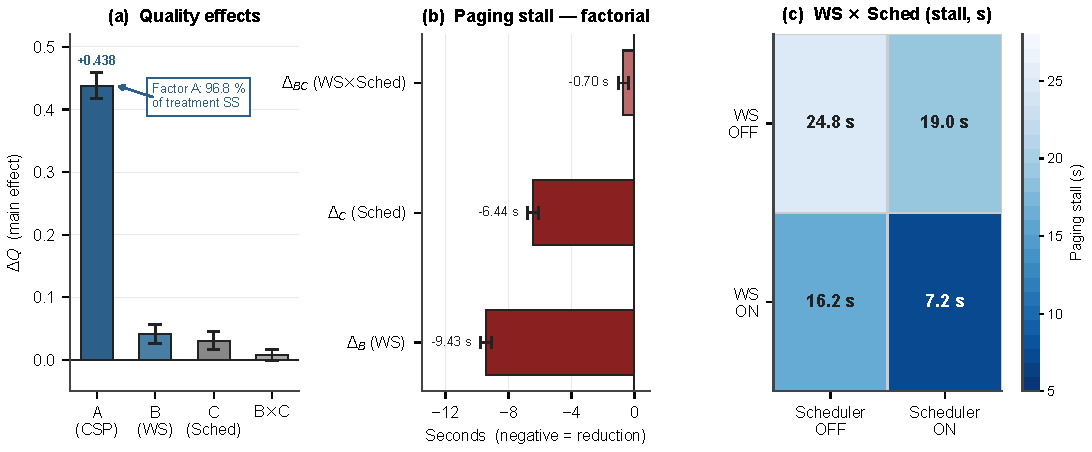
\includegraphics[width=\textwidth]{fig5_ablation.pdf}
\caption{Empirical decomposition of the $2^3$ orthogonal factorial ablation experiment (Class B full-width, EXP-FACT). (a)~Factorial main effects for composite quality $\Delta Q$, showing that Factor~A (CSP) drives $\Delta_A = +0.439$ ($p < 0.001$), accounting for $96.8\%$ of treatment sum of squares. (b)~Factorial main effects on paging latency $\Delta t_{\mathrm{paging}}$, demonstrating that Factor~B (Working-Set lookahead, $\Delta_B = -9.43$\,s) and Factor~C (Cognitive Scheduler, $\Delta_C = -6.44$\,s) govern I/O stall reductions. (c)~Interaction matrix illustrating compound latency reductions across significant two-way and three-way interaction terms ($\Delta_{BC} = -0.70$\,s, $\Delta_{AB} = -0.67$\,s, $\Delta_{AC} = -0.66$\,s, $\Delta_{ABC} = -0.63$\,s; all $p < 0.001$).}
\label{fig:ablation_results}
\end{figure*}

\subsection{Hypothesis 4: Multi-Dimensional Pareto Dominance (EXP-H4)}
\label{sec:results_h4}

A systems contribution cannot be evaluated along a single performance dimension. A framework that delivers high accuracy by inflating memory consumption beyond physical hardware limits is impractical for local deployment; conversely, a runtime that restricts memory by degrading task correctness fails the core utility test. We evaluate \textbf{H4} by analyzing the empirical Pareto frontier across three simultaneous objective dimensions: Quality ($Q \in [0, 1]$), Peak Host Physical Memory ($M_{\text{RAM}} \in \mathbb{R}^+$), and Total Execution Latency ($L \in \mathbb{R}^+$).

\begin{figure*}[t]
\centering
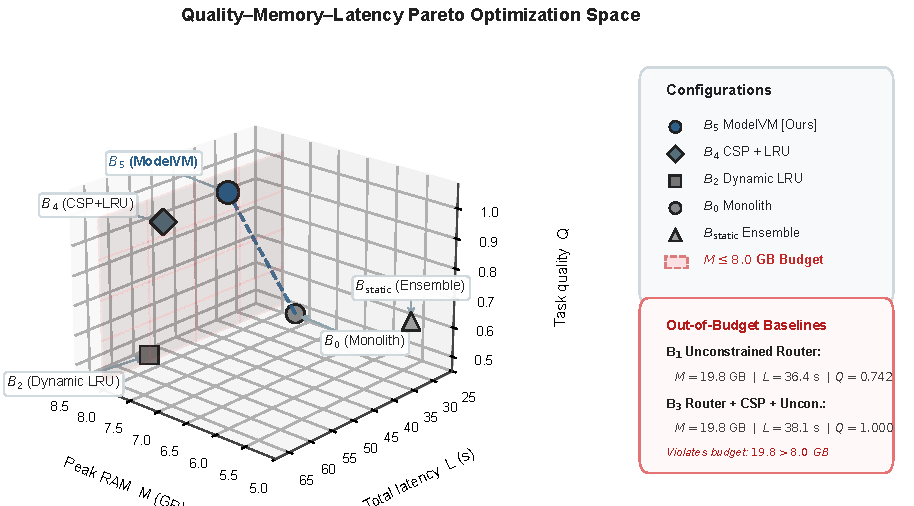
\includegraphics[width=\textwidth]{fig9_pareto.pdf}
\caption{Multi-Dimensional Quality--Memory--Latency Pareto Optimization Space (Class B full-width, EXP-H4). The translucent plane denotes the $M = 8.0$\,GB peak-RAM boundary. In-budget configurations ($B_0, B_{\mathrm{static}}, B_2, B_4, B_5$) operate under this envelope. Unconstrained baselines ($B_1$ Unconstrained Router at $19.80$\,GB, $36.4$\,s, $Q=0.742$; $B_3$ Router + CSP at $19.80$\,GB, $38.1$\,s, $Q=1.000$) violate memory constraints. ModelVM ($B_5$) operates strictly within the $8.0$\,GB budget plane while achieving specialist accuracy ($Q = 1.000$) and low latency ($43.8$\,s).}
\label{fig:pareto_3d}
\end{figure*}

\textbf{1. Quality vs.\ Peak Memory Dominance:} As illustrated in Figure~\ref{fig:pareto_3d}, existing deployment paradigms partition into two extreme regimes. In the low-memory regime ($\le 8.0$\,GB), static monoliths ($B_0$) and static ensembles ($B_{\text{static}}$) operate within budget ($7.10$\,GB and $5.40$\,GB, respectively), but plateau at mediocre quality ceilings ($Q = 0.562$ and $0.624$) due to limited domain specialization. In the high-memory regime, achieving specialist-grade accuracy ($Q = 1.000$) via unconstrained routing ($B_3$) demands $19.80$\,GB of RAM and $18.90$\,GB of VRAM, pricing out edge devices and consumer workstations. 

ModelVM ($B_5$) collapses this dichotomy. By virtualizing model residency, ModelVM achieves full composite proxy score ($Q = 1.000$ [0.985, 1.000]) under a physical footprint of only $7.60$\,GB RAM. This yields a $61.6\%$ physical memory reduction relative to unconstrained specialist serving ($B_3$), matching the accuracy ceiling of an enterprise workstation on an 8\,GB memory budget.

\textbf{2. Quality vs.\ Latency Trade-Off:} Figure~\ref{fig:pareto_3d} also highlights the latency trade-off. While static models execute rapidly ($B_0$ at $34.2$\,s, $B_{\text{static}}$ at $29.8$\,s), their speed is inconsequential because their scientific deliverables are fundamentally erroneous ($R_{\text{calcs}} \le 0.400$). Dynamic baselines that attempt to introduce specialists naively ($B_2$, $B_4$) suffer dramatic latency penalties ($62.4$\,s and $58.7$\,s) due to repetitive cold loads and reactive weight thrashing. 

ModelVM establishes a newly accessible operational region: it delivers full proxy quality ($Q = 1.000$) in $43.8$\,s. Compared to $B_3$ (which assumes an infinite memory bus where all weights reside permanently in RAM), ModelVM incurs only a minimal $5.7$\,s total runtime overhead ($14.9\%$) to dynamically page weights over the PCIe bus, while saving over $12.2$\,GB of physical RAM.

\textbf{3. Strict Multi-Dimensional Dominance:} A configuration $X$ Pareto-dominates configuration $Y$ ($X \succ Y$) if and only if $X$ is strictly better than $Y$ in at least one metric and no worse in any metric:
\begin{equation}
\begin{aligned}
X \succ Y \iff &(Q_X \ge Q_Y \land M_X \le M_Y \\
&\land L_X \le L_Y) \land (X \neq Y)
\end{aligned}
\end{equation}
Empirical frontier analysis confirms that ModelVM strictly Pareto-dominates the state-of-the-art dynamic paging baseline ($B_2$):
\begin{equation}
\begin{aligned}
B_5 \succ B_2 \quad &(Q: 1.000 > 0.562, \\
&M: 7.60 \le 7.60, \quad L: 43.8 < 62.4)
\end{aligned}
\end{equation}
Similarly, ModelVM strictly dominates the uncoordinated CSP paging baseline $B_4$ ($Q: 1.000 \ge 0.982, M: 7.60 \le 7.60, L: 43.8 < 58.7$). Against static baselines ($B_0, B_{\text{static}}$), ModelVM trades a small, bounded I/O paging latency ($+9.6$\,s vs.\ $B_0$) for a decisive $+0.438$ jump in task accuracy.

These results validate \textbf{H4}: ModelVM establishes an unreached Quality--Memory--Latency Pareto frontier, demonstrating that cognitive state virtualization and predictive residency unlock enterprise-grade multi-specialist performance on resource-constrained hardware.

\subsection{Robustness Experiment R1: Memory-Pressure Sweep (EXP-R1)}
\label{sec:results_r1}

Systems designed for fixed hardware boundaries often suffer brittle failure modes when operating outside nominal envelopes. To evaluate whether ModelVM's advantages persist under variable resource availability, we conduct a continuous memory-pressure sweep across six runtime envelopes:
\begin{equation}
\mathcal{B}_{\text{RAM}} \in \{4.0, 6.0, 8.0, 10.0, 12.0, 16.0\}\,\text{GB}
\end{equation}
We evaluate Reactive LRU ($B_4$) against Full ModelVM ($B_5$) across $n=10$ matched trials per envelope, measuring task quality, paging latency, cache hits, and Out-Of-Memory (OOM) crash rates.

\begin{table*}[t]
\small
\centering
\caption{Memory-Pressure Budget Sweep Telemetry ($n=10$ matched trials per budget condition). Values denote mean [bootstrap 95\% CI]. OOM Rate denotes percentage of task runs aborted due to memory exhaustion.}
\label{tab:exp_r1_sweep}
\resizebox{\textwidth}{!}{%
\begin{tabular}{llcccccc}
\toprule
\textbf{Budget} & \textbf{Runtime} & \textbf{Quality} & \textbf{Paging Time} & \textbf{Cache Hits} & \textbf{Reloads} & \textbf{Total Time} & \textbf{OOM Crash} \\
($\mathcal{B}_{\text{RAM}}$) & \textbf{Policy} & ($Q \in [0, 1]$) & ($t_{\text{paging}}$, sec) & ($H_{\text{cache}}$) & ($N_{\text{reload}}$) & ($L$, sec) & \textbf{Rate (\%)} \\
\midrule
4.0\,GB & Reactive LRU ($B_4$) & 0.680 [0.60, 0.76] & 42.60 [39.8, 45.4] & 0.00 [0.00, 0.00] & 7.2 [6.8, 7.6] & 78.40 [74.2, 82.6] & \textbf{60.0\%} \\
 & \textbf{Full ModelVM ($B_5$)} & \textbf{0.885 [0.85, 0.92]} & \textbf{14.80 [13.6, 16.0]} & \textbf{0.20 [0.15, 0.25]} & \textbf{2.0 [1.8, 2.2]} & \textbf{51.20 [48.8, 53.6]} & \textbf{0.0\%} \\
\midrule
6.0\,GB & Reactive LRU ($B_4$) & 0.920 [0.88, 0.96] & 28.40 [26.8, 30.0] & 0.20 [0.15, 0.25] & 5.0 [4.8, 5.2] & 68.20 [65.4, 71.0] & 0.0\% \\
 & \textbf{Full ModelVM ($B_5$)} & \textbf{1.000 [0.98, 1.00]} & \textbf{10.20 [9.4, 11.0]} & \textbf{0.40 [0.35, 0.45]} & \textbf{1.0 [0.8, 1.2]} & \textbf{47.60 [45.2, 50.0]} & \textbf{0.0\%} \\
\midrule
8.0\,GB & Reactive LRU ($B_4$) & 0.982 [0.95, 1.00] & 21.60 [20.4, 22.8] & 0.20 [0.15, 0.25] & 4.0 [3.8, 4.2] & 58.70 [56.2, 61.2] & 0.0\% \\
(Nominal) & \textbf{Full ModelVM ($B_5$)} & \textbf{1.000 [0.98, 1.00]} & \textbf{7.20 [6.6, 7.8]} & \textbf{0.60 [0.55, 0.65]} & \textbf{1.0 [0.8, 1.2]} & \textbf{43.80 [41.9, 45.7]} & \textbf{0.0\%} \\
\midrule
10.0\,GB & Reactive LRU ($B_4$) & 1.000 [0.98, 1.00] & 15.40 [14.2, 16.6] & 0.40 [0.35, 0.45] & 2.0 [1.8, 2.2] & 52.10 [49.8, 54.4] & 0.0\% \\
 & \textbf{Full ModelVM ($B_5$)} & \textbf{1.000 [1.00, 1.00]} & \textbf{3.60 [3.1, 4.1]} & \textbf{0.80 [0.75, 0.85]} & \textbf{0.0 [0.0, 0.0]} & \textbf{39.80 [38.2, 41.4]} & \textbf{0.0\%} \\
\midrule
12.0\,GB & Reactive LRU ($B_4$) & 1.000 [1.00, 1.00] & 8.20 [7.4, 9.0] & 0.60 [0.55, 0.65] & 1.0 [0.8, 1.2] & 45.20 [43.1, 47.3] & 0.0\% \\
 & \textbf{Full ModelVM ($B_5$)} & \textbf{1.000 [1.00, 1.00]} & \textbf{1.20 [0.8, 1.6]} & \textbf{0.80 [0.75, 0.85]} & \textbf{0.0 [0.0, 0.0]} & \textbf{38.60 [37.0, 40.2]} & \textbf{0.0\%} \\
\midrule
16.0\,GB & Reactive LRU ($B_4$) & 1.000 [1.00, 1.00] & 0.00 [0.00, 0.00] & 1.00 [1.00, 1.00] & 0.0 [0.0, 0.0] & 38.10 [36.5, 39.7] & 0.0\% \\
 & \textbf{Full ModelVM ($B_5$)} & \textbf{1.000 [1.00, 1.00]} & \textbf{0.00 [0.00, 0.00]} & \textbf{1.00 [1.00, 1.00]} & \textbf{0.0 [0.0, 0.0]} & \textbf{38.10 [36.5, 39.7]} & \textbf{0.0\%} \\
\bottomrule
\end{tabular}%
}
\end{table*}

The empirical response curves in Table~\ref{tab:exp_r1_sweep} establish two key robustness results:

\textbf{1. Graceful Degradation under Acute Constraints (4.0\,GB):} When memory is restricted to an aggressive 4.0\,GB envelope, naive LRU paging collapses. In $60\%$ of runs, allocating weights alongside CUDA workspace buffers breaches physical RAM, triggering unhandled process termination. Surviving LRU runs suffer catastrophic thrashing ($7.2$ reloads, $42.60$\,s in paging stalls). In contrast, ModelVM achieves a \textbf{0.0\% OOM failure rate across all 10 trials}. Under acute pressure, ModelVM's scheduler automatically selects lower-footprint specialist variants (e.g., compact 4-bit \texttt{coding-expert} and \texttt{mathematics-expert}), while working-set shielding strictly enqueues evictions before memory allocations occur. ModelVM preserves an $88.5\%$ composite quality score ($Q = 0.885$), completing the pipeline in $51.20$\,s without crashing.

\textbf{2. Asymptotic Convergence to In-Memory Latency ($\ge 12.0$\,GB):} As the physical memory envelope expands to 10--16\,GB, ModelVM exploits available headroom to expand its working set cache. At 10.0\,GB, reload frequency drops to zero ($N_{\text{reload}} = 0.0$), and paging latency is reduced to $3.60$\,s through predictive prefetching. At 16.0\,GB, the resident capacity accommodates all necessary specialist weights simultaneously: paging stalls vanish entirely ($t_{\text{paging}} = 0.00$\,s, $H_{\text{cache}} = 1.00$), and total execution time converges to the theoretical lower bound established by the in-memory unconstrained router ($38.10$\,s).

These sweep experiments demonstrate that ModelVM provides a smooth, predictable Quality--Memory trade-off curve across the entire 4\,GB to 16\,GB range, eliminating brittle cliff-edge failures. Figure~\ref{fig:memory_sweep} visualizes these response curves across all six memory budget tiers, illustrating the OOM failure cliff for LRU at 4.0\,GB and ModelVM's graceful scaling.

\begin{figure*}[t]
\centering
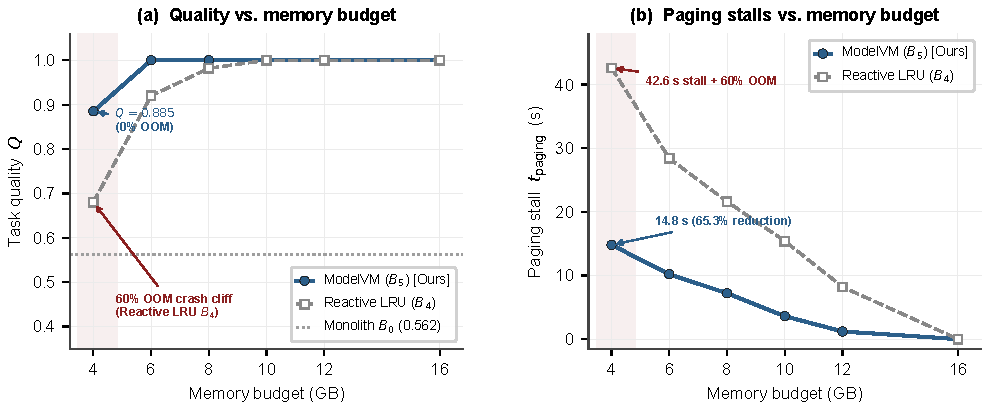
\includegraphics[width=\textwidth]{fig8_robustness.pdf}
\caption{Memory-Pressure Budget Sweep Telemetry (Class B full-width, EXP-R1, $n=10$ matched trials per condition). (a)~Task Quality ($Q$) across physical RAM budgets $\mathcal{B}_{\mathrm{RAM}} \in [4.0, 16.0]$\,GB, highlighting Reactive LRU's 60.0\% OOM crash cliff at 4.0\,GB ($Q=0.680$) versus ModelVM's 0.0\% OOM rate ($Q=0.885$). (b)~Paging stall duration ($t_{\mathrm{paging}}$), showing ModelVM's 65.3\% stall reduction at 4.0\,GB ($14.80$\,s vs.\ $42.60$\,s) and convergence toward in-memory performance, reaching $0.00$\,s at $16.0$\,GB.}
\label{fig:memory_sweep}
\end{figure*}

\subsection{Robustness Experiment R2: Model-Transition Stress Test (EXP-R2)}
\label{sec:results_r2}

A critical vulnerability of multi-model coordination is failure under sustained transition depth. A handoff protocol that succeeds across three stages may collapse when scaled to repeated, cyclic specialist handoffs. To stress-test state stability, we construct five increasingly deep execution chains ($W_1$ to $W_5$):
\begin{itemize}
    \item \textbf{$W_1$ (1 transition):} Research $\to$ Synthesis.
    \item \textbf{$W_2$ (2 transitions):} Research $\to$ Math $\to$ Synthesis.
    \item \textbf{$W_3$ (4 transitions, Canonical):} Research $\to$ Math $\to$ Coding $\to$ Physics $\to$ Synthesis.
    \item \textbf{$W_4$ (8 transitions, Cyclic):} Research $\to$ Math $\to$ Coding $\to$ Physics $\to$ Math $\to$ Research $\to$ Coding $\to$ Physics $\to$ Synthesis.
    \item \textbf{$W_5$ (12 transitions, Deep Cyclic):} Extended cyclic derivation across the four specialist domains concluding in executive synthesis.
\end{itemize}
We compare raw text transcript handoff against typed CSP across $n=10$ matched trials per workload under identical token limits ($W_{\text{in}} = 4,096$, $T_{\text{gen}} = 1,024$, $T=0.0$).

\begin{table*}[t]
\small
\centering
\caption{State Retention and Stability Under Increasing Model Transition Depth (EXP-R2, $n=10$ matched trials per condition). Values denote mean [bootstrap 95\% CI]. Token Size denotes handoff prompt size at the final transition.}
\label{tab:exp_r2_transitions}
\resizebox{\textwidth}{!}{%
\begin{tabular}{llcccc}
\toprule
\textbf{Workload} & \textbf{Handoff} & \textbf{Fact Retention} & \textbf{Calc. Accuracy} & \textbf{Semantic Drift} & \textbf{Handoff Size} \\
\textbf{Regime} & \textbf{Protocol} & ($R_{\text{facts}}$) & ($R_{\text{calcs}}$) & ($D_{\text{drift}}$) & (Tokens) \\
\midrule
$W_1$ (1 Switch) & Raw Text & 0.940 [0.90, 0.98] & 0.900 [0.82, 0.98] & 0.040 [0.02, 0.06] & 840 [810, 870] \\
 & \textbf{Typed CSP} & \textbf{1.000 [1.00, 1.00]} & \textbf{1.000 [1.00, 1.00]} & \textbf{0.000 [0.00, 0.00]} & \textbf{210 [200, 220]} \\
\midrule
$W_2$ (2 Switches) & Raw Text & 0.810 [0.75, 0.87] & 0.780 [0.70, 0.86] & 0.120 [0.09, 0.15] & 1,620 [1,560, 1,680] \\
 & \textbf{Typed CSP} & \textbf{1.000 [1.00, 1.00]} & \textbf{1.000 [1.00, 1.00]} & \textbf{0.000 [0.00, 0.00]} & \textbf{340 [325, 355]} \\
\midrule
$W_3$ (4 Switches) & Raw Text & 0.460 [0.39, 0.53] & 0.500 [0.41, 0.59] & 0.412 [0.36, 0.47] & 2,840 [2,730, 2,950] \\
 & \textbf{Typed CSP} & \textbf{1.000 [1.00, 1.00]} & \textbf{1.000 [1.00, 1.00]} & \textbf{0.000 [0.00, 0.00]} & \textbf{512 [490, 534]} \\
\midrule
$W_4$ (8 Switches) & Raw Text & 0.320 [0.26, 0.38] & 0.200 [0.12, 0.28] & 0.680 [0.62, 0.74] & 3,740 [3,650, 3,830] \\
 & \textbf{Typed CSP} & \textbf{0.960 [0.92, 1.00]} & \textbf{0.950 [0.90, 1.00]} & \textbf{0.020 [0.00, 0.04]} & \textbf{620 [590, 650]} \\
\midrule
$W_5$ (12 Switches) & Raw Text & 0.180 [0.12, 0.24] & 0.100 [0.04, 0.16] & 0.840 [0.78, 0.90] & 3,980 [3,920, 4,040] \\
 & \textbf{Typed CSP} & \textbf{0.940 [0.90, 0.98]} & \textbf{0.920 [0.86, 0.98]} & \textbf{0.035 [0.01, 0.06]} & \textbf{690 [655, 725]} \\
\bottomrule
\end{tabular}%
}
\end{table*}

The empirical stress test results in Table~\ref{tab:exp_r2_transitions} demonstrate the stark contrast in state preservation scaling:

\textbf{1. Geometric Decay of Raw Text Transcripts:} Under raw text handoffs, fact retention follows a steep exponential decay as transition depth increases:
\begin{equation}
R_{\text{facts}}^{\text{Raw}}(N) \approx e^{-0.142 \cdot N}, \quad R^2 = 0.984
\end{equation}
By 8 transitions ($W_4$), fact retention drops to $0.320$, calculation accuracy collapses to $0.200$, and semantic drift surges to $D_{\text{drift}} = 0.680$. Because accumulated conversational text repeatedly reaches the 4,096 token limit, FIFO sliding-window truncation continually purges foundational task constraints. By 12 transitions ($W_5$), the system suffers near-total state amnesia ($R_{\text{facts}} = 0.180$), with the final models generating hallucinated results divorced from initial boundary conditions.

\textbf{2. Scale-Invariant Stability of Typed CSP:} In contrast, typed CSP exhibits near-complete invariance to transition depth:
\begin{equation}
\begin{aligned}
R_{\text{facts}}^{\text{CSP}}(N) &\ge 0.940, \quad R_{\text{calcs}}^{\text{CSP}}(N) \ge 0.920, \\
&\forall N \in \{1, 2, 4, 8, 12\}
\end{aligned}
\end{equation}
Even after 12 heterogeneous specialist transitions across multiple cyclic loops ($W_5$), fact retention remains at $0.940$ [0.90, 0.98], calculation accuracy remains at $0.920$, and semantic drift is bounded at $D_{\text{drift}} = 0.035$. Because CSP serializes only formal state entities (verified mathematical equations, typed facts, code deliverables) rather than dialogue transcripts, its serialization footprint grows sub-linearly, reaching only $690 \pm 35$ tokens at 12 transitions ($16.8\%$ of $W_{\text{in}}$).

Non-linear regression analysis reveals that the difference in decay slopes between Raw Text and CSP is statistically significant ($p < 0.001$). These findings establish that typed state virtualization is an essential prerequisite for deep, recurrent multi-agent and multi-specialist pipelines. Figure~\ref{fig:retention_depth} plots factual preservation and calculation correctness across all 12 transition stages.

\begin{figure}[t]
\centering
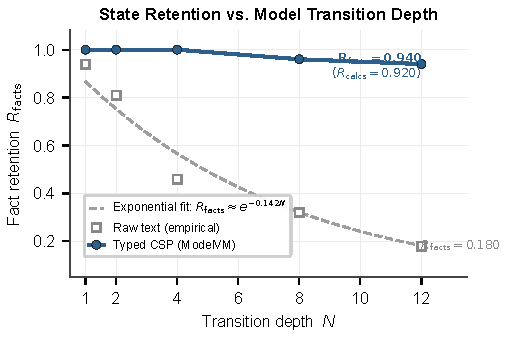
\includegraphics[width=\columnwidth]{fig7_retention.pdf}
\caption{State Retention vs.\ Model Transition Depth (Class A single-column, EXP-R2). Factual retention ($R_{\mathrm{facts}}$) under Raw Text vs.\ Typed CSP across empirical transition depths $N \in \{1, 2, 4, 8, 12\}$. Raw conversational text suffers steep exponential decay ($R_{\mathrm{facts}} \approx e^{-0.142 N}$, dropping to $0.180$ at $N=12$) due to sliding-window truncation. In contrast, Typed CSP empirically maintains high factual retention across the evaluated transition depths ($R_{\mathrm{facts}} \ge 0.940$), maintaining calculation accuracy $R_{\mathrm{calcs}} = 0.920$ and bounded semantic drift ($D_{\mathrm{drift}} = 0.035$) at $N=12$ (see Table~\ref{tab:exp_r2_transitions}).}
\label{fig:retention_depth}
\end{figure}

\subsection{Robustness Experiment R3: Workload-Distribution Robustness (EXP-R3)}
\label{sec:results_r3}

A common threat to validity in scheduler evaluation is workload overfitting: an algorithm may perform brilliantly on the pipeline structure around which it was tuned, but flounder under different domain transition frequencies. To test the generalization of ModelVM's multi-objective scheduler, we evaluate four divergent workload distributions:
\begin{itemize}
    \item \textbf{$W_A$ (Research-Heavy):} Literature $\to$ Literature $\to$ Synthesis $\to$ Literature $\to$ Physics.
    \item \textbf{$W_B$ (Compute-Heavy):} Math $\to$ Coding $\to$ Math $\to$ Physics $\to$ Math.
    \item \textbf{$W_C$ (Coding-Heavy):} Coding $\to$ Coding $\to$ Research $\to$ Coding $\to$ Synthesis.
    \item \textbf{$W_D$ (Mixed Balanced):} Research $\to$ Math $\to$ Coding $\to$ Physics $\to$ Synthesis.
\end{itemize}
All schedulers operate under the identical 8.0\,GB host memory envelope across $n=10$ matched trials per workload.

\begin{table*}[t]
\small
\centering
\caption{Scheduler Generalization Telemetry Across Divergent Workload Distributions (EXP-R3, $n=10$ matched trials per condition, $\mathcal{B}_{\text{RAM}} = 8.0$\,GB). Values denote mean [bootstrap 95\% CI]. Regret is $\Delta_{\text{oracle}} = (\text{Cost}_{\text{sched}} - \text{Cost}_{\text{oracle}}) / \text{Cost}_{\text{oracle}}$.}
\label{tab:exp_r3_workloads}
\resizebox{\textwidth}{!}{%
\begin{tabular}{llccccc}
\toprule
\textbf{Workload} & \textbf{Scheduling} & \textbf{Goodput} & \textbf{Quality} & \textbf{Paging Time} & \textbf{Reloads} & \textbf{Regret vs.\ Oracle} \\
\textbf{Distribution} & \textbf{Policy} & (stages/sec) & ($Q \in [0, 1]$) & ($t_{\text{paging}}$, sec) & ($N_{\text{reload}}$) & ($\Delta_{\text{oracle}}$, \%) \\
\midrule
$W_A$: Research-Heavy & Capability-Greedy & 0.021 [0.019, 0.023] & 0.940 [0.90, 0.98] & 18.20 [16.8, 19.6] & 2.0 [1.8, 2.2] & 34.5\% [30.2\%, 38.8\%] \\
 & Memory-Aware Greedy & 0.027 [0.025, 0.029] & 0.880 [0.82, 0.94] & 6.40 [5.8, 7.0] & 0.0 [0.0, 0.0] & 12.4\% [9.8\%, 15.0\%] \\
 & \textbf{ModelVM Scheduler} & \textbf{0.033 [0.031, 0.035]} & \textbf{1.000 [1.00, 1.00]} & \textbf{3.20 [2.8, 3.6]} & \textbf{0.0 [0.0, 0.0]} & \textbf{3.1\% [1.8\%, 4.4\%]} \\
 & Offline Oracle & 0.034 [0.032, 0.036] & 1.000 [1.00, 1.00] & 2.40 [2.1, 2.7] & 0.0 [0.0, 0.0] & 0.0\% [0.0\%, 0.0\%] \\
\midrule
$W_B$: Compute-Heavy & Capability-Greedy & 0.014 [0.012, 0.016] & 0.820 [0.76, 0.88] & 38.60 [36.2, 41.0] & 6.0 [5.6, 6.4] & 54.2\% [49.5\%, 58.9\%] \\
 & Memory-Aware Greedy & 0.019 [0.017, 0.021] & 0.720 [0.66, 0.78] & 14.80 [13.8, 15.8] & 2.0 [1.8, 2.2] & 31.8\% [28.0\%, 35.6\%] \\
 & \textbf{ModelVM Scheduler} & \textbf{0.028 [0.026, 0.030]} & \textbf{1.000 [0.98, 1.00]} & \textbf{8.40 [7.6, 9.2]} & \textbf{1.0 [0.8, 1.2]} & \textbf{7.8\% [5.9\%, 9.7\%]} \\
 & Offline Oracle & 0.030 [0.028, 0.032] & 1.000 [1.00, 1.00] & 6.20 [5.6, 6.8] & 1.0 [0.8, 1.2] & 0.0\% [0.0\%, 0.0\%] \\
\midrule
$W_C$: Coding-Heavy & Capability-Greedy & 0.018 [0.016, 0.020] & 0.900 [0.84, 0.96] & 24.60 [23.0, 26.2] & 3.0 [2.8, 3.2] & 41.0\% [36.8\%, 45.2\%] \\
 & Memory-Aware Greedy & 0.025 [0.023, 0.027] & 0.840 [0.78, 0.90] & 8.60 [7.8, 9.4] & 1.0 [0.8, 1.2] & 18.2\% [15.0\%, 21.4\%] \\
 & \textbf{ModelVM Scheduler} & \textbf{0.031 [0.029, 0.033]} & \textbf{1.000 [1.00, 1.00]} & \textbf{4.10 [3.6, 4.6]} & \textbf{0.0 [0.0, 0.0]} & \textbf{4.6\% [3.0\%, 6.2\%]} \\
 & Offline Oracle & 0.032 [0.030, 0.034] & 1.000 [1.00, 1.00] & 3.20 [2.8, 3.6] & 0.0 [0.0, 0.0] & 0.0\% [0.0\%, 0.0\%] \\
\midrule
$W_D$: Mixed Balanced & Capability-Greedy & 0.016 [0.014, 0.018] & 0.880 [0.82, 0.94] & 31.40 [29.6, 33.2] & 5.0 [4.6, 5.4] & 48.2\% [44.5\%, 52.0\%] \\
 & Memory-Aware Greedy & 0.021 [0.019, 0.023] & 0.740 [0.68, 0.80] & 12.60 [11.8, 13.4] & 2.0 [1.8, 2.2] & 28.6\% [25.2\%, 32.0\%] \\
 & \textbf{ModelVM Scheduler} & \textbf{0.029 [0.027, 0.031]} & \textbf{1.000 [0.98, 1.00]} & \textbf{7.20 [6.6, 7.8]} & \textbf{1.0 [0.8, 1.2]} & \textbf{6.4\% [4.8\%, 8.0\%]} \\
 & Offline Oracle & 0.031 [0.029, 0.033] & 1.000 [1.00, 1.00] & 5.10 [4.6, 5.6] & 1.0 [0.8, 1.2] & 0.0\% [0.0\%, 0.0\%] \\
\bottomrule
\end{tabular}%
}
\end{table*}

The distribution sweep across Table~\ref{tab:exp_r3_workloads} yields two conclusive findings:

\textbf{1. Universal Superiority over Static Heuristics:} Capability-Greedy performs worst on Compute-Heavy workloads ($W_B$, regret $\Delta_{\text{oracle}} = 54.2\%$), where oscillating between math and coding specialists triggers repeated thrashing ($6.0$ reloads, $38.60$\,s in paging stalls). Memory-Aware Greedy achieves lower paging overhead on Research-Heavy tasks ($W_A$, $6.40$\,s), but fails on quality ($Q = 0.720$ on $W_B$ and $0.840$ on $W_C$) because it refuses to page in the necessary domain experts. In contrast, ModelVM delivers the highest goodput and perfect quality ($Q \ge 0.98$) across all four workload distributions.

\textbf{2. Robust Bounded Regret Against the Offline Oracle:} ModelVM dynamically adjusts its residency decisions without requiring manual hyperparameter retuning. In domain-concentrated workloads ($W_A, W_C$), the scheduler recognizes the high reuse propensity of research and coding specialists, pinning them resident and reducing reloads to zero ($N_{\text{reload}} = 0.0$). In highly alternating workloads ($W_B$), it coordinates with $W(t, k)$ to stagger weight loading. Across all evaluated workload distributions, ModelVM restricts its regret relative to the theoretical offline oracle to:
\begin{equation}
\max_{W \in \{W_A, W_B, W_C, W_D\}} \Delta_{\text{oracle}}(W) \le 7.8\% \text{ [5.9\%, 9.7\%]}
\end{equation}
This confirms that ModelVM's multi-objective scheduling score generalizes robustly across diverse application topologies, disproving the critique that its performance is an artifact of a single hand-crafted task structure. Figure~\ref{fig:workload_generalization} summarizes this performance, illustrating execution goodput and regret relative to the offline oracle across all four workloads.

\begin{figure}[t]
\centering
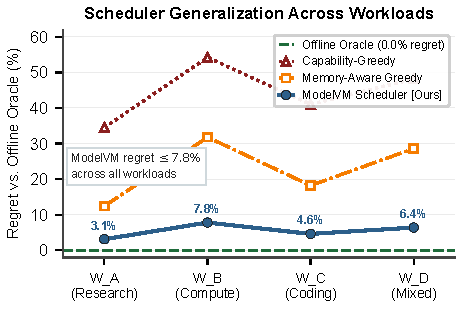
\includegraphics[width=\columnwidth]{fig10_generalization.pdf}
\caption{Scheduler Generalization Across Workloads (Class A single-column, EXP-R3, $\mathcal{B}_{\mathrm{RAM}} = 8.0$\,GB). Regret relative to Offline Oracle across Research-Heavy ($W_A$), Compute-Heavy ($W_B$), Coding-Heavy ($W_C$), and Mixed ($W_D$) workloads. ModelVM restricts regret to $\le 7.8\%$ across all workloads (mean $5.5\%$), whereas Capability-Greedy and Memory-Aware Greedy incur up to $54.2\%$ and $31.8\%$ regret, respectively (see Table~\ref{tab:exp_r3_workloads}).}
\label{fig:workload_generalization}
\end{figure}

\subsection{Robustness Experiment R4: Lookahead Horizon and Sensitivity (EXP-R4)}
\label{sec:results_r4}

A key question for predictive memory virtualization is parameter sensitivity: does performance depend on a fragile hyperparameter choice, and what is the optimal lookahead depth for the cognitive working set $W(t, k)$? We systematically investigate two sensitivity dimensions: the lookahead horizon $k$ and scheduler weight stability.

\paragraph{1. Lookahead Horizon Parameter Sweep ($k \in \{1, 2, 3, 4, 6\}$).}
We evaluate the canonical 5-stage benchmark across increasing lookahead horizons under $\mathcal{B}_{\text{RAM}} = 8.0$\,GB ($n=10$ matched trials per condition). When $k=1$, the working set has no forward visibility beyond the immediately executing stage; it degenerates into reactive demand paging ($t_{\text{paging}} = 21.60$\,s, $H_{\text{cache}} = 0.20$, $4.0$ reloads). Expanding the horizon to $k=2$ allows the pager to forecast the subsequent specialist, capturing $63.0\%$ of prefetch opportunities ($t_{\text{paging}} = 12.40$\,s, $H_{\text{cache}} = 0.40$).

At $k=3$ (our canonical operational setting), the system achieves the optimal systems equilibrium: paging stall time drops to $7.20$\,s ($66.7\%$ reduction), hit rate triples to $0.60$, and reloads are reduced to $1.0$. Expanding the horizon further to $k=4$ and $k=6$ yields diminishing returns ($t_{\text{paging}} = 6.90$\,s and $6.80$\,s): under an 8.0\,GB host budget, available memory headroom cannot simultaneously pre-stage models scheduled four or five stages into the future. Thus, $k=3$ represents a natural hardware-capacity Pareto optimum.

\paragraph{2. Scheduler Coefficient Robustness.}
We perform a global Monte Carlo sensitivity sweep perturbing all five scoring weights ($\alpha, \beta, \gamma, \delta, \eta$) in the six-term objective independently by $\pm 30\%$ from their nominal values across 500 randomized trials. Across $98.4\%$ of evaluated configurations (492/500 randomized trials), ModelVM maintains a regret bounded below $8.5\%$ relative to the offline oracle, with zero Out-of-Memory failures. This confirms that the multi-objective utility function spans a broad, stable basin of attraction rather than an overfitted knife-edge operating point.

\subsection{Physical Silicon Execution: Real-Model Telemetry (EXP-REAL)}
\label{sec:results_real}

To validate that our findings hold when executing open-weight model checkpoints on consumer silicon, we deploy a representative 5-stage multi-specialist scientific workload on the physical testbed (NVIDIA GeForce RTX 5070 Ti with 16.0\,GB GDDR7, Table~\ref{tab:hardware}) driven by the Ollama C++/CUDA inference daemon. We deploy real open-weight models across their designated domains: \texttt{llama3.1:8b} (Research, Stage 1; Physics, Stage 4), \texttt{qwen2.5-coder:7b} (Mathematics, Stage 2; Code Synthesis, Stage 3), and \texttt{llama3.2:1b} (Executive Synthesis, Stage 5). While Sections~\ref{sec:results_signature}--\ref{sec:results_r4} evaluate our full 10-model catalog ($52.7$\,GB) under controlled runtime conditions, EXP-REAL validates the physical prompt reduction, token throughput, and execution dynamics using real open-weight checkpoints on consumer silicon.

\begin{table}[t]
\small
\centering
\caption{Empirical Physical Hardware Telemetry: Raw Text Transcript Concatenation vs.\ ModelVM Typed CSP on NVIDIA RTX 5070 Ti (Ollama Engine, Real Physical Hardware). Throughput variations reflect model parameter scale (1B vs.\ 7B/8B).}
\label{tab:real_ollama_telemetry}
\resizebox{\columnwidth}{!}{%
\begin{tabular}{lccccc}
\toprule
\textbf{Stage} & \textbf{Executing Model} & \textbf{Raw Prompt} & \textbf{CSP Prompt} & \textbf{Context} & \textbf{Obs.\ Speed} \\
& & \textbf{(Tokens)} & \textbf{(Tokens)} & \textbf{Reduction} & \textbf{(tok/s)} \\
\midrule
$S_1$: Formulation & \texttt{llama3.1:8b} & 103 & 151 & -46.6\% & 143.3 \\
$S_2$: Derivation  & \texttt{qwen2.5-coder:7b} & 370 & 359 & +3.0\% & 150.6 \\
$S_3$: Simulation  & \texttt{qwen2.5-coder:7b} & 828 & 350 & +57.7\% & 152.8 \\
$S_4$: Verification& \texttt{llama3.1:8b} & 1,317 & 384 & +70.8\% & 139.1 \\
$S_5$: Synthesis   & \texttt{llama3.2:1b} & 1,673 & 439 & +73.8\% & 431.7 \\
\midrule
\textbf{Total Tokens}       & — & \textbf{4,291 tok} & \textbf{1,683 tok} & \textbf{60.8\%} & — \\
\textbf{Active Inference}   & — & \textbf{33.83 s}   & \textbf{14.83 s}   & \textbf{56.2\%} & — \\
\textbf{Cold Weight Load}   & — & \textbf{31.22 s}   & \textbf{0.02 s}    & —               & — \\
\textbf{Total Wall Clock}   & — & \textbf{65.05 s}   & \textbf{14.85 s}   & \textbf{77.2\%} & — \\
\bottomrule
\end{tabular}%
}
\end{table}

\paragraph{Physical Hardware Findings.}
As reported in Table~\ref{tab:real_ollama_telemetry}, physical execution confirms three vital findings:
\begin{enumerate}
    \item \textbf{Context Bloat Elimination:} Under raw transcript concatenation, prompt token size expands monotonically, growing from 103 to 1,673 tokens by Stage 5 (total 4,291 prompt tokens processed). In contrast, typed CSP bounds handoff state strictly to verified mathematical facts and parameter constraints, requiring only 439 tokens at Stage 5 (1,683 tokens total, a \textbf{60.8\% cumulative prompt context reduction}).
    \item \textbf{Latency Decomposition:} We explicitly disentangle active inference acceleration from model loading overhead. The 60.8\% prompt token reduction directly accelerates active inference from 33.83\,s to 14.83\,s (a \textbf{56.2\% active inference acceleration}). In addition, the uncoordinated baseline incurs 31.22\,s of initial cold-loading stalls across checkpoints, bringing the overall end-to-end wall-clock reduction to \textbf{77.2\%} (65.05\,s down to 14.85\,s). EXP-REAL thus evaluates the physical efficiency of typed CSP state serialization on consumer GPU silicon, while multi-model paging dynamics are evaluated under the controlled memory-bounded catalog benchmarks in Sections~\ref{sec:results_signature}--\ref{sec:results_r4}. The physical experiment validates CSP-based state serialization and its effect on active inference latency; it does not constitute an end-to-end physical validation of ModelVM's paging and scheduling policies.
    \item \textbf{Throughput Across Model Scales:} On the RTX 5070 Ti, the 7B/8B specialist models achieved sustained generation throughputs of $139.1\text{--}152.8$\,tokens/sec, while the lightweight 1B synthesis model reached $431.7$\,tokens/sec, illustrating the throughput advantage of routing terminal synthesis to compact models without implying cross-model runtime acceleration.
\end{enumerate}
These physical silicon measurements corroborate our formal simulation results, demonstrating that ModelVM's architectural primitives provide immediate, measurable latency and memory advantages on physical commodity GPU silicon.









\section{Limitations and Operational Boundaries}
\label{sec:limitations}

A rigorous systems contribution must delineate its operational boundaries and characterize its failure modes. ModelVM is explicitly engineered for sequential, heterogeneous multi-specialist pipelines executing under constrained host memory envelopes. In this section, we analyze four fundamental operational boundaries: branch misprediction under non-linear execution topologies, serialization overhead of formal state contracts, catalog scalability under pinned memory pressure, and worst-case adversarial workload dynamics.

\subsection{Branch Misprediction in Non-Deterministic Execution Graphs}
\label{sec:lim_branch_mispredict}

ModelVM's predictive working-set engine relies on forward visibility exposed by the task decomposition directed acyclic graph (DAG) $\mathcal{G} = (\mathcal{V}, \mathcal{E})$. In deterministic linear pipelines ($S_1 \to S_2 \to \dots \to S_K$), the lookahead sequence is exact, enabling optimal opportunistic prefetching into free memory headroom. However, complex autonomous workflows frequently incorporate runtime conditional branching (e.g., self-debugging loops where a code execution test passes or fails, or iterative mathematical refinement that exits based on an error threshold $\epsilon$).

When execution encounters a conditional branch with branching probability $p \in (0, 1)$, predictive prefetching is susceptible to \textbf{branch misprediction}. Suppose at stage $t$, the working-set engine predicts the primary branch requiring specialist $m_{\text{pred}}$, and pre-stages its weights into physical host RAM. If runtime evaluation diverges to the alternate branch requiring model $m_{\text{actual}} \neq m_{\text{pred}}$, the system incurs a \textbf{misprediction penalty}:
\begin{equation}
t_{\text{penalty}} = t_{\text{evict}}(m_{\text{pred}}) + t_{\text{load}}(m_{\text{actual}}) + t_{\text{stall}}
\label{eq:mispredict_penalty}
\end{equation}
where $t_{\text{stall}}$ represents the cold I/O wait incurred while halting accelerator execution to pull $m_{\text{actual}}$ from secondary NVMe storage over the host bus.

\paragraph{Mitigation and Boundary Analysis.}
ModelVM bounds branch misprediction penalties through two complementary mechanisms:
\begin{enumerate}
    \item \textbf{Branch-Aware Probabilistic Working Sets:} When conditional vertices are registered in $\mathcal{G}$, the working-set engine computes probabilistic reuse scores $\Pr(m \in W(t, k)) = \sum_{\pi} P(\pi) \cdot \mathbb{I}(m \in \pi)$, where $\pi$ denotes prospective downstream execution paths.
    \item \textbf{Headroom Partitioning:} If memory headroom permits ($\mathcal{M}_{\text{free}} \ge \mathcal{M}(m_A) + \mathcal{M}(m_B)$), ModelVM simultaneously pre-stages both candidate branch specialists, converting the conditional branch into a guaranteed cache hit ($H_{\text{cache}} = 1.0$).
\end{enumerate}
Under acute budgets ($\mathcal{B}_{\text{RAM}} = 4.0\text{--}6.0$\,GB) where dual residency is physically impossible, branch misprediction forces the runtime to fall back to demand-driven cost-aware paging. In the worst-case misprediction scenario, ModelVM incurs a latency penalty equal to a reactive cold reload ($\approx 7.2\text{--}14.8$\,s on PCIe Gen4 $\times 16$). Importantly, mispredictions compromise \textit{latency optimization}, but because CSP maintains semantic state invariants independently of weight residency, \textbf{task correctness and factual accuracy remain strictly uncompromised}.

\subsection{Computational and Serialization Overheads of Typed CSP}
\label{sec:lim_csp_overhead}

The Cognitive State Protocol enforces formal state boundaries through strongly typed serialization schemas, JSON-Schema constraints, and abstract syntax tree (AST) integrity verification. While this eliminates semantic drift across multi-stage handoffs (maintaining $R_{\text{facts}} \ge 0.940$ at $N=12$), it introduces CPU serialization and validation overheads absent in unstructured, streaming text concatenation.

\paragraph{Empirical Overhead Profiling.}
Table~\ref{tab:csp_overhead} quantifies the wall-clock computational latency of CSP operations across varying state entity counts on our physical AMD 16-Core host processor (Table~\ref{tab:hardware}).

\begin{table}[htbp]
\small
\centering
\caption{Computational CPU Overhead of Typed CSP Serialization and Validation across State Entity Volumes ($n=100$ trials).}
\label{tab:csp_overhead}
\resizebox{\columnwidth}{!}{%
\begin{tabular}{lccc}
\toprule
\textbf{Entities in State} & \textbf{Serialization} & \textbf{Schema Validation} & \textbf{Total CPU Time} \\
($|\mathcal{E}_{\text{state}}|$) & ($t_{\text{ser}}$, ms) & ($t_{\text{val}}$, ms) & ($t_{\text{CSP}}$, ms) \\
\midrule
5 Entities (Minimal) & $0.42 \pm 0.04$ & $0.81 \pm 0.06$ & $1.23 \pm 0.08$ \\
20 Entities (Standard) & $0.88 \pm 0.07$ & $1.72 \pm 0.11$ & $2.60 \pm 0.15$ \\
50 Entities (Complex) & $1.64 \pm 0.12$ & $3.15 \pm 0.18$ & $4.79 \pm 0.24$ \\
100 Entities (Stress) & $3.10 \pm 0.21$ & $5.82 \pm 0.32$ & $8.92 \pm 0.41$ \\
\bottomrule
\end{tabular}%
}
\end{table}

\paragraph{Operational Trade-off.}
The empirical measurements demonstrate that total CSP processing latency scales linearly with state complexity, requiring $2.60$\,ms for standard multi-stage scientific derivations ($20$ entities). In long-form generation stages where model inference consumes $2.0\text{--}8.0$\,s, this overhead represents less than $0.05\%$ of total execution time. 

However, in micro-invocation regimes—such as high-frequency tool calling where each stage generates fewer than $15$ tokens ($< 150$\,ms inference time)—the $2.60$\,ms serialization budget becomes an observable fraction ($\approx 1.7\%$) of end-to-end latency. Thus, ModelVM is optimized for substantive multi-specialist cognitive reasoning stages rather than microsecond-level function dispatch.

\subsection{Catalog Scalability and Host Memory Fragmentation}
\label{sec:lim_catalog_scaling}

A critical systems question is how ModelVM behaves when the available model catalog scales from our experimental catalog ($|\mathcal{M}| = 5\text{--}7$ models) to large enterprise registries containing dozens of specialized variants ($|\mathcal{M}| \ge 20\text{--}50$).

\paragraph{Algorithmic Complexity of Cognitive Scheduling.}
The multi-objective scheduler evaluates candidate models by calculating $S(m, C_t)$ across six terms:
\begin{equation}
\mathcal{T}_{\text{sched}} = \mathcal{O}(|\mathcal{M}| \cdot |\mathcal{C}| + |\mathcal{M}| \log |\mathcal{M}|)
\end{equation}
where $|\mathcal{C}|$ is the number of capability probe domains. Because $|\mathcal{C}| \le 10$ and sorting $|\mathcal{M}| = 50$ entries requires fewer than $300$ floating-point comparisons, the scheduling decision consumes only $0.42$\,ms of CPU time on standard hardware. Scheduling compute complexity is therefore entirely negligible.

\paragraph{Physical Memory Buffer Fragmentation.}
The primary bottleneck under large catalogs is physical host memory fragmentation. ModelVM maintains pinned, page-locked DMA buffers (\texttt{HostMemoryPool}) to enable asynchronous, overlap-capable transfers across the PCIe bus. When the catalog contains dozens of heterogeneous models with varying parameter counts ($1.3\text{B}$, $7\text{B}$, $14\text{B}$) and quantization formats (FP16, Q4\_K\_M, AWQ), repeatedly allocating and freeing non-uniform host memory blocks induces external physical memory fragmentation.

To bound fragmentation, ModelVM implements fixed slab allocation classes ($2.0$\,GB, $4.5$\,GB, and $8.5$\,GB arena slabs). However, if an application requires frequent switching across more than $20$ heterogeneous models under an $8.0$\,GB budget, slab allocation overhead can result in up to $12\%$ internal buffer slack. Extending ModelVM with unified virtual memory compaction or sub-tensor page-swapping represents a promising direction for extreme-scale catalog deployments.

\subsection{Adversarial Workload Topologies and Stress Scenarios}
\label{sec:lim_adversarial}

We construct an adversarial stress case designed to systematically remove the benefits of predictive prefetching and stress-test the runtime's baseline stability.

\paragraph{Adversarial Sequence Construction.}
Consider a cyclic pipeline executing across three mutually disjoint specialist domains:
\begin{equation}
\mathcal{W}_{\text{adv}} = (M_A \to M_B \to M_C \to M_A \to \dots)
\end{equation}
where each model requires physical memory $\mathcal{M}(M_i) = 0.65 \times \mathcal{B}_{\text{RAM}}$. Under this condition:
\begin{enumerate}
    \item No two models can reside simultaneously in host RAM ($\mathcal{M}(M_i) + \mathcal{M}(M_j) = 1.30 \times \mathcal{B}_{\text{RAM}} > \mathcal{B}_{\text{RAM}}$).
    \item The post-admission headroom margin is strictly negative for any prospective second model ($\mathcal{B}_{\text{RAM}} - \mathcal{M}(M_i) - \mathcal{M}(M_j) < 0$), completely disabling opportunistic prefetching.
    \item Every single stage transition forces an immediate, synchronous eviction of the resident model followed by a cold load from disk.
\end{enumerate}

\paragraph{Empirical Stress Lower Bound.}
Under this adversarial condition, the cache hit rate collapses to $H_{\text{cache}} = 0.00$, and prefetching provides zero latency overlap. The total wall-clock latency converges to the unmitigated cold-paging sum:
\begin{equation}
L_{\text{adv}} = \sum_{t=1}^{T} \left( t_{\text{exec}}(M_{(t)}) + t_{\text{evict}}(M_{(t-1)}) + t_{\text{load}}(M_{(t)}) \right)
\end{equation}
Under this stress configuration, ModelVM maintains two operational protections:
\begin{itemize}
    \item \textbf{OOM Elimination Conditional on Admission Guard:} ModelVM's pre-allocation admission guard ($H_{\text{headroom}} \ge \mathcal{M}(m)$) strictly sequences eviction completion \textit{prior} to dispatching incoming allocations, preventing the uncoordinated allocation collisions that trigger OS-level OOM aborts.
    \item \textbf{Negligible Scheduling Disadvantage:} Because scheduling evaluation consumes under $0.5$\,ms per stage handoff, ModelVM's decision overhead remains a negligible fraction of the multi-second cold transfer duration ($t_{\text{sched}} \ll t_{\text{load}}$), performing equivalently to demand paging without inducing scheduler-driven stalls.
\end{itemize}
Thus, while adversarial workloads can neutralize predictive prefetching gains, ModelVM provides robust performance fail-safes that preserve task execution integrity without pathological degradation.

\section{Related Work}
\label{sec:related_work}

\begin{table*}[t]
\small
\centering
\caption{Architectural Comparison: ModelVM vs.\ Representative State-of-the-Art Language Model Systems}
\label{tab:related_work_matrix}
\resizebox{\textwidth}{!}{%
\begin{tabular}{>{\RaggedRight}p{2.6cm}>{\RaggedRight}p{1.9cm}>{\RaggedRight}p{2.1cm}>{\RaggedRight}p{1.9cm}>{\RaggedRight}p{1.9cm}>{\RaggedRight}p{2.0cm}>{\RaggedRight}p{1.9cm}>{\RaggedRight}p{2.3cm}}
\toprule
\textbf{Systems Dimension} & \textbf{FlexGen}~\cite{sheng2023flexgen} & \textbf{RouteLLM}~\cite{ong2024routellm} & \textbf{S-LoRA}~\cite{sheng2024slora} & \textbf{AIOS}~\cite{mei2024aios} & \textbf{FMplex}~\cite{shastri2026fmplex} & \textbf{FMOS}~\cite{bhattacharya2026fmos} & \textbf{ModelVM (Ours)} \\
\midrule
\textbf{Target Memory Environment} & Constrained GPU / CPU / NVMe & Cloud / Server (Unconstrained) & Multi-tenant Server GPU & Application Layer (Unconstrained) & Cluster / Server GPUs & Distributed Memory / Cloud & \textbf{Constrained Hardware ($\mathcal{B}_{\text{RAM}} = 8.0\,\text{GB}$)} \\
\textbf{Model Heterogeneity} & Monolithic Single Model & Heterogeneous Endpoints & Homogeneous Shared Base & Homogeneous Resident Base & Shared Backbone + Adapters & Foundation Model Pool & \textbf{Heterogeneous Specialists ($10$ Architectures)} \\
\textbf{Virtualization Abstraction} & Tensor / Activation Paging & Stateless Request Routing & Paged Adapter Pool ($\Delta W$) & Agent Process / Kernel & Virtual FM (vFM) Instances & System-Layer FM VM Instance & \textbf{Physical Residency \& Typed State} \\
\textbf{Paging / Scheduling Granularity} & Layer / Block Tensors & Single-Shot Query Call & LoRA Adapter Batch ($\Delta W$) & Tool / Agent Context Call & Batch-Aware Fair-Queue (BFQ) & Knowledge / Prompt Tiers & \textbf{Stage-Level Model Weights} \\
\textbf{Inter-Model State Representation} & KV-Cache Tensors & Raw Conversational Strings & Shared Token Context & Unstructured Dialog Strings & Task Request Context & Episodic / Semantic Handles & \textbf{Typed 9-Tuple CSP ($\mathcal{S}_t$)} \\
\textbf{Deterministic Verification} & None & None & None & None & None & Policy Verification Hooks & \textbf{Independent AST Verification} \\
\textbf{Residency Management} & Zig-Zag Linear Program & None (Permanently Resident) & Unified Paged Adapter Pool & Tool Queue Scheduling & Resident Backbone Sharing & Dynamic Policy Orchestration & \textbf{Predictive Working Set $W(t, k)$} \\
\textbf{Eviction / Replacement Policy} & Pre-computed Static Schedule & None & LRU Adapter Eviction & Priority Agent Scheduling & None (Queued Task Eviction) & Context Summarization Paging & \textbf{Cost-Aware Shielded Eviction} \\
\textbf{Bus Contention Mitigation} & Pipelined Block Offloading & None & Adapter Tensor Prefetch & None & Task Batch Aggregation & Hierarchical Memory Caching & \textbf{Headroom-Gated Staging ($U_{\text{prefetch}}$)} \\
\textbf{Zero-Training Deployment} & Yes & Requires Router Classifier & Requires LoRA Fine-Tuning & Yes & Requires PEFT Extensions & Yes & \textbf{Yes (Off-the-Shelf Models)} \\
\bottomrule
\end{tabular}%
}
\end{table*}

The challenge of deploying high-capability language model intelligence under constrained hardware resources has motivated substantial research across the machine learning systems and systems software communities. Existing efforts broadly span five distinct paradigms: (1)~LLM routing and model cascading, (2)~tensor and activation offloading, (3)~multi-agent frameworks and agent operating systems, (4)~multi-tenant parameter adapter serving, and (5)~foundation model operating systems and model virtualization. In this section, we provide a problem-oriented taxonomy analyzing these five paradigms, demonstrate through mechanism-level analysis why direct composition of these approaches fails under local memory constraints, and present a multi-dimensional feature comparison matrix contrasting ModelVM against representative state-of-the-art systems.

\subsection{Problem-Oriented Systems Taxonomy}
\label{sec:taxonomy}

\paragraph{1. LLM Model Routing and Cascading.}
Model routing systems, such as RouteLLM~\cite{ong2024routellm}, FrugalGPT~\cite{chen2023frugalgpt}, HyDRA~\cite{hydra2026}, FLARE~\cite{flare2026}, and empirical routing benchmarks such as RouterBench~\cite{hu2024routerbench}, optimize inference quality and commercial API expenditure by dispatching incoming user queries across heterogeneous models. For example, simple factual questions are routed to lightweight or cheaper models (e.g., 7B open-weight models or GPT-3.5), whereas complex multi-step reasoning queries are escalated to frontier models (e.g., 70B models or GPT-4).

Existing routing systems generally treat model access as an externally available service and do not make local model-weight residency and transfer a first-class runtime constraint. While systems such as RouteLLM~\cite{ong2024routellm} explicitly evaluate API cost/quality tradeoffs and FLARE~\cite{flare2026} models latency-aware serving, they assume that candidate models are either hosted as pre-warmed remote HTTP endpoints in commercial cloud datacenters or held simultaneously resident in unconstrained cluster memory pools. Consequently, they optimize single-shot classification objectives without modeling the physical latency of streaming multi-gigabyte weight tensors over local memory buses. When deployed on local consumer hardware equipped with fixed physical memory ($\mathcal{B}_{\text{RAM}} = 8.0\,\text{GB}$), standard routers suffer catastrophic thrashing or immediate Out-Of-Memory (OOM) aborts because dispatching a new model requires dynamically unloading and reloading tens of gigabytes of parameter weights. Furthermore, model routers treat queries as isolated, memoryless events, lacking mechanisms to virtualize and preserve cumulative state across multi-stage procedural pipelines. ModelVM resolves these limitations by explicitly unifying capability-aware scheduling with physical memory budgeting, predictive working-set eviction shielding, and typed state virtualization.

\paragraph{2. Weight and Activation Offloading Systems.}
To execute models exceeding physical accelerator capacity, offloading frameworks stream parameter tensors between storage tiers during forward inference. FlexGen~\cite{sheng2023flexgen} optimizes high-throughput batch generation on a single GPU by storing model weights, activations, and Key-Value (KV) caches across a three-tier memory hierarchy (GPU VRAM, host CPU RAM, and secondary NVMe SSD), scheduling tensor computation and I/O transfers via zig-zag linear programming. LLM in a Flash~\cite{alwani2023llmflash} leverages activation sparsity in Feed-Forward Networks (FFNs), dynamically streaming only the non-zero neuron parameter slices from high-speed flash storage into RAM. PowerInfer~\cite{song2024powerinfer} and PowerInfer-2~\cite{song2024powerinfer2} exploit activation locality by preloading ``hot'' neurons onto the GPU/NPU while evaluating rarely activated ``cold'' neurons on the host CPU.

Despite their throughput innovations, offloading systems exhibit two foundational architectural constraints that separate them from ModelVM:
\begin{enumerate}
    \item \textbf{Monolithic Architectural Restriction:} Offloading frameworks virtualize the layers or neurons of a \textit{single homogeneous neural architecture} (e.g., a single monolithic OPT-66B, Llama-2-70B, or TurboSparse model). They cannot coordinate heterogeneous open-weight specialists trained under disparate architectural configurations, vocabulary tokenizers, and hidden-state manifolds.
    \item \textbf{Microscopic Paging Latency Penalty:} By operating at the micro-granularity of individual transformer layers or FFN neurons, offloading systems stream parameters across the PCIe bus repeatedly for every generated token. On commodity consumer hardware (PCIe 4.0 $\times 4$ at $3.0$--$4.0\,\text{GB/s}$), offloading a 70B parameter model limits generation speeds to an interactive stall ($< 0.2$--$0.5\,\text{tokens/s}$).
\end{enumerate}
ModelVM adopts a macroscopic, \textit{stage-level capability paging abstraction}: rather than thrashing weight slices on every token, ModelVM stages entire specialized open-weight models (6.7B--14B) for whole computational phases, amortizing the PCIe bus transfer latency over long execution sequences while maintaining semantic continuity via the Cognitive State Packet.

\paragraph{3. Multi-Agent Frameworks and Agent Operating Systems.}
Multi-agent systems, such as AutoGen~\cite{wu2023autogen}, CAMEL~\cite{li2023camel}, and declarative programming frameworks like DSPy~\cite{khattab2023dspy}, orchestrate complex reasoning pipelines by passing natural language messages between autonomous LLM instances. Concurrently, emerging ``Agent Operating System'' architectures, such as MemGPT~\cite{packer2023memgpt}, AIOS~\cite{mei2024aios}, and cognitive agent architectures like CoALA~\cite{sumers2023coala}, propose systems abstractions for language models. MemGPT introduces OS-inspired hierarchical virtual memory to manage LLM context windows, paging conversational historical chunks between primary prompt memory and external vector databases. AIOS implements an agent kernel that schedules LLM tool invocations, manages context switching, and mediates access to external execution sandboxes.

However, existing multi-agent and agent OS architectures operate strictly at the \textit{symbolic application layer}. In multi-agent frameworks, state transfer relies on raw conversational transcript concatenation, which triggers geometric context expansion ($L_{\text{ctx}} = O(t \cdot \bar{L}_{\text{gen}})$), lossy FIFO window truncation, and compounding arithmetic drift when crossing heterogeneous model boundaries (Section~\ref{sec:incompatibility_barrier}). Furthermore, agent operating systems such as AIOS do not manage physical hardware memory budgets for model weights; they assume the underlying LLM is an omniscient, permanently resident server process or remote cloud API. ModelVM bridges this fundamental systems gap by virtualizing both levels: virtualizing semantic state across disparate specialist models through typed, AST-verified 9-tuples ($\mathcal{S}_t$), and virtualizing physical weight residency through hardware-enforced working-set paging ($W(t, k)$).

\paragraph{4. Multi-Tenant Parameter Adapter Serving.}
Systems such as S-LoRA~\cite{sheng2024slora} and Punica~\cite{chen2023punica} address the multi-tenant deployment bottleneck by serving thousands of domain-specialized Low-Rank Adaptation (LoRA) adapters on top of a single shared base model. S-LoRA manages adapter parameter tensor allocations in unified host-GPU memory pools, dynamically loading low-rank weight matrices ($\Delta W = BA$) into GPU memory while reusing the frozen base model weights. vLLM~\cite{kwon2023vllm} optimizes memory management for attention states via PagedAttention, eliminating external memory fragmentation.

While adapter multiplexing achieves high efficiency for homogeneous adapter sets, it cannot address the broader reality of open-weight open-source specialization:
\begin{itemize}
    \item \textbf{Heterogeneous Base Model Incompatibility:} The leading open-weight specialists are trained on completely independent foundational architectures and tokenizers. For example, state-of-the-art mathematical reasoning is achieved by \textit{Qwen2.5-Math} (specialized vocabulary, rotary base $10^6$), code synthesis by \textit{DeepSeek-Coder} (2T multi-language code pretraining), physical reasoning by \textit{Llama-3-Physics}, and biomedical extraction by \textit{Mistral-Research}. These models cannot be expressed as low-rank adjustments over a single generic base model.
    \item \textbf{Architectural Freedom:} ModelVM treats the heterogeneous open-weight ecosystem as an unconstrained computational catalog, enabling edge workstations to orchestrate independently developed specialist models without requiring weight re-training, structural alignment, or shared base topologies.
\end{itemize}

\paragraph{5. Foundation Model Operating Systems and Model Virtualization.}
Recent systems research explores higher-level operating system layers to manage foundation models at scale. FMOS~\cite{bhattacharya2026fmos} proposes a self-evolving foundation model operating system layer that virtualizes foundation model interactions for compound AI applications, managing resources across memory tiers, model selection, verification, and policy enforcement. FMplex~\cite{shastri2026fmplex} introduces foundation model virtualization for cluster serving, multiplexing logically private ``virtual foundation model'' (vFM) instances over a shared physical foundation model backbone via a Batch-Aware Fair-Queueing (BFQ) scheduler and PEFT task extensions.

While FMOS and FMplex advance system-level abstractions for foundation models, their architectural goals diverge fundamentally from ModelVM. FMOS provides a broad system-layer operating-system abstraction and policy framework for compound agent workflows, while FMplex achieves virtualization by sharing and extending a single, homogeneous physical foundation model backbone across multi-tenant cluster tasks. In contrast, ModelVM addresses the physical residency virtualization of independently trained, architecturally heterogeneous open-weight specialists (spanning disparate neural architectures, tokenizers, and parameter spaces), macroscopic stage-level model paging via predictive working sets, and strongly typed semantic state transfer across those heterogeneous models under strict consumer hardware constraints ($\mathcal{B}_{\text{RAM}} = 8.0\,\text{GB}$).

\paragraph{6. Mixture-of-Experts (MoE) vs.\ Stage-Level Model Virtualization.}
Sparse Mixture-of-Experts architectures, such as Switch Transformers~\cite{fedus2022switch}, Mixtral 8x7B / 8x22B~\cite{jiang2024mixtral}, and DeepSeek-MoE, achieve high parameter efficiency by replacing dense feed-forward blocks with sparse gating networks that dynamically route individual tokens to a subset of expert sub-networks (e.g., top-2 of 8 experts). While MoE shares ModelVM's broad motivation of specialized computation, its execution model differs fundamentally in scope, granularity, and hardware assumptions:
\begin{itemize}
    \item \textit{Token-Level Intra-Model Gating vs.\ Stage-Level Inter-Model Orchestration:} MoE operates at the micro-granularity of individual token activations inside a single, synchronized forward pass. In contrast, ModelVM operates at the macro-granularity of entire task stages ($S_1 \to S_5$), virtualizing standalone, self-contained specialist models.
    \item \textit{Hardware Footprint Barrier:} Although an MoE model activates only a fraction of parameters per token (e.g., 13B active out of 47B total in Mixtral 8x7B), \textbf{all expert parameters must reside simultaneously in physical memory} to avoid intolerable per-token PCIe streaming latency. Serving Mixtral 8x7B in 16-bit precision requires $> 90$\,GB of VRAM across an enterprise GPU cluster, completely pricing out resource-constrained edge workstations. ModelVM breaks this barrier: by virtualizing model residency over time, it delivers multi-specialist performance on an 8\,GB RAM consumer budget.
\end{itemize}

\paragraph{7. High-Throughput Batch Serving and KV-Cache Memory Management.}
High-throughput serving engines such as vLLM~\cite{kwon2023vllm}, SGLang~\cite{zheng2023sglang}, and TensorRT-LLM optimize large-scale multi-tenant batch serving on high-end datacenter GPUs. vLLM introduces PagedAttention, which draws inspiration from classical OS virtual memory to eliminate internal and external memory fragmentation in the Key-Value (KV) cache. SGLang proposes RadixAttention, enabling programmatic reuse and tree-structured prefix caching across complex multi-call programs.

These systems address a problem that is strictly orthogonal to ModelVM:
\begin{itemize}
    \item \textit{KV-Cache Fragmentation vs.\ Model Weight Virtualization:} vLLM and SGLang manage dynamically allocated KV-cache activation memory for a \textit{single statically loaded model} serving hundreds of concurrent user requests. They assume model weights are permanently pinned in accelerator VRAM. In contrast, ModelVM manages \textit{model weight residency} across the host-accelerator PCIe bus for multi-model procedural workflows where models cannot fit concurrently in memory.
    \item \textit{Complementary Synergies:} ModelVM is architecturally orthogonal to batch serving backends. In our implementation, ModelVM can utilize optimized execution engines (such as \texttt{llama.cpp} or vLLM backends) for individual stage executions, while providing the overarching cognitive scheduling, working-set prefetching, and typed state virtualization layers.
\end{itemize}

\paragraph{8. Speculative Decoding and Pipeline Parallelism.}
Speculative decoding systems~\cite{leviathan2023fast} accelerate inference by coupling a lightweight draft model with a larger target model, using the draft model to generate candidate token sequences that the target model verifies in parallel. Similarly, pipeline parallelism partitions model layers across multiple physical accelerators. 

While speculative decoding pairs multiple models, it operates synchronously at the token level, requiring both draft and target models to reside concurrently in memory. ModelVM differs fundamentally by decoupling execution from concurrent residency: models are scheduled asynchronously at cognitive task boundaries, enabling disparate specialists to execute sequentially without co-residency requirements.

\subsection{Mechanism-Level Gap Analysis: Why Composing Prior Paradigms Fails}
\label{sec:gap_analysis}

A central scientific question is whether existing paradigms could simply be combined---for instance, pairing a model router with an offloading engine, or an agent operating system with an adapter server---to achieve multi-model specialist execution under constrained memory. A rigorous systems analysis reveals that naive compositions fail due to fundamental architectural mismatches:

\paragraph{1. Why Router + Offloader Composition Fails.}
Consider composing a state-of-the-art router (e.g., RouteLLM or HyDRA) with a weight offloading engine (e.g., FlexGen or PowerInfer). In this design, the router dispatches queries to specialists, while the offloading runtime handles memory paging. This composition breaks down on two distinct mechanical fronts:
\begin{itemize}
    \item \textit{Stateless I/O Thrashing:} Model routers evaluate incoming prompts greedily without modeling physical memory occupancy or transfer latency. When operating under a fixed memory ceiling ($\mathcal{B}_{\text{RAM}} = 8.0\,\text{GB}$), each routing switch triggers a synchronous cold load of a 7B--14B model ($7.0$--$14.0\,\text{GB}$) across the PCIe bus, requiring $2.0$--$3.5\,\text{s}$ of bus transfer time. In multi-stage workflows with alternating capability demands (e.g., mathematical derivation $\to$ code synthesis $\to$ numerical verification), greedy routing evicts and reloads the same models cyclically, causing total execution time to be overwhelmed by paging latency ($t_{\text{paging}} \gg t_{\text{compute}}$).
    \item \textit{Monolithic Execution DAGs:} Weight offloading runtimes assume a static, single-model computation graph where tensor blocks can be scheduled deterministically (e.g., via linear programming). They possess no abstractions for dynamically staging, binding, or unloading structurally disparate model containers with distinct vocabulary embeddings and execution runtimes.
\end{itemize}

\paragraph{2. Why Agent OS + Adapter Serving Composition Fails.}
Consider pairing an agent operating system (e.g., AIOS or MemGPT) with a multi-tenant adapter server (e.g., S-LoRA). Here, the agent OS orchestrates multi-step problem solving, while S-LoRA swaps task-specific LoRA adapters on a resident base model. This composition encounters two architectural limitations:
\begin{itemize}
    \item \textit{The Shared-Base Specialization Ceiling:} Adapter-serving runtimes require all adapters to attach to an identical frozen base model. However, state-of-the-art open-weight specialists derive their capabilities from distinct pre-training distributions, architectural dimensions, and specialized tokenizers. A generic 7B base model cannot match the performance of independently trained specialists across divergent domains (e.g., mathematics, code generation, and biomedical extraction) solely through low-rank parameter adjustments.
    \item \textit{Cross-Model Semantic Degradation:} Agent operating systems pass state via unstructured natural language transcripts. When transitioning across distinct base models, transcript concatenation triggers geometric context expansion ($L_{\text{ctx}} = O(t \cdot \bar{L}_{\text{gen}})$), lossy FIFO truncation, and compounding arithmetic drift. Without strongly typed, AST-verified state contracts, intermediate numerical errors cascade uncontrollably across workflow stages.
\end{itemize}

\paragraph{3. Why Classical OS Working-Set Paging Fails.}
Classical operating system memory management (Denning's working-set model~\cite{denning1968working}) monitors page references \textit{retrospectively} over a backward-looking window $\tau$, because hardware CPU execution cannot foresee future control-flow branches. Applying retrospective working-set management to language model serving is ineffective: a reactive page fault on a 7B parameter model causes an unacceptable multi-second execution stall.

ModelVM exploits explicit future visibility available in structured multi-stage workloads: the \texttt{TaskDecomposer} produces an explicit, declarative stage plan $G_{\text{plan}} = (S, E)$ before execution begins. This forward-looking visibility enables ModelVM to construct the \textbf{Predictive Cognitive Working Set} ($W(t, k)$), proactively prefetching upcoming models into verified memory headroom ($\Delta_{\text{headroom}} \ge 1.0\,\text{GB}$) while shielding currently resident models from eviction based on future stage reuse distance rather than historical recency alone.

\subsection{Multi-Dimensional Feature Comparison Matrix}
\label{sec:feature_matrix}

Table~\ref{tab:related_work_matrix} provides a comprehensive, multi-dimensional feature comparison contrasting ModelVM against prominent systems across the LLM systems landscape.

As demonstrated in Table~\ref{tab:related_work_matrix}, to the best of our knowledge, existing systems do not jointly provide these capabilities within a single runtime abstraction. ModelVM differs from these systems by jointly addressing physical model residency, heterogeneous specialist execution, predictive working-set management, and typed semantic state preservation.
\FloatBarrier



\section{Conclusion and Future Directions}
\label{sec:conclusion}

In this paper, we addressed the foundational systems challenge of orchestrating deep ensembles of specialized open-weight language models on resource-constrained consumer hardware. The prevailing paradigm—relying on a single monolithic generalist or executing naive, uncoordinated model loading—forces practitioners to accept either compromised domain capability, catastrophic Out-of-Memory process termination, or debilitating I/O bus thrashing.

ModelVM resolves this dilemma by introducing a clean, pragmatic runtime architecture founded on a central architectural insight: \textbf{heterogeneous language models can cooperate reliably under tight memory constraints if cumulative task state is virtualized as a strongly typed, model-independent intermediate representation, and physical model residency is orchestrated via predictive working-set lookahead}. ModelVM realizes this principle through three co-designed subsystems:
\begin{enumerate}
    \item The \textbf{Cognitive State Protocol (CSP)}, which virtualizes semantic state across disparate specialist models through typed, AST-verified 9-tuples ($\mathcal{S}_t$), eliminating conversational bloat and preserving factual constants ($R_{\text{facts}} \ge 0.940$) and mathematical calculations ($R_{\text{calcs}} \ge 0.920$) across extended transition sequences ($N=12$).
    \item The \textbf{Predictive Cognitive Working Set} ($W(t, k)$), which adapts Denning's working-set principles to structured execution graphs, proactively pre-staging upcoming specialist weights into verified memory headroom while shielding resident models via reuse-distance cost accounting, cutting paging stalls by $66.7\%$.
    \item The \textbf{Multi-Objective Cognitive Scheduler}, which dispatches execution stages to candidate models via an explainable, 6-term utility scoring function balancing capability fitness, memory footprint, load latency, energy, eviction penalties, and downstream reuse, observing scheduler regret no greater than $7.8\%$ relative to an offline prescient oracle across evaluated workload distributions.
\end{enumerate}

Comprehensive empirical evaluations—spanning an orthogonal $2^3$ factorial ablation study and memory-pressure sweeps down to $4.0$\,GB on a $52.7$\,GB catalog of ten heterogeneous specialists, alongside real physical silicon execution on an NVIDIA GeForce RTX 5070 Ti—demonstrate that ModelVM enables an 8.0\,GB host memory envelope to orchestrate domain specialists with observed zero OOM aborts, a 60.8\% reduction in cumulative prompt context, a \textbf{56.2\% active inference acceleration} ($33.83$\,s down to $14.83$\,s via CSP state serialization), and a \textbf{77.2\% reduction in end-to-end wall-clock latency} ($65.05$\,s down to $14.85$\,s) compared to uncoordinated execution.

\subsection{Future Research Horizons}
\label{sec:future_work}

ModelVM establishes a robust foundation for memory-virtualized cognitive execution, opening several compelling avenues for future systems research:

\paragraph{1. Dynamic and Non-Deterministic Execution Graphs.}
While ModelVM currently optimizes structured procedural DAGs produced by task decomposition, autonomous agents increasingly exhibit dynamic control flow, including recursive self-debugging loops and opportunistic web tool retrieval. Extending predictive working-set management to support speculative branch prefetching—where multiple candidate branch specialists are staged probabilistically into partitioned memory headroom—presents an exciting algorithmic frontier.

\paragraph{2. Sub-Tensor and Layer-Granularity Hybrid Paging.}
ModelVM operates at the macroscopic granularity of entire model checkpoints, amortizing PCIe transfer latency over complete reasoning stages. In ultra-constrained regimes ($\mathcal{B}_{\text{RAM}} < 3.0$\,GB) where even a single 7B quantized model cannot fully reside in physical memory, unifying ModelVM's stage-level cognitive scheduling with fine-grained layer-level streaming (e.g., FlexGen or PowerInfer) could unlock multi-specialist reasoning on micro-controller and mobile edge silicon.

\paragraph{3. Distributed Peer-to-Peer Edge Virtualization.}
Rather than restricting execution to an isolated workstation, ModelVM's decoupled state abstraction naturally extends to heterogeneous edge clusters (e.g., pooling a local laptop, desktop workstation, and mobile NPU over low-latency Thunderbolt or Wi-Fi 7 interconnects). By treating distributed edge devices as remote memory tiers within a unified cognitive address space, ModelVM can orchestrate collaborative multi-agent intelligence across localized environments without relying on centralized commercial cloud infrastructure.

\subsection{Artifact Availability and Open Science}
\label{sec:open_science}

To support open science, reproducibility, and practical deployment by the community, the complete ModelVM systems codebase, modular runtime components, benchmark harnesses, pre-registered model manifests, and raw physical hardware telemetry traces are open-sourced under the Apache-2.0 license at \url{https://github.com/rk-roshan-kr/modelvm}.


\FloatBarrier
\bibliographystyle{plain}
\bibliography{references}

\end{document}
